% !TeX spellcheck = es_ES
%\chapter{Cap\'{\i}tulo 3}
%\chapter{Solution Proposal}
\chapter{Propuesta de solución}\label{cap:Solucion}
En este Capítulo se propone un modelo ejecutable para la simulación multifísica de procesos de recobro mejorado en yacimientos de petróleo basado en esquemas preconceptuales. Con este fin, se presenta un uso adicional del elemento ``función'' definido en los EP. Además, se plantea usar operadores sobre arreglos para facilitar el desarrollo de la representación del dominio de la simulación de procesos EOR. Luego, se conceptualizan los términos derivados de las ecuaciones que se presentan en el marco teórico. Posteriormente, se muestra el EP completo de la simulación y se explica por secciones los eventos que procesan la simulación.

%Este Capítulo se estructura así: en la Sección \ref{sec:PSNew} se presentan las subrutinas definidas por el usuario como una extensión para las funciones de los EP que permite reutilizar una representación en múltiples secciones del EP y la regla para la obtención de código a partir del nuevo elemento. En la sección \ref{sec:Concepts} se revisan los términos de cada ecuación y su traducción a los conceptos presentes en el EP junto con sus respectivas relaciones estructurales y dinámicas. En la sección \ref{sec:PS_EOR} se muestra el EP completo y se explican los eventos que procesan la simulación.

%%%%%%%%%%%%%%%%%%%%%%%%%%%%%%%%%%%%%%%%%%%%%%%%%%%%%%%%%%%%%%%%
%(Acá debo hablar del proceso tal como lo voy guiando en el esquema preconceptual, es decir, la cadena de implicaciones explicando el paso a paso. Debo reorganizar la información y darle la importancia que se merece a los elementos que estoy GENERALIZANDO!)
%%%%%%%%%%%%%%%%%%%%%%%%%%%%%%%%%%%%%%%%%%%%%%%%%%%%%%%%%%%%%%%%%
%In this section we propose one element as an extension for Preconceptual Schemas(PS) which aid the understanding of diverse elements in the oil reservoir simulation domain. In addition, we present further description of the concepts stated in the theoretical framework, with their respective representation in the elaborated PS.
%This section is structured as follows: in section  we present the added elements to PS and their usage in our represented domain. In section  we propose the representation of structural and dynamical behavior of each developed concept in the theoretical framework using PS.

%\section{Added elements to Preconceptual Schemas}\label{sec:PSNew}
%\subsection{Analyst defined subroutines}\label{sec:PS_ADS}
%Analyst defined subroutines are analyst defined functions as proposed by (ref Calle) without the return argument. They use global elements and parameters of the subroutine definition. They are defined for re-using dynamical behavior elements which appear more than once in the PS. Names of both subroutines and functions must differ from operators predefined in the PS. Graphic symbol used for subroutines is the same as used for operators and functions. In figure \# we present graphical representation of analyst defined subroutines.

%\section{Extensión a las Funciones del Esquema Preconceptual}\label{sec:PSNew}
\section{Subrutinas que define el analista}\label{sec:PS_ADS}
Las subrutinas que define el analista son funciones tal como \cite{JCalle} propone, pero carecen de un concepto de retorno. Estas utilizan elementos globales y también pueden recibir parámetros adicionales; su representación gráfica es igual a la de una función, pero éstas carecen de asignación cuando se usan como operadores. En la Figura \ref{fig:Subroutine} se ilustra un ejemplo de subrutina que se usa en el desarrollo de esta Tesis. %\citep{AG01}.
%Nota: Poner tabla y gráfica de uso

\begin{figure}[h]
	\centering%
	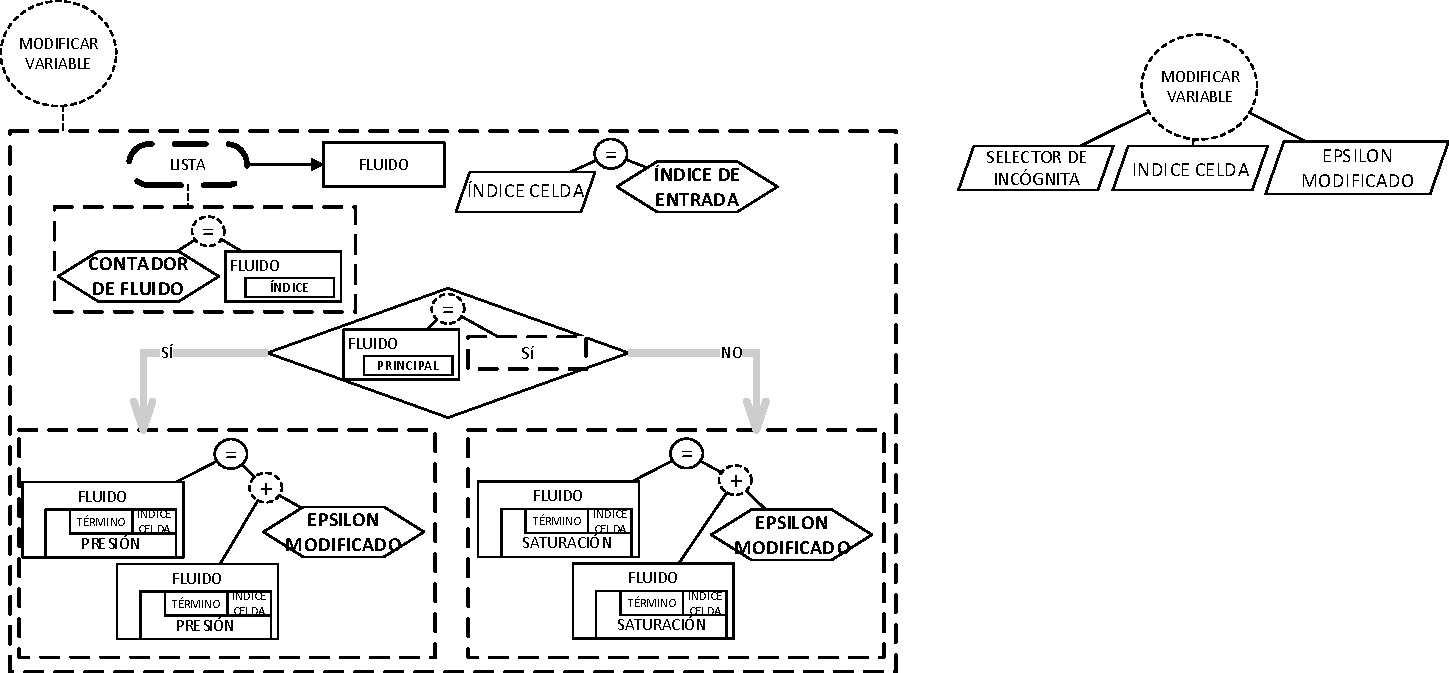
\includegraphics[width=\linewidth]{Fig/SubrutinaEjemplo.pdf}%
	\caption[Subrutina Modificar Variable.]{Subrutina Modificar Variable. Los autores.} \label{fig:Subroutine}
\end{figure}

En la parte izquierda de la Figura \ref{fig:Subroutine} se ve  la definición de la subrutina ``Modificar Variable'', mientras que en la derecha se ve su uso en el EP, que posteriormente aparece en el evento ``Presión del fluido varía''. Es posible notar que la subrutina recibe tres parámetros de entrada, el ``contador del fluido'', el ``índice de entrada'' y el ``épsilon modificado''. Además, en esta se accede a atributos del concepto fluido; y no tiene concepto de retorno.

\section{Operadores sobre arreglos}\label{sec:PS_Operators}
Los operadores sobre arreglos son aquellos que pueden tomar un arreglo por parámetro y evaluar expresiones matemáticas con los elementos del mismo. Para indicar que se está accediendo a todos los elementos del arreglo, se usa un ``\textbf{*}'' en el índice del mismo, tal como se muestra en la Figura \ref{fig:Access}.\\

\begin{figure}[h]
	\centering%
	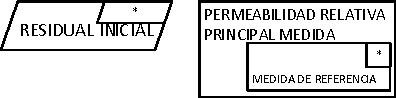
\includegraphics[scale=1]{Fig/EjemploAcceso.pdf}%
	\caption[Índice de acceso ``*'' en arreglos.]{Índice de acceso ``*'' en arreglos. Los autores.} \label{fig:Access}
\end{figure}

En la Figura \ref{fig:Operators} se muestran tres ejemplos de uso, uno en conceptos tipo arreglo, y otros dos de arreglos independientes. Se destaca que las operaciones no se definen en el EP. En la programación, éstas se usan desde alguna librería o función del lenguaje.

\begin{figure}[h]
	\centering%
	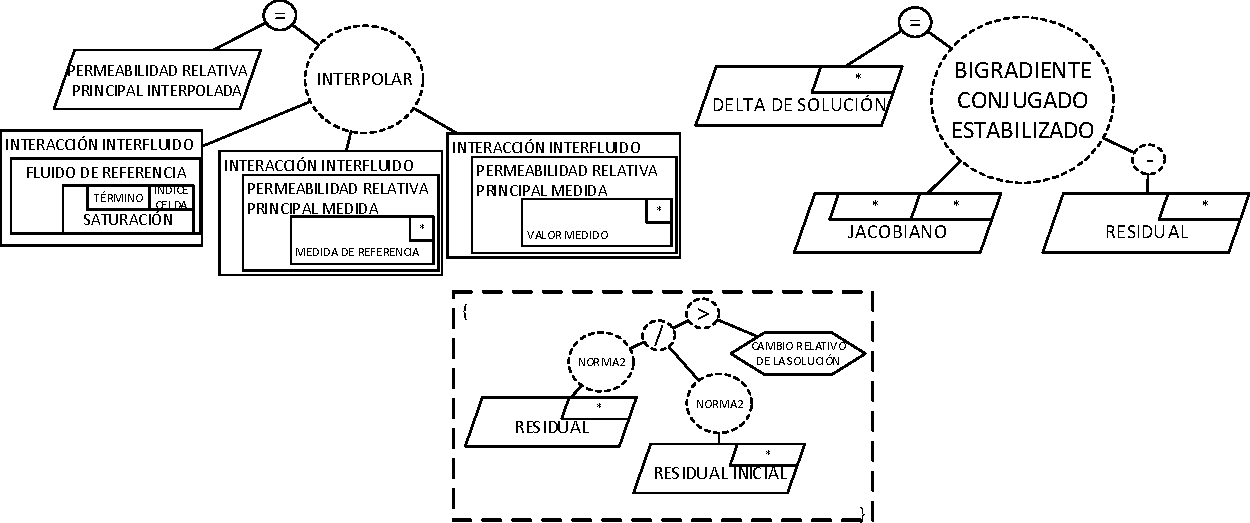
\includegraphics[scale=0.6]{Fig/OperadoresArreglos.pdf}%
	\caption[Ejemplos de operadores sobre arreglos.]{Ejemplos de operadores sobre arreglos. Los autores.} \label{fig:Operators}
\end{figure}

%\section{Conceptualization}\label{sec:Concepts}
\section{Conceptualización}\label{sec:Concepts}
En esta sección se explican los conceptos principales que resultan en la traducción de las ecuaciones algebraicas resultantes de la discretización del BOM extendido y las ecuaciones constitutivas usando el método de los volúmenes finitos. En la Figura \ref{fig:Concepts} se presentan los conceptos a explicar.

\begin{figure}[h]
	\centering%
	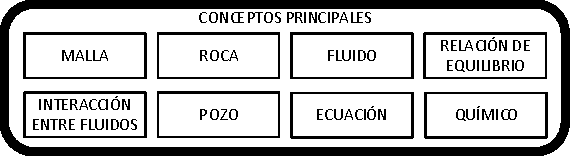
\includegraphics[width=0.9\linewidth]{Fig/Conceptos.pdf}%
	\caption[Conceptos principales en la simulación.]{Conceptos principales en la simulación. Los autores.} \label{fig:Concepts}
\end{figure}

%\subsection{Mesh}
\subsection{Malla}\label{subsec:PS_Mesh}
Al resolver el dominio espacial continuo como un conjunto discreto de celdas (discretizar el espacio), aparecen propiedades tales como los volúmenes de las celdas y el área de las caras. Este conjunto discreto de celdas es el que se denomina como ``malla''. A su vez, la celda es un conjunto discreto de caras que generan una superficie cerrada\footnote{En el caso tridimensional.}. Cada celda cuenta con una numeración, que sirve para identificar posiciones en el espacio y ubicar las vecindades correspondientes para el cálculo del flujo discretizado.\\

Una malla existe a partir de la conceptualización de los elementos emergentes en la discretización, que contiene todas las propiedades necesarias para generar el conjunto de celdas. Además, existe un actor ``geomodelador'' que se usa para definir el número de celdas en cada eje, sus espesores y topes tal como se presenta en  la Figura \ref{fig:Mesh}. Una vez se definen tales propiedades, la ``malla aparece'' en un proceso iterativo de creación de la cantidad de celdas y el respectivo cálculo de volúmenes, profundidades y numeración para cada una. Posteriormente, las caras se crean en otro proceso iterativo, conteniendo la información sobre las vecindades de cada celda, donde cada celda tiene un conjunto de caras\footnote{Es posible notar que la cara existente entre dos celdas vecinas se crea dos veces, una por cada celda.}.\\

\begin{figure}[h]
	\centering%
	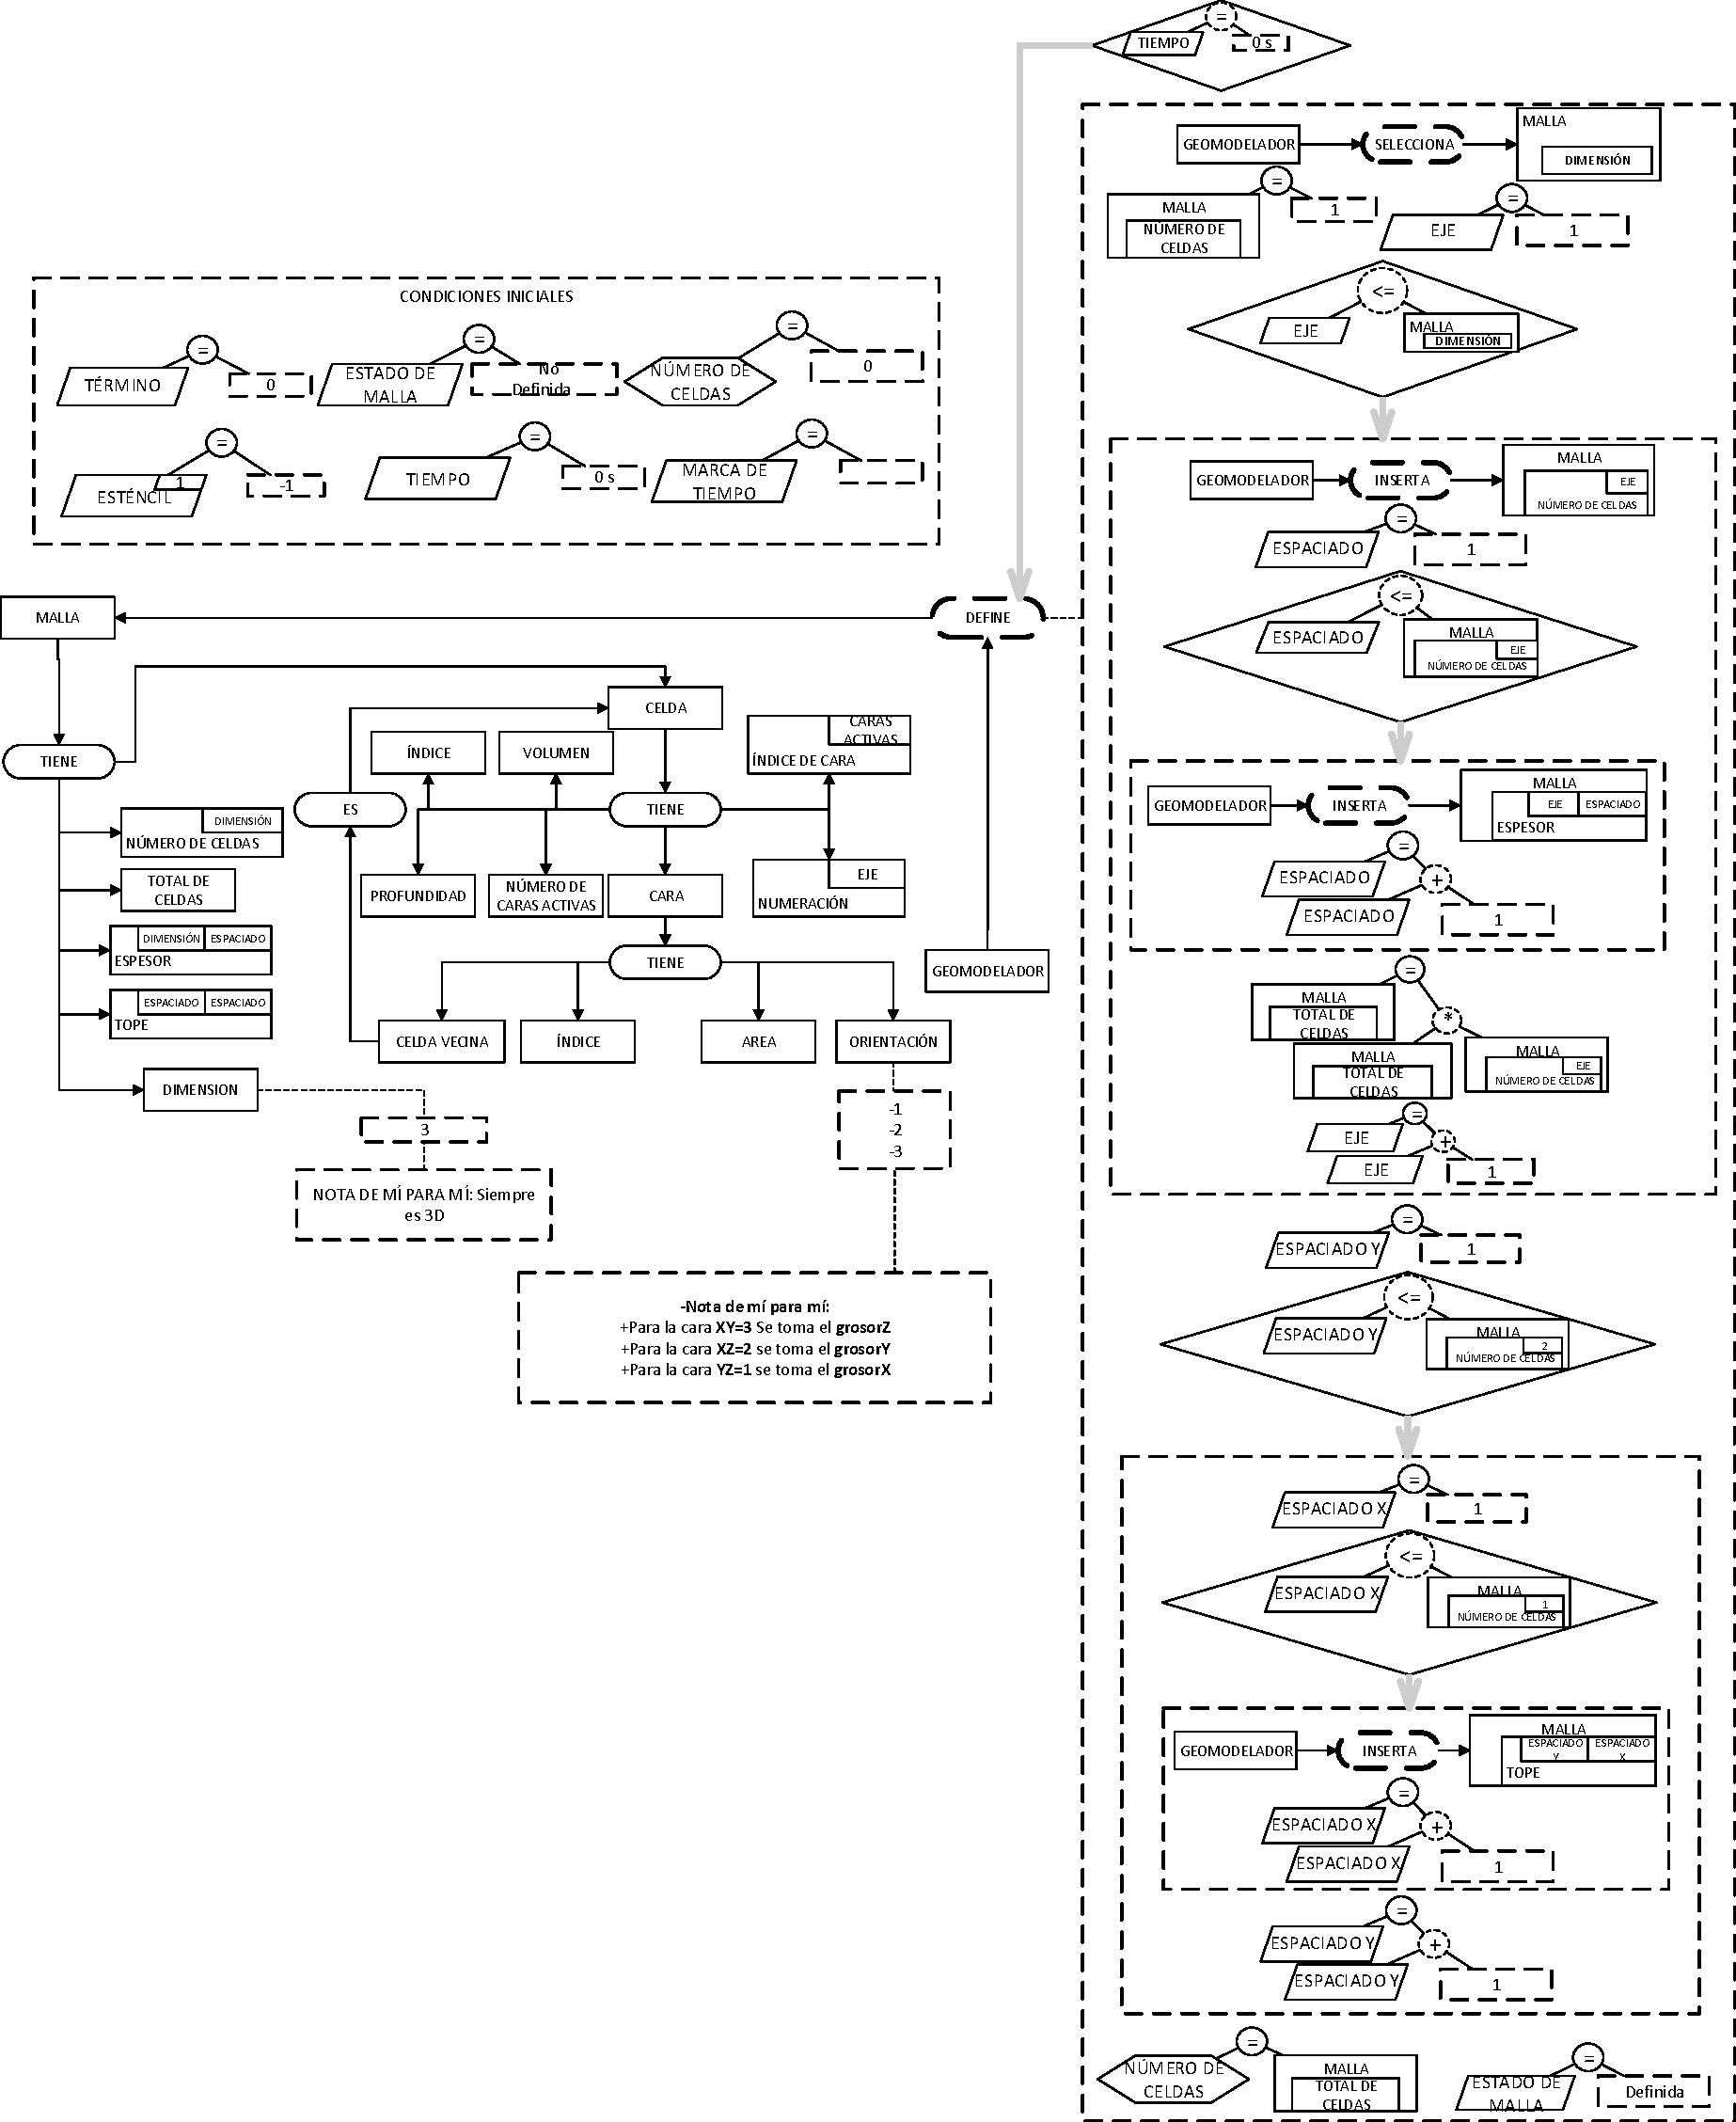
\includegraphics[width=\linewidth]{Fig/Mesh.pdf}%
	\caption[Definición de la malla.]{Definición de la malla. Los autores.} \label{fig:Mesh}
\end{figure}

%Este párrafo puede servirme más para la parte del evento.

\subsection{Malla aparece}\label{subsec:PS_MeshAppears}
El evento ``Malla aparece'' se dispara cuando el estado de la malla es ``Definida'', que sucede justo después de que el geomodelador defina la malla. En este evento, se desarrollan dos ciclos principales. El primer ciclo es anidado por cada eje coordenado, y en total se recorre el número de celdas a definir. En este ciclo, se calculan los volúmenes y profundidades de cada celda, además se asigna un índice único de celda y la numeración en cada eje $(x,y,z)$. La especificación del evento ``Malla Aparece'' se presenta en la Figura \ref{fig:MeshAppears}.\\

\begin{figure}[h]
	\centering%
	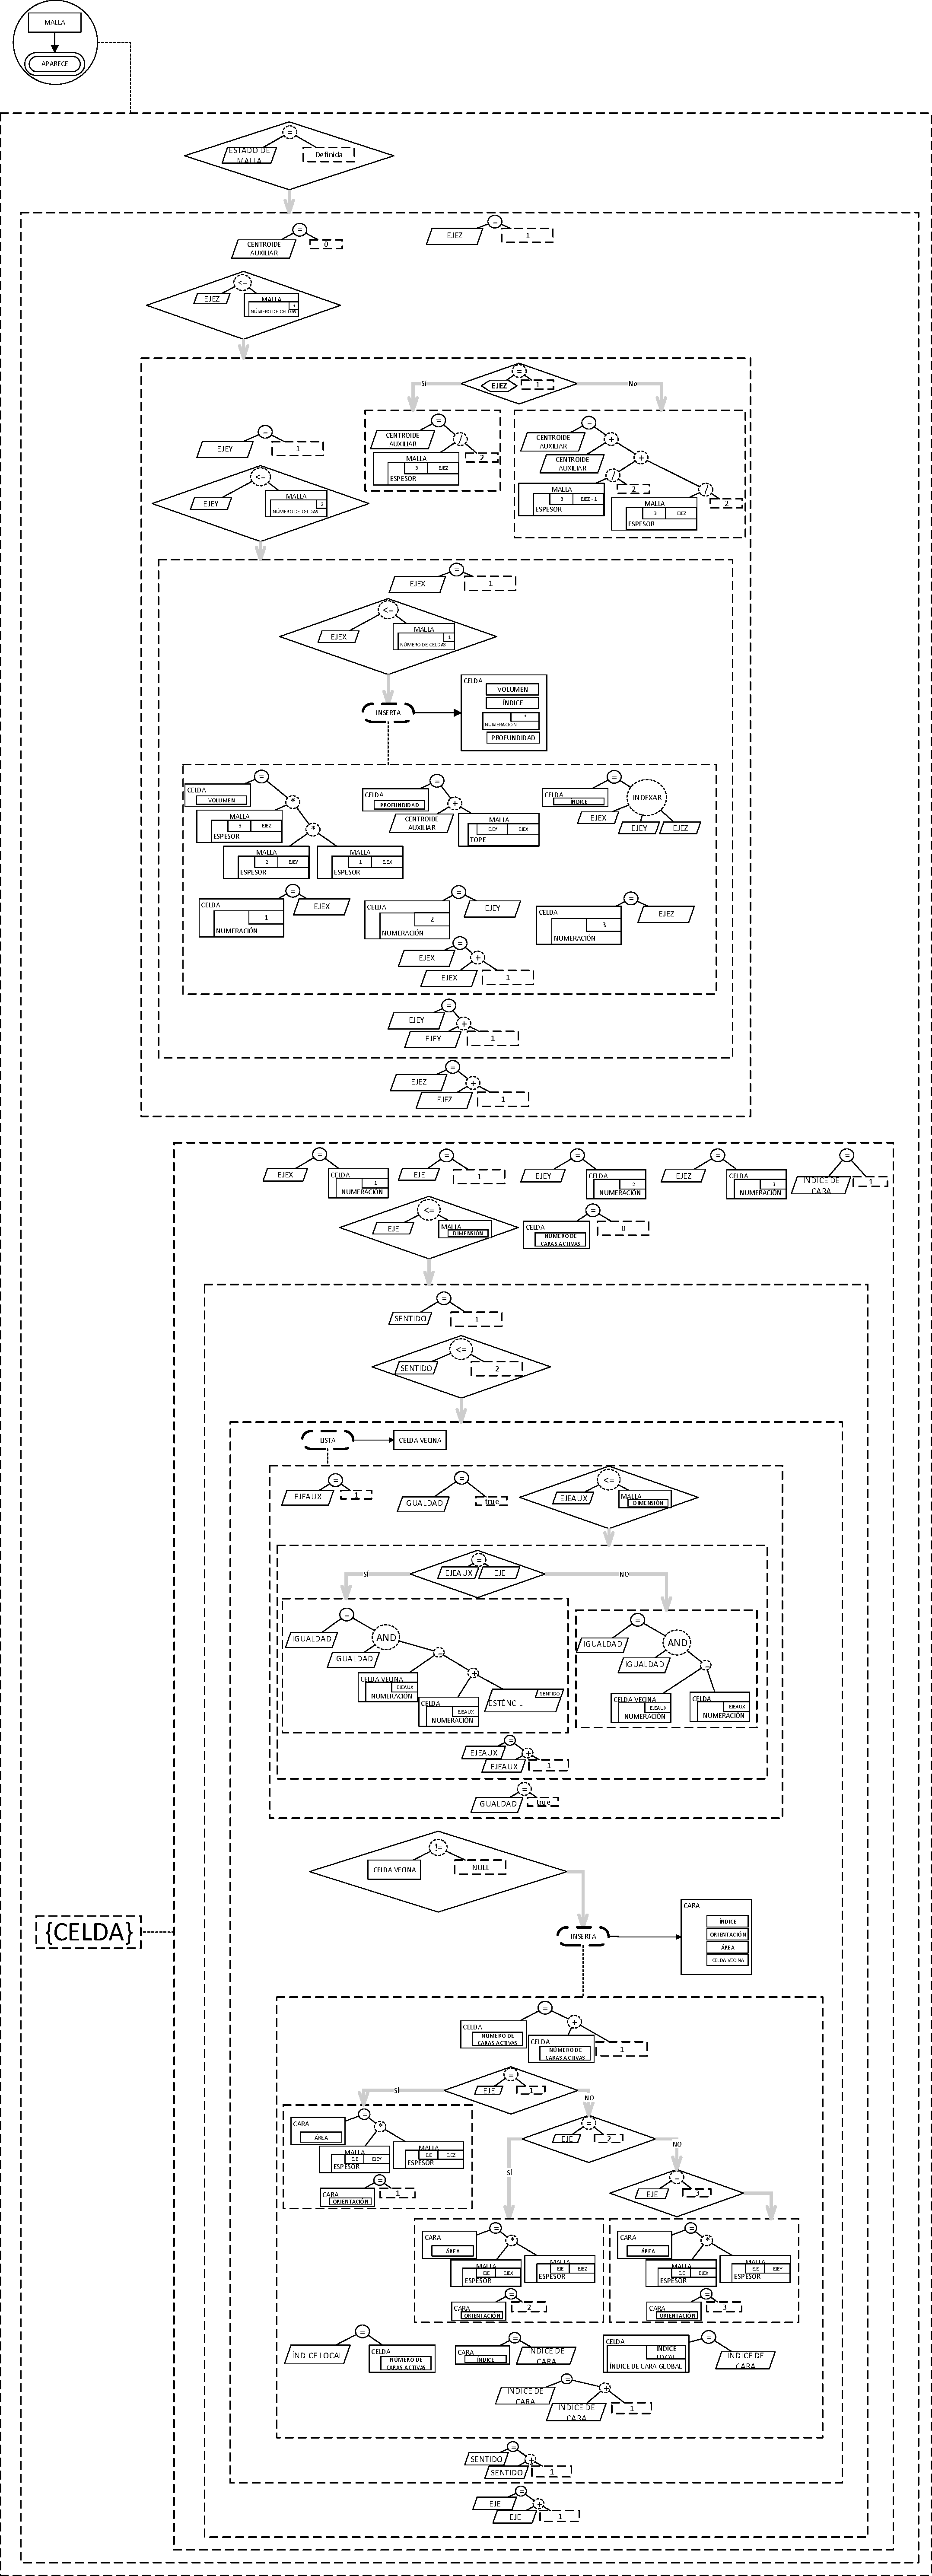
\includegraphics[height=0.9\textheight]{Fig/MallaAparece.pdf}%
	%\caption{Complete PS Representation for EOR Processes} \label{fig:PSComplete}
	\caption[Representación de la aparición de la Malla.]{Representación de la aparición de la Malla. Los autores.} \label{fig:MeshAppears}
\end{figure}

En el segundo ciclo principal, se itera sobre las celdas que se definen previamente y se calcula la conectividad, es decir la definición de caras. Para esto, se consulta la existencia de celdas adyacentes a la celda actual en todas las direcciones. Si existe una celda en alguna dirección, se crea y calcula su área y orientación. Adicionalmente, a la cara se le asigna un índice y también se le asigna la celda vecina. Es importante notar que cada celda almacena su conjunto de caras, por lo que las caras se duplican.
%We propose a representation of a mesh as a collection of cells which are represented likewise. collection of faces plus their respective attributes. This representation accounts for orthogonal cartesian meshes. Those are generated using the number of cells in each axis or direction, the thickness and top for each cell. Nevertheless, the thickness is only needed for the number of cells defined in every axis, because we work with regular meshes. Therefore the rest of the cells will have the same thickness.
%The top of the mesh is required for the first XY plane, and needs to be filled with the depths of each cell in that plane, the rest of the cells are calculated using the depth of the first plane.

%The representation stated for Mesh only accounts for orthogonal cartesian meshes, which can be generated with information about number of cells in each axis, their thickness and tops. A (The information above is inserted by a) Geomodeler with defines the mesh by inserting for each axis the number of cells and the thickness for cells in that direction. Once 

%\subsection{Rock}\label{sec:PS_Rock}
\subsection{Roca}\label{subsec:PS_Rock}

La especificación de la relación dinámica ``petrofísico caracteriza roca'' se especifica con la inserción de las condiciones iniciales de ``porosidad'' y ``permeabilidad absoluta'' para la roca que se asocia al yacimiento. Es posible notar que, estos atributos de la roca se representan como arreglos por la cantidad de términos, que se derivan de los pasos de tiempo, y la cantidad de celdas definidas en la malla. Adicionalmente, el petrofísico define la ``compresibilidad de poro'' y la ``presión de referencia'' a la que ésta se mide para el cálculo de la porosidad a los términos posteriores. El modelo incluye una única roca, a la cual se asignan todas las propiedades de cada una de las celdas. La caracterización de la roca se presenta en la Figura \ref{fig:Rock}.\\

\begin{figure}[h]
	\centering%
	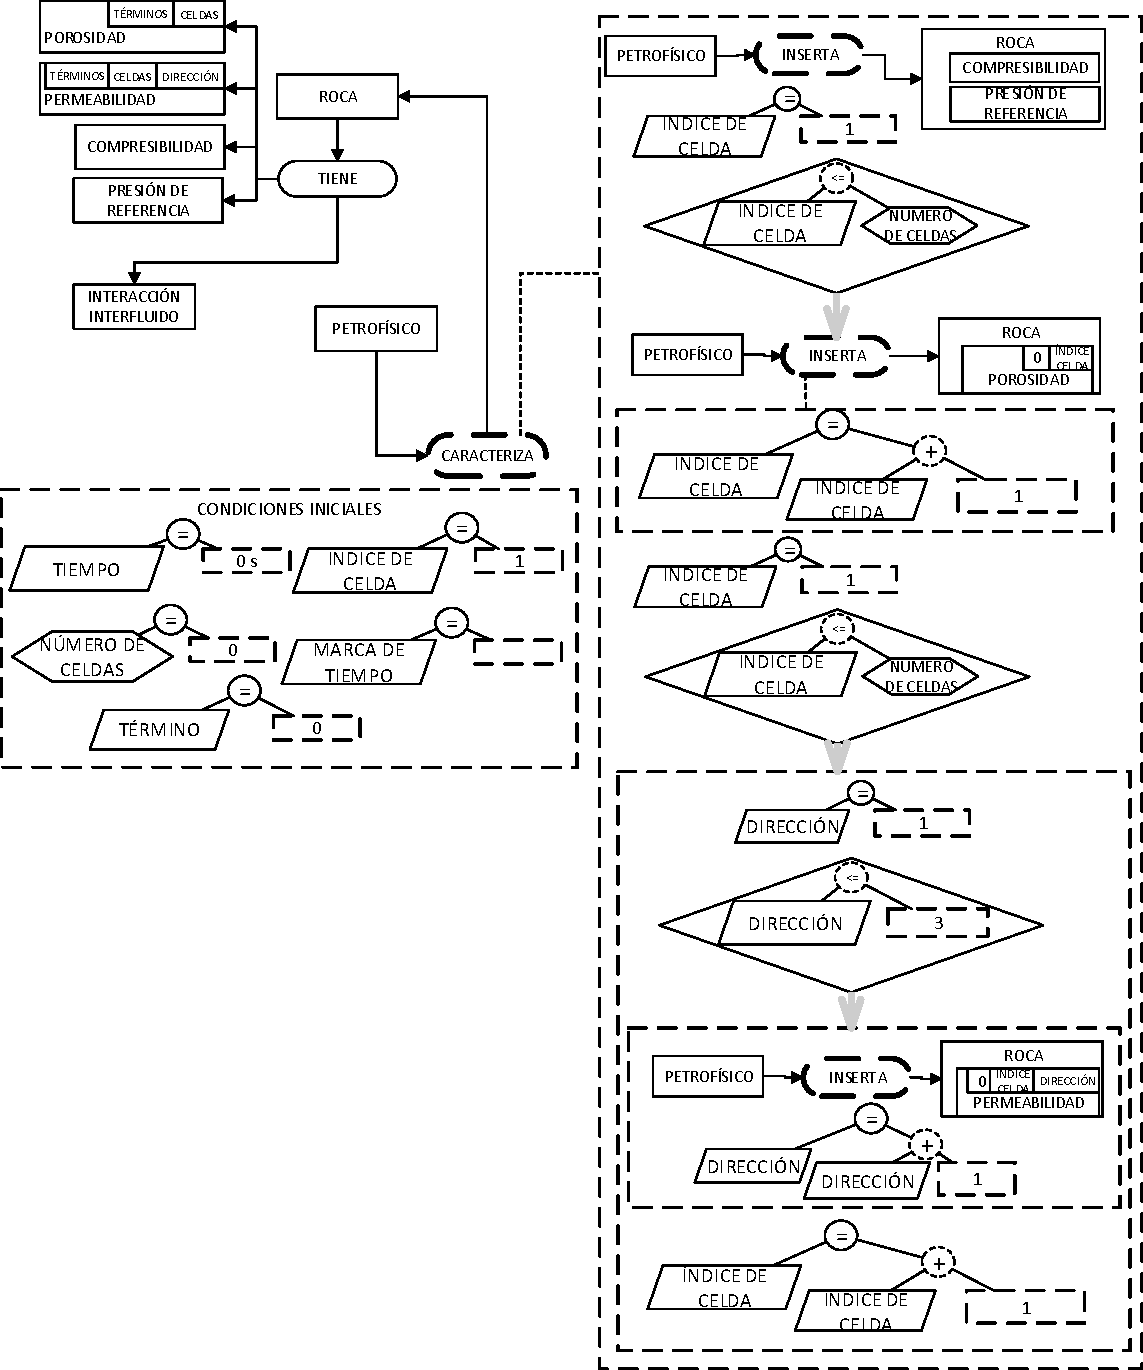
\includegraphics[width=0.7\linewidth]{Fig/Rock.pdf}%
	\caption[Caracterización de la Roca.]{Caracterización de la Roca. Los autores.} \label{fig:Rock}
\end{figure}

Se considera, además que la ``porosidad'' es función de la ``presión actual'' del sistema \citep{chen2007reservoir}. Y se aproxima en una celda $i$ como:

\begin{align}
	\label{ec:porosity}&\phi_{i} \approx \phi^{0}_{i}\left( 1 + C_{r} \left(P_{p,i} - P_{r}\right) \right)
\end{align}

donde $\phi^{0}_{i}$ corresponde a las condiciones iniciales de porosidad en la celda $i$, $C_{r}$ corresponde a la compresibilidad de la roca, $P_{r}$ a la presión de referencia para esa compresibilidad, y $P_{p,i}$ a la ``presión actual'', en la celda $i$, que se asocia con el fluido que tiene el atributo de principalidad. En la Figura \ref{fig:Porosity} se presenta el cálculo de porosidad para cada tiempo que se define como la función ``Calcular propiedad compresible'' en el EP.

\begin{figure}[h]
	\centering%
	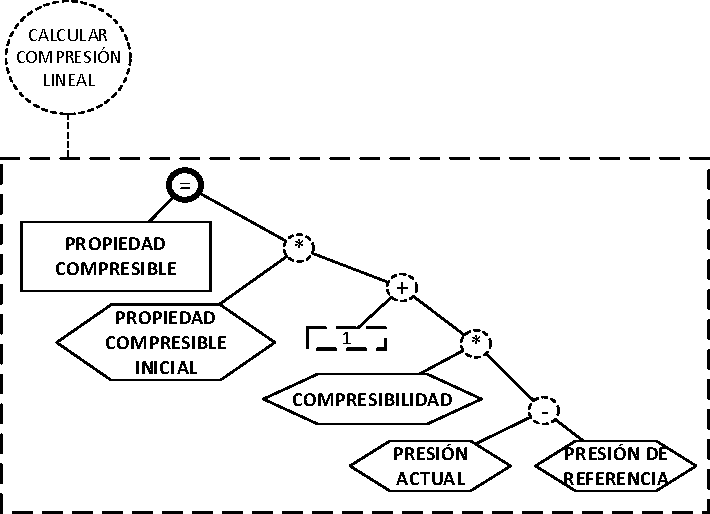
\includegraphics[scale=0.5]{Fig/PropiedadCompresible.pdf}%
	\caption[Función ``Calcular propiedad compresible''.]{Función ``Calcular propiedad compresible''. Los autores.} \label{fig:Porosity}
\end{figure}

%\subsection{Phase}\label{sec:PS_Phase}
\subsection{Fluido}\label{subsec:PS_Phase}

Los fluidos tienen propiedades que son funciones de su presión y saturación, las cuales, a su vez, son funciones del tiempo y del espacio. Así, todas las propiedades que se proponen en la conceptualización se representan como arreglos dependientes de la cantidad de términos y de la cantidad de celdas, tal como se presenta en la Figura \ref{fig:FluidProps}. La representación del fluido, su relación dinámica ``ingeniero de fluidos caracteriza fluido'' y su respectiva especificación se presentan en la Figura \ref{fig:Fluid}.\\

\begin{figure}[h]
	\centering%
	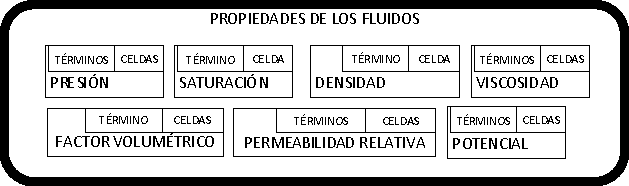
\includegraphics[width=0.9\linewidth]{Fig/PropiedadesDeFluidos.pdf}%
	\caption[Caracterización del fluido.]{Propiedades de los fluidos. Los autores.} \label{fig:FluidProps}
\end{figure}

\begin{figure}[h]
	\centering%
	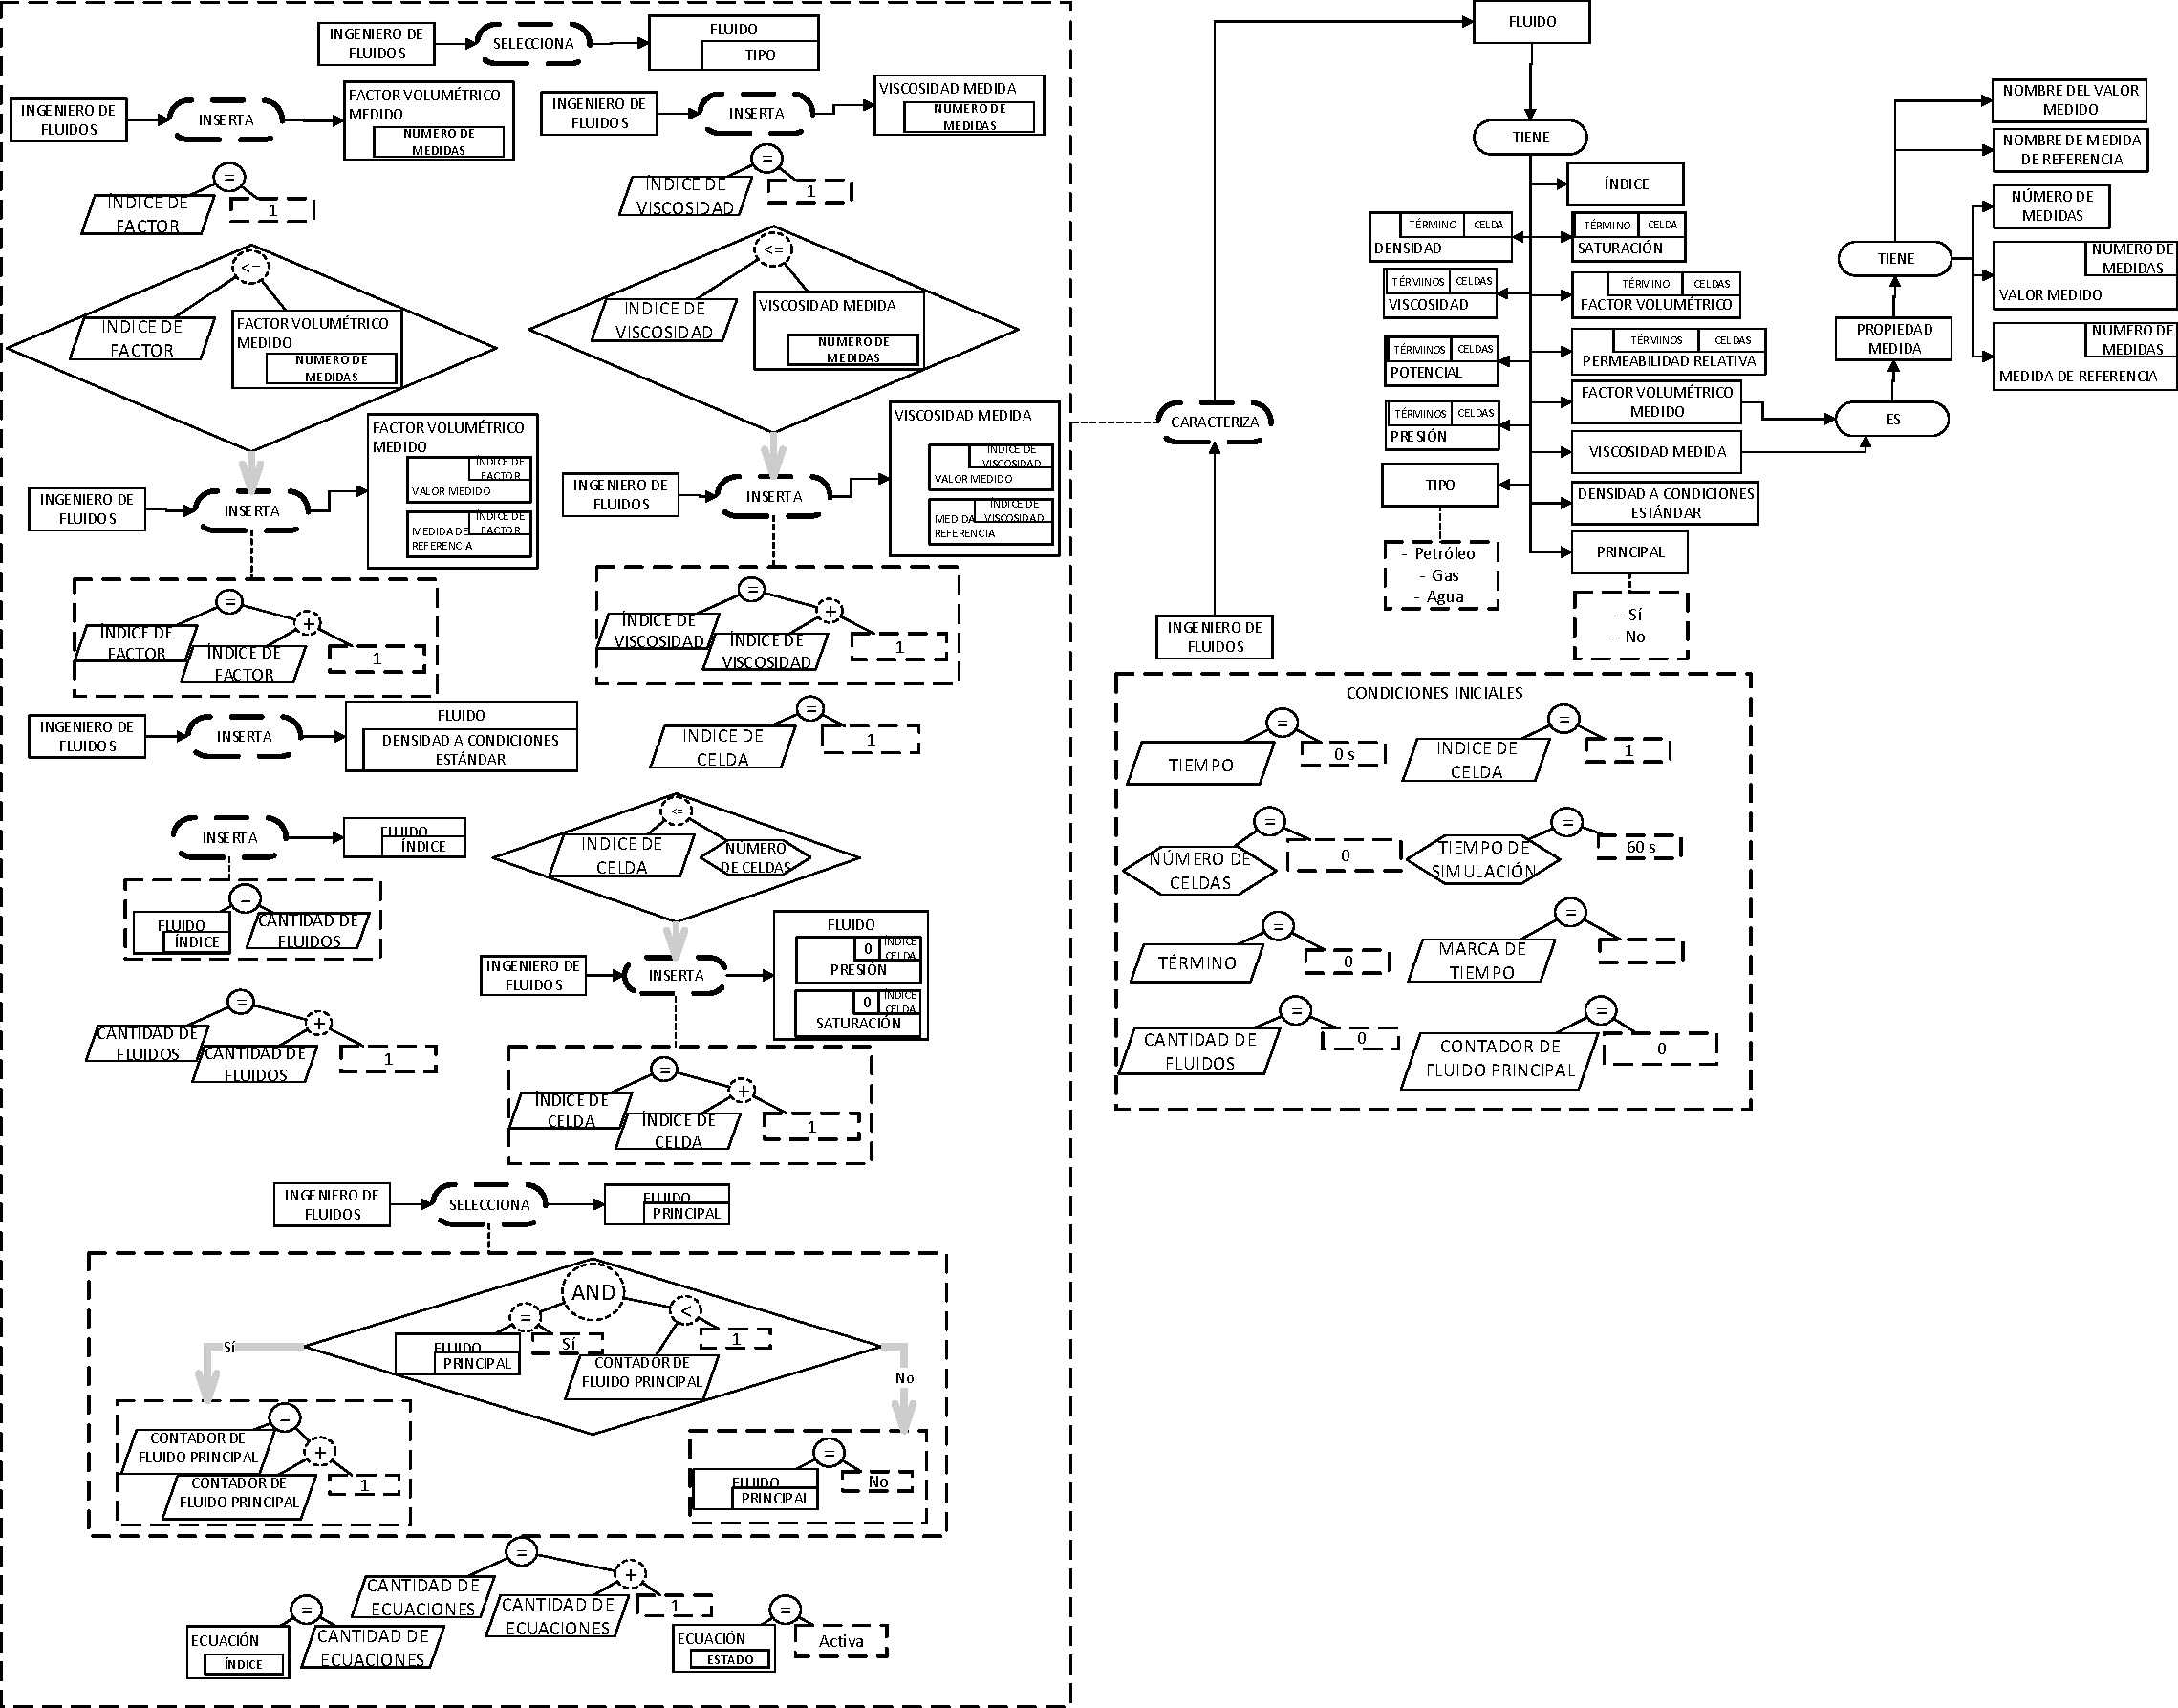
\includegraphics[width=0.9\linewidth]{Fig/Fluid.pdf}%
	\caption[Caracterización del fluido.]{Caracterización del fluido. Los autores.} \label{fig:Fluid}
\end{figure}

En pos de la generalidad, la ``viscosidad'' del ``fluido'' y su ``factor volumétrico'' se definen como funciones directas de su ``presión''. Con este fin, aparece el concepto de ``propiedad medida'', el cuál tiene una ``medida de referencia'' y un ``valor medido'' a esa referencia. Ambos son arreglos de la ``cantidad de medidas''. En la Figura \ref{fig:Fluid} también es posible ver que el fluido tiene una ``viscosidad medida'' y un ``factor volumétrico medido''. Esto permite calcular de manera general estas propiedades, independientemente del fluido, como una interpolación en el conjunto de medidas a la presión del fluido correspondiente. El ingeniero de fluidos inserta la viscosidad medida y el factor volumétrico medido cuando ``caracteriza el fluido''. \\

Es importante notar también, que el fluido tiene un ``tipo'' y un atributo de tipo lógico ``principal''. El tipo del fluido puede ser ``petróleo'', ``gas'' o ``agua''. Sin embargo, el fluido cuyo atributo principal sea ``sí'' o ``\textit{true}'', incluye su ``presión'' en su respectiva ecuación. Los demás fluidos incluyen su ``saturación''. Esto permite tener flexibilidad en el modelado de casos de estudio en el que alguno de los fluidos no exista.
 
%\subsection{Inter-phase interaction}\label{sec:PS_Interphase}
\subsection{Interacción entre fluidos}\label{subsec:PS_Interphase}
%
% Qué debo mencionar acá:
% Este concepto me relaciona la presión del fluido principal con la del de referencia (Presión Capilar)
% Se espera que existan exactamente 2 para un Black Oil Model y en caso de un sistema bifásico sólo una
% Se generaliza cálculo de presiones capilares a partir de la existencia de un fluido mojante y uno no mojante.
% Se espera que uno de los dos (El fluido Mojante o el no Mojante) sea el fluido de referencia
% Todos los fluidos son claves foráneas a un fluido (No es que existan fluidos adicionales)
% Se asume que el fluido principal también es el que tiene los dos "contactos" - Hay que hablar de contactos en la conceptualización
% Las permeabilidades relativas tanto de referencia como principal y la presión capilar se interpolan a la saturación del fluido de referencia (Se verá luego).

%%%%%%%%%%%%%%%%%%%%%%%%%%%%%%%%%%%%%%%%%%%%%%%%%%%%%%%%%%%%%%%%%%%%%%%%%%%%%%%%%%%%%%%%%%%%%%%%%%%%%%%%%%%%%%%%%%%%%%%%%%%%%%%%%%%%%%%%%%%%%%%%%%%%%%%%%%%%%%%%%%%%%%%%%%%%%%%%
%NOTA: Es posible que este párrafo me sirva más para la parte de conceptualización de las Krs
%%%%%%%%%%%%%%%%%%%%%%%%%%%%%%%%%%%%%%%%%%%%%%%%%%%%%%%%%%%%%%%%%%%%%%%%%%%%%%%%%%%%%%%%%%%%%%%%%%%%%%%%%%%%%%%%%%%%%%%%%%%%%%%%%%%%%%%%%%%%%%%%%%%%%%%%%%%%%%%%%%%%%%%%%%%%%%%%
Las interacciones entre fluidos se proponen como una generalización de los contactos entre fluidos (véase Subsección \ref{subsec:Krs}). En el caso del modelo BOM, se deben especificar dos: los contactos gas-aceite y aceite-agua. En este concepto, se relacionan directamente las dependencias de la ``permeabilidad relativa del fluido principal'' con su respectivo ``fluido de referencia'' en el contacto. Además, para el fluido cuya incógnita es la saturación, se relaciona la presión del fluido principal con su respectiva ``presión capilar'', con el fin de calcular la presión faltante. Para esto, es necesario saber de antemano cuál es el ``fluido mojante'' y cuál es el ``fluido no mojante''. Adicionalmente, todas las propiedades que se mencionan son ``propiedades medidas'' que se calculan a la saturación del fluido de referencia. En la Figura \ref{fig:Contact} se presenta la representación propuesta para las interacciones entre fluidos.\\

\begin{figure}[h]
	\centering%
	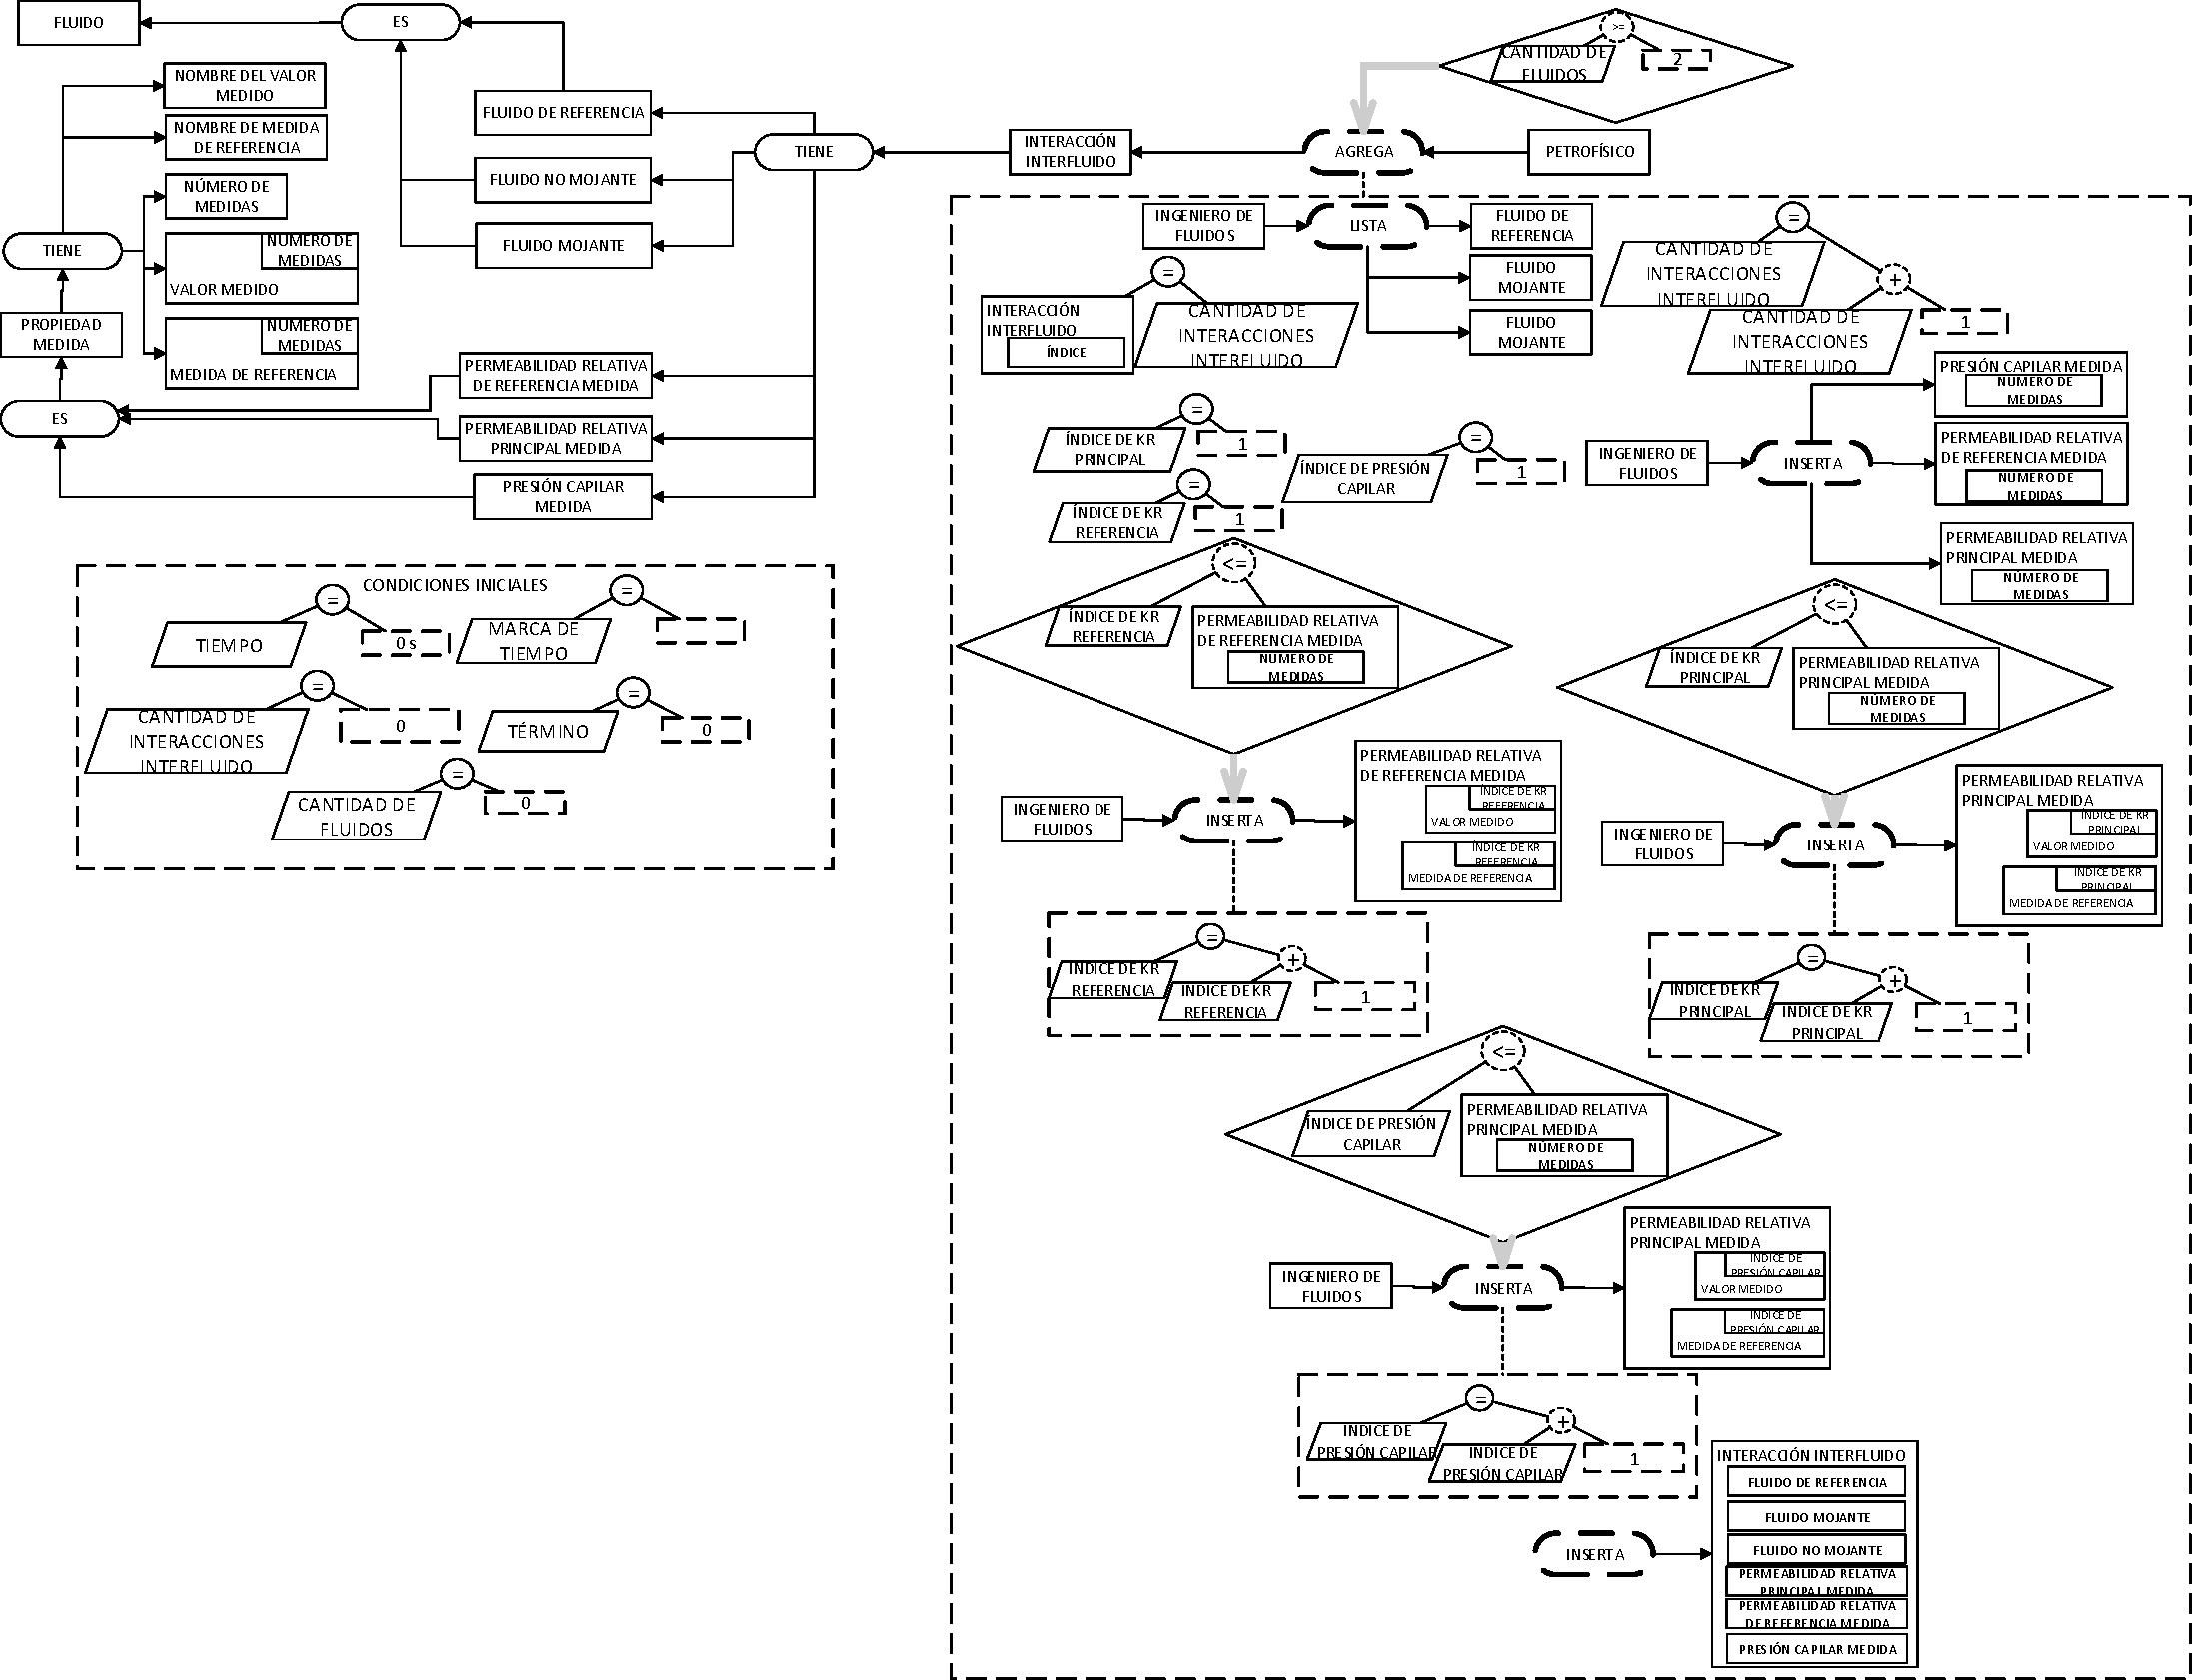
\includegraphics[width=0.9\linewidth]{Fig/Interphase.pdf}%
	\caption[Adición de Interacción entre fluidos.]{Adición de Interacción entre fluidos. Los autores.} \label{fig:Contact}
\end{figure}
%este concepto me relaciona un fluido de referencia, que se espera diferente del fluido con la propiedad de ser ``Principal'' y es respecto al cual se interpolarán las permeabilidades relativas, tanto propias como del fluido principal.

La permeabilidad relativa conjunta $k_{rp}$, es decir, la del fluido principal considerando todos sus contactos, se calcula usando la interpolación de \cite{Baker1988}, tal como se presenta en la Ecuación \ref{ec:Baker}. Se define la saturación del fluido de referencia como $S_{r}$, la saturación irreducible del fluido como $S_{rc}$, y la permeabilidad relativa del fluido principal al fluido de referencia como $k_{rpr}$. Así, la interpolación de \cite{Baker1988}, en términos de las interacciones entre fluidos $in$, queda:

\begin{align}
	\label{ec:IntBaker}&k_{rp} = \frac{\sum_{in \in I}\left[\left(S_{r,in} - S_{rc,in}\right)k_{rpr,in}\left(S_{r,in}\right)\right]}{\sum_{in \in I}\left[\left(S_{r,in} - S_{rc,in}\right)\right]}
\end{align}

La representación de la interpolación de \cite{Baker1988} en la Ecuación \ref{ec:IntBaker}, se ilustra en la Figura \ref{fig:Baker}.

\begin{figure}[h]
	\centering%
	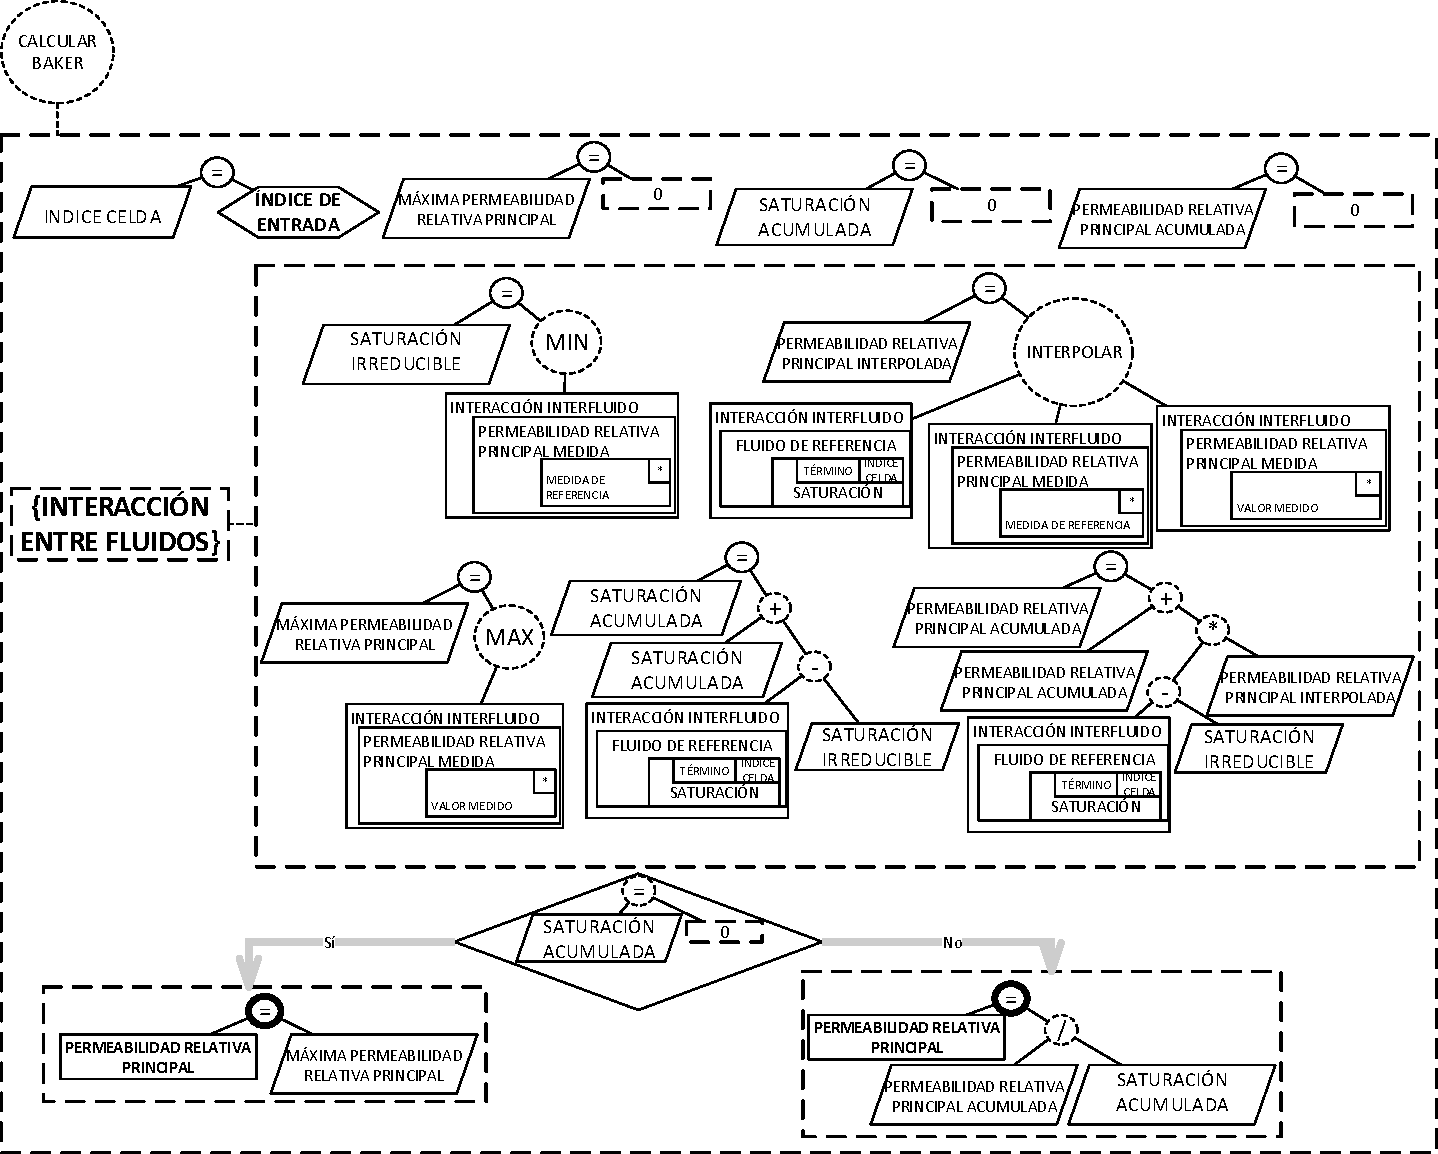
\includegraphics[width=0.9\linewidth]{Fig/Baker.pdf}%
	\caption[Función ``Calcular Baker''.]{Función ``Calcular Baker''. Los autores.} \label{fig:Baker}
\end{figure}

%\subsection{Equilibrium Relation}\label{sec:PS_Equilibrium}
\subsection{Relación de Equilibrio}\label{subsec:PS_Equilibrium}
En las ecuaciones del BOM se considera existencia de masa de gas en el aceite ($R_{s}$ o gas disuelto), y, en el caso del BOM extendido, la de aceite en el gas ($R_{v}$ o aceite volatilizado). En el concepto ``Relación de equilibrio'', se generaliza la existencia de masa de un fluido dentro de otro fluido con un ``coeficiente de partición''. Se postula, también, que existe un ``fluido aportante'' y un ``fluido receptor'', tal como se ve en la Figura \ref{fig:EqRelation}. El coeficiente de partición cumple la mismas condiciones de la viscosidad o el factor volumétrico del fluido. Además, la relación de equilibrio tiene un ``coeficiente de partición medido''.\\

\begin{figure}[h]
	\centering%
	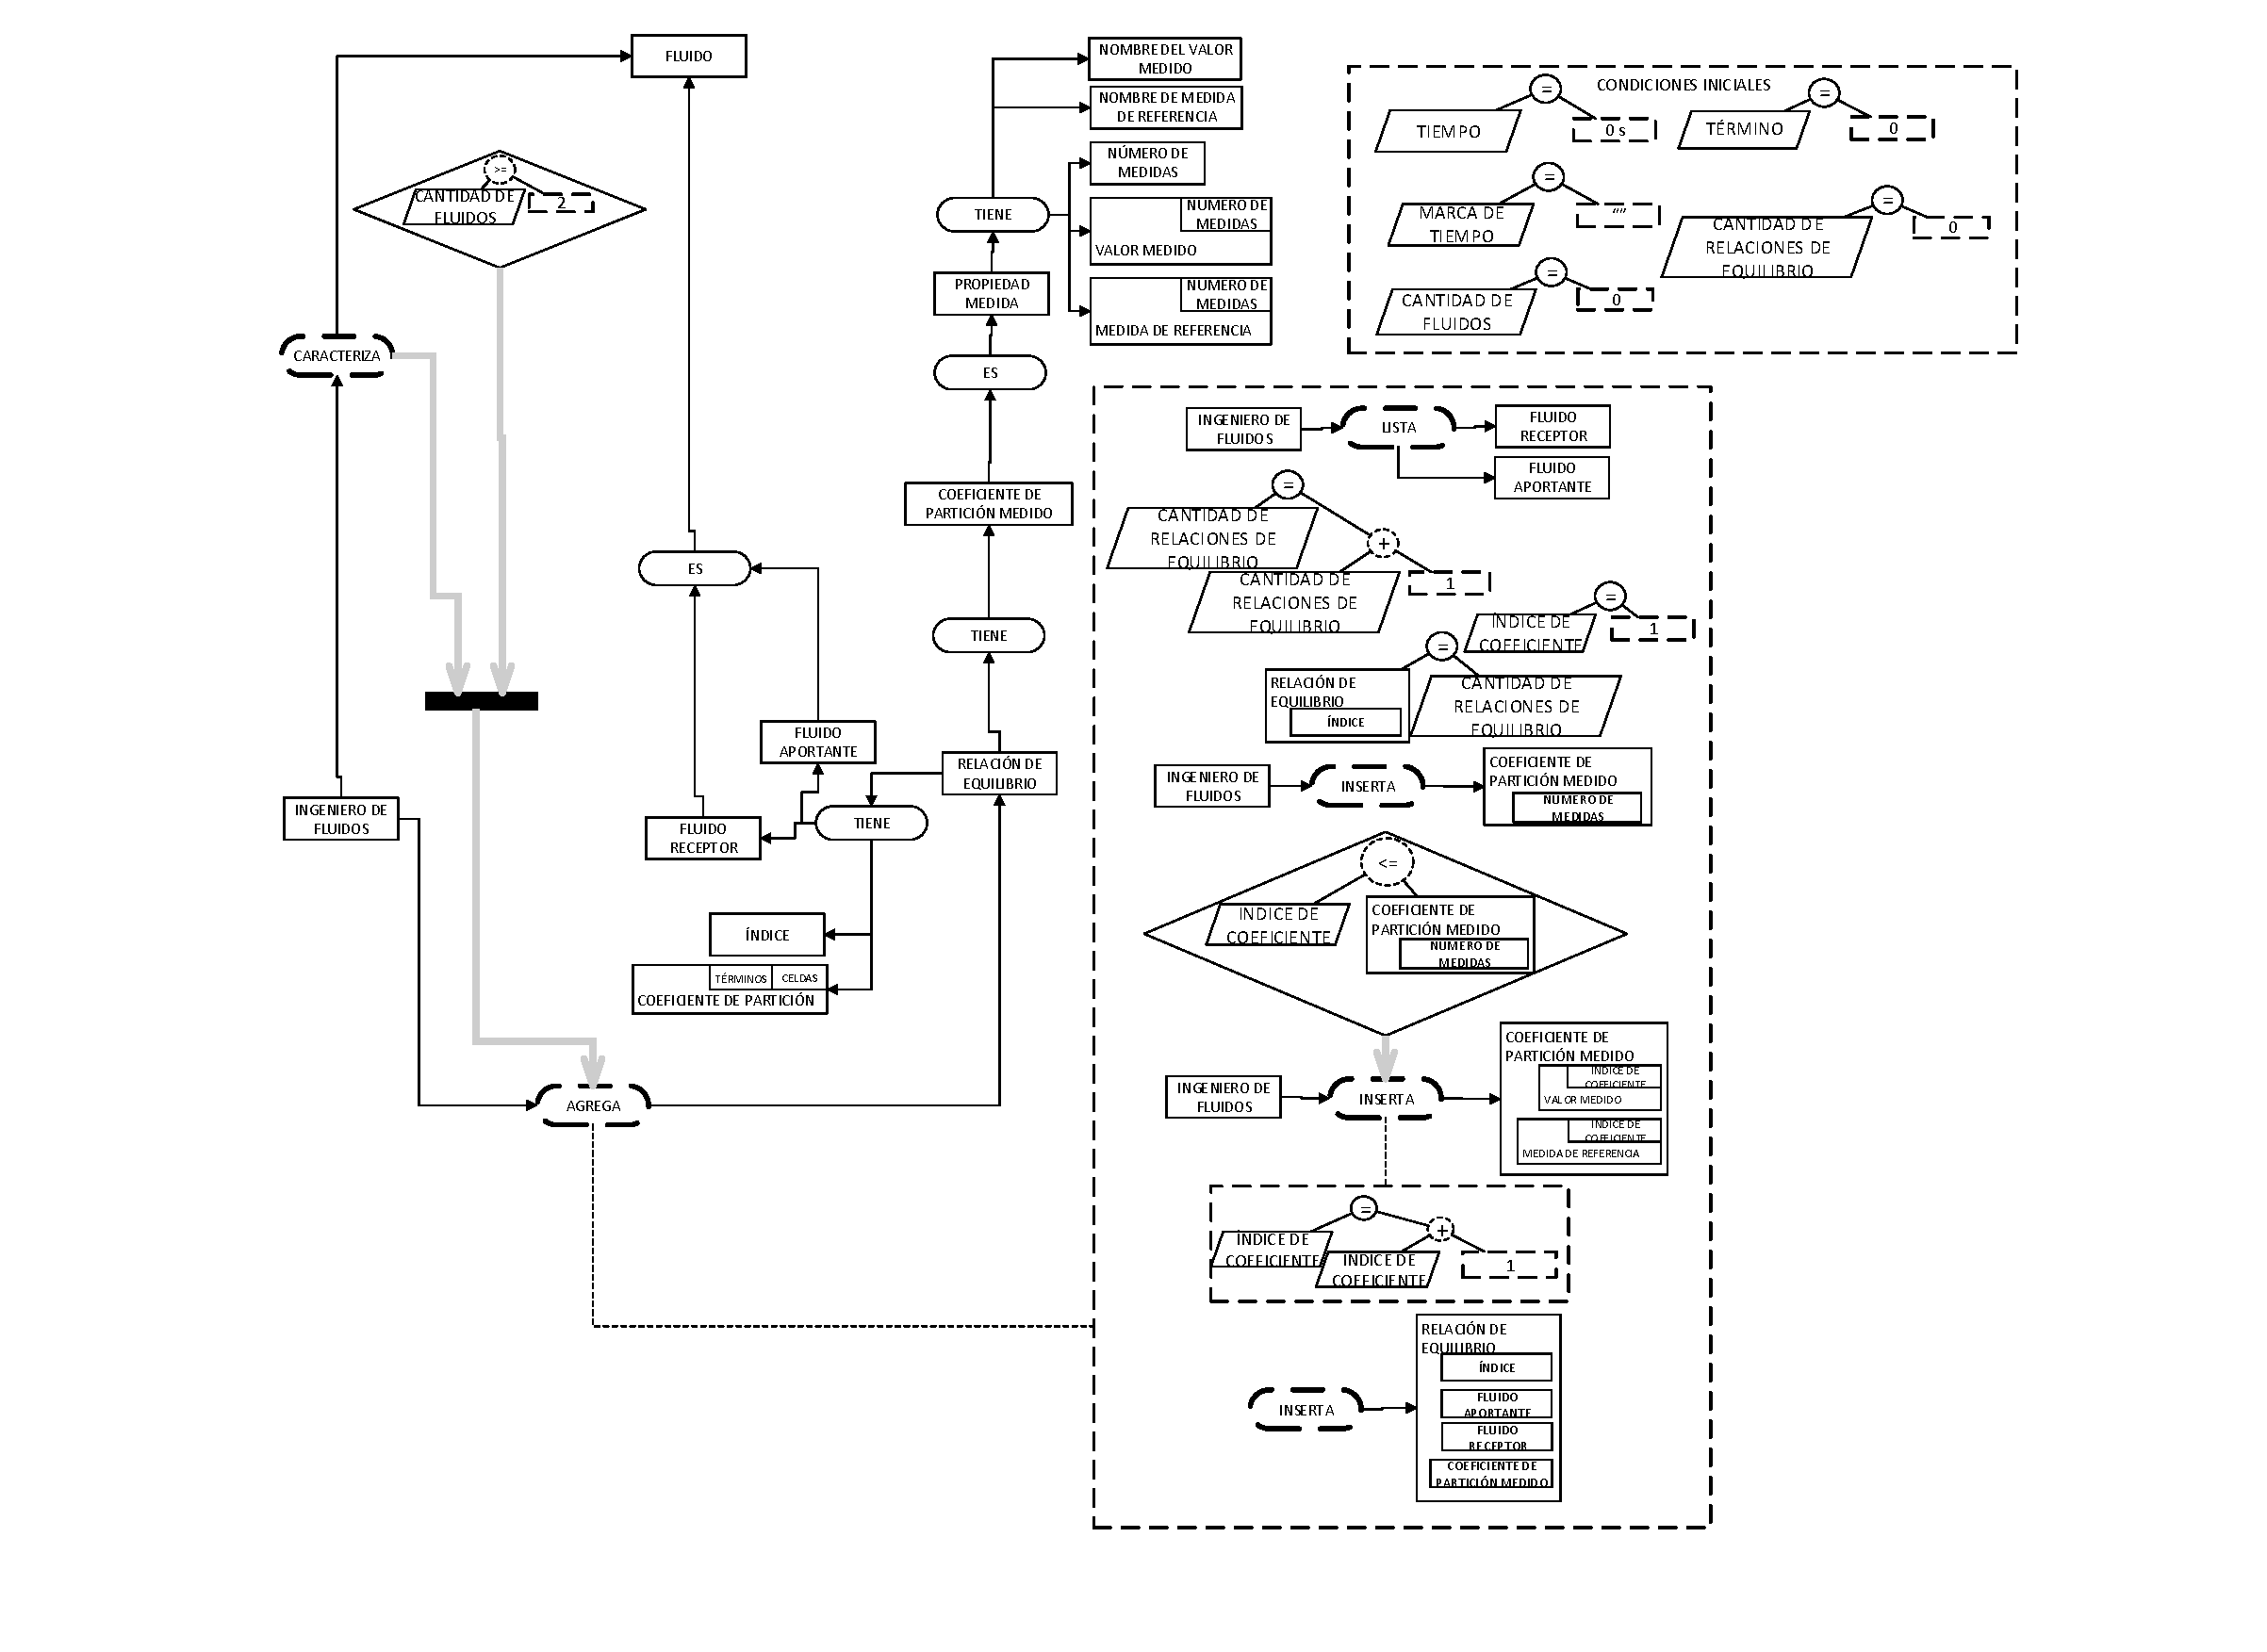
\includegraphics[width=0.9\linewidth]{Fig/Equilibrium.pdf}%
	\caption[Adición de Relaciones de equilibrio.]{Adición de Relaciones de equilibrio. Los autores.} \label{fig:EqRelation}
\end{figure}

Tal definición de las relaciones de equilibrio tiene implicaciones en el cálculo de la densidad de los fluidos, de la acumulación y del flujo. En el cálculo de densidad de un fluido, se debe considerar la masa de cualquier otro fluido que esté presente dentro del mismo. Así, en el caso concreto del BOM, existe gas en el aceite, y en el BOM Extendido,
aceite en el gas. Se recuerdan los cálculos de densidades en \ref{ec:oildensity}, \ref{ec:gasdensity}, \ref{ec:watdensity} como se explican en la Subsección \ref{subsec:BOM}:

\begin{align*}
&\rho_{o} = \frac{\rho_{o,sc} + R_{s}\rho_{g,sc}}{B_{o}}\\
&\rho_{g} = \frac{\rho_{g,sc} + R_{v}\rho_{o,sc}}{B_{g}}\\
&\rho_{w} = \frac{\rho_{w,sc}}{B_{w}}
\end{align*}

En las relaciones de equilibrio se propone que puede existir cualquier transferencia de masa en equilibrio de un fluido a otro. Por tanto, la densidad de un fluido debe calcularse con los aportes de densidad de los fluidos receptores por todas las relaciones de equilibrio en las que éste es el fluido aportante. Tal como se presenta en:

\begin{align}
	\label{ec:generaldensity}&\rho_{a} = \dfrac{\rho_{a,sc} + \sum_{r \in R}\left[\chi_{a,r}\rho_{r,sc}\right]}{B_{a}}
\end{align}

donde $\chi$ es el coeficiente de partición en el que se relacionan el fluido aportante $a$, y el fluido receptor $r$, y $R$ el conjunto de relaciones de equilibrio en las que $a$ es el fluido aportante. Se destaca que $\chi$ es una relación volumétrica a condiciones estándar y es función de la presión del fluido aportante $a$ ($\chi_{a,r}\left(P_{a}\right)$).\\

Para el cálculo del flujo y de la acumulación, se recuerdan las Ecuaciones que se discretizan del BOM Extendido \ref{ec:aceiteDiscretizacion}, \ref{ec:gasDiscretizacion}, \ref{ec:aguaDiscretizacion} en las que se considera la existencia de gas disuelto ($R_{s}$) y aceite volatilizado ($R_v$), como se muestra en la Subsección \ref{subsec:BOM}. Éstas ecuaciones se generalizan para un fluido receptor $r$ arbitrario como sigue:

\begin{align}
	\label{ec:acumulacion_releq}\text{Acumulación: }&\frac{|\Omega_{i}|}{\Delta t}\left[ \phi_{i} \left( \frac{S_{r,i}}{B_{r,i}} + \sum_{a \in R}\frac{\chi_{a,r,i}S_{a,i}}{B_{a,i}}\right)\right]^{n+1}_{n}\\
	\label{ec:flujo_releq}\text{Flujo: }&\sum_{c \in S}\left[ T^{n+1}_{r,c} \Delta{\Phi_{r,c}^{n+1}} + \sum_{a \in R}\chi_{a,r,c} T^{n+1}_{a,c} \Delta{\Phi_{a,c}^{n+1}} \right]
\end{align}

%\subsection{Component}\label{sec:PS_Component} % This could be changed to Chemical
%\subsection{Well}\label{sec:PS_Well}
\subsection{Pozo}\label{subsec:PS_Well}
Se proponen los pozos, de manera análoga a la malla, como un conjunto de ``perforados'' que a su vez tienen atributos adicionales como lo son la ``presión de fondo'' y el ``caudal''. Estos pozos, tienen una caracterización distinta según el tipo, sea productor o inyector. Además, es posible notar que el ``pozo'' es un concepto abstracto, de cuál se instancia uno de los dos tipos. Más aún, los perforados dependerán del tipo de pozo, siendo estos también abstractos, con sus respectivos tipos ``perforado inyector'' o ``perforado productor''. En la Figura \ref{fig:Well} se presenta la representación de los pozos.\\

\begin{figure}[h]
	\centering%
	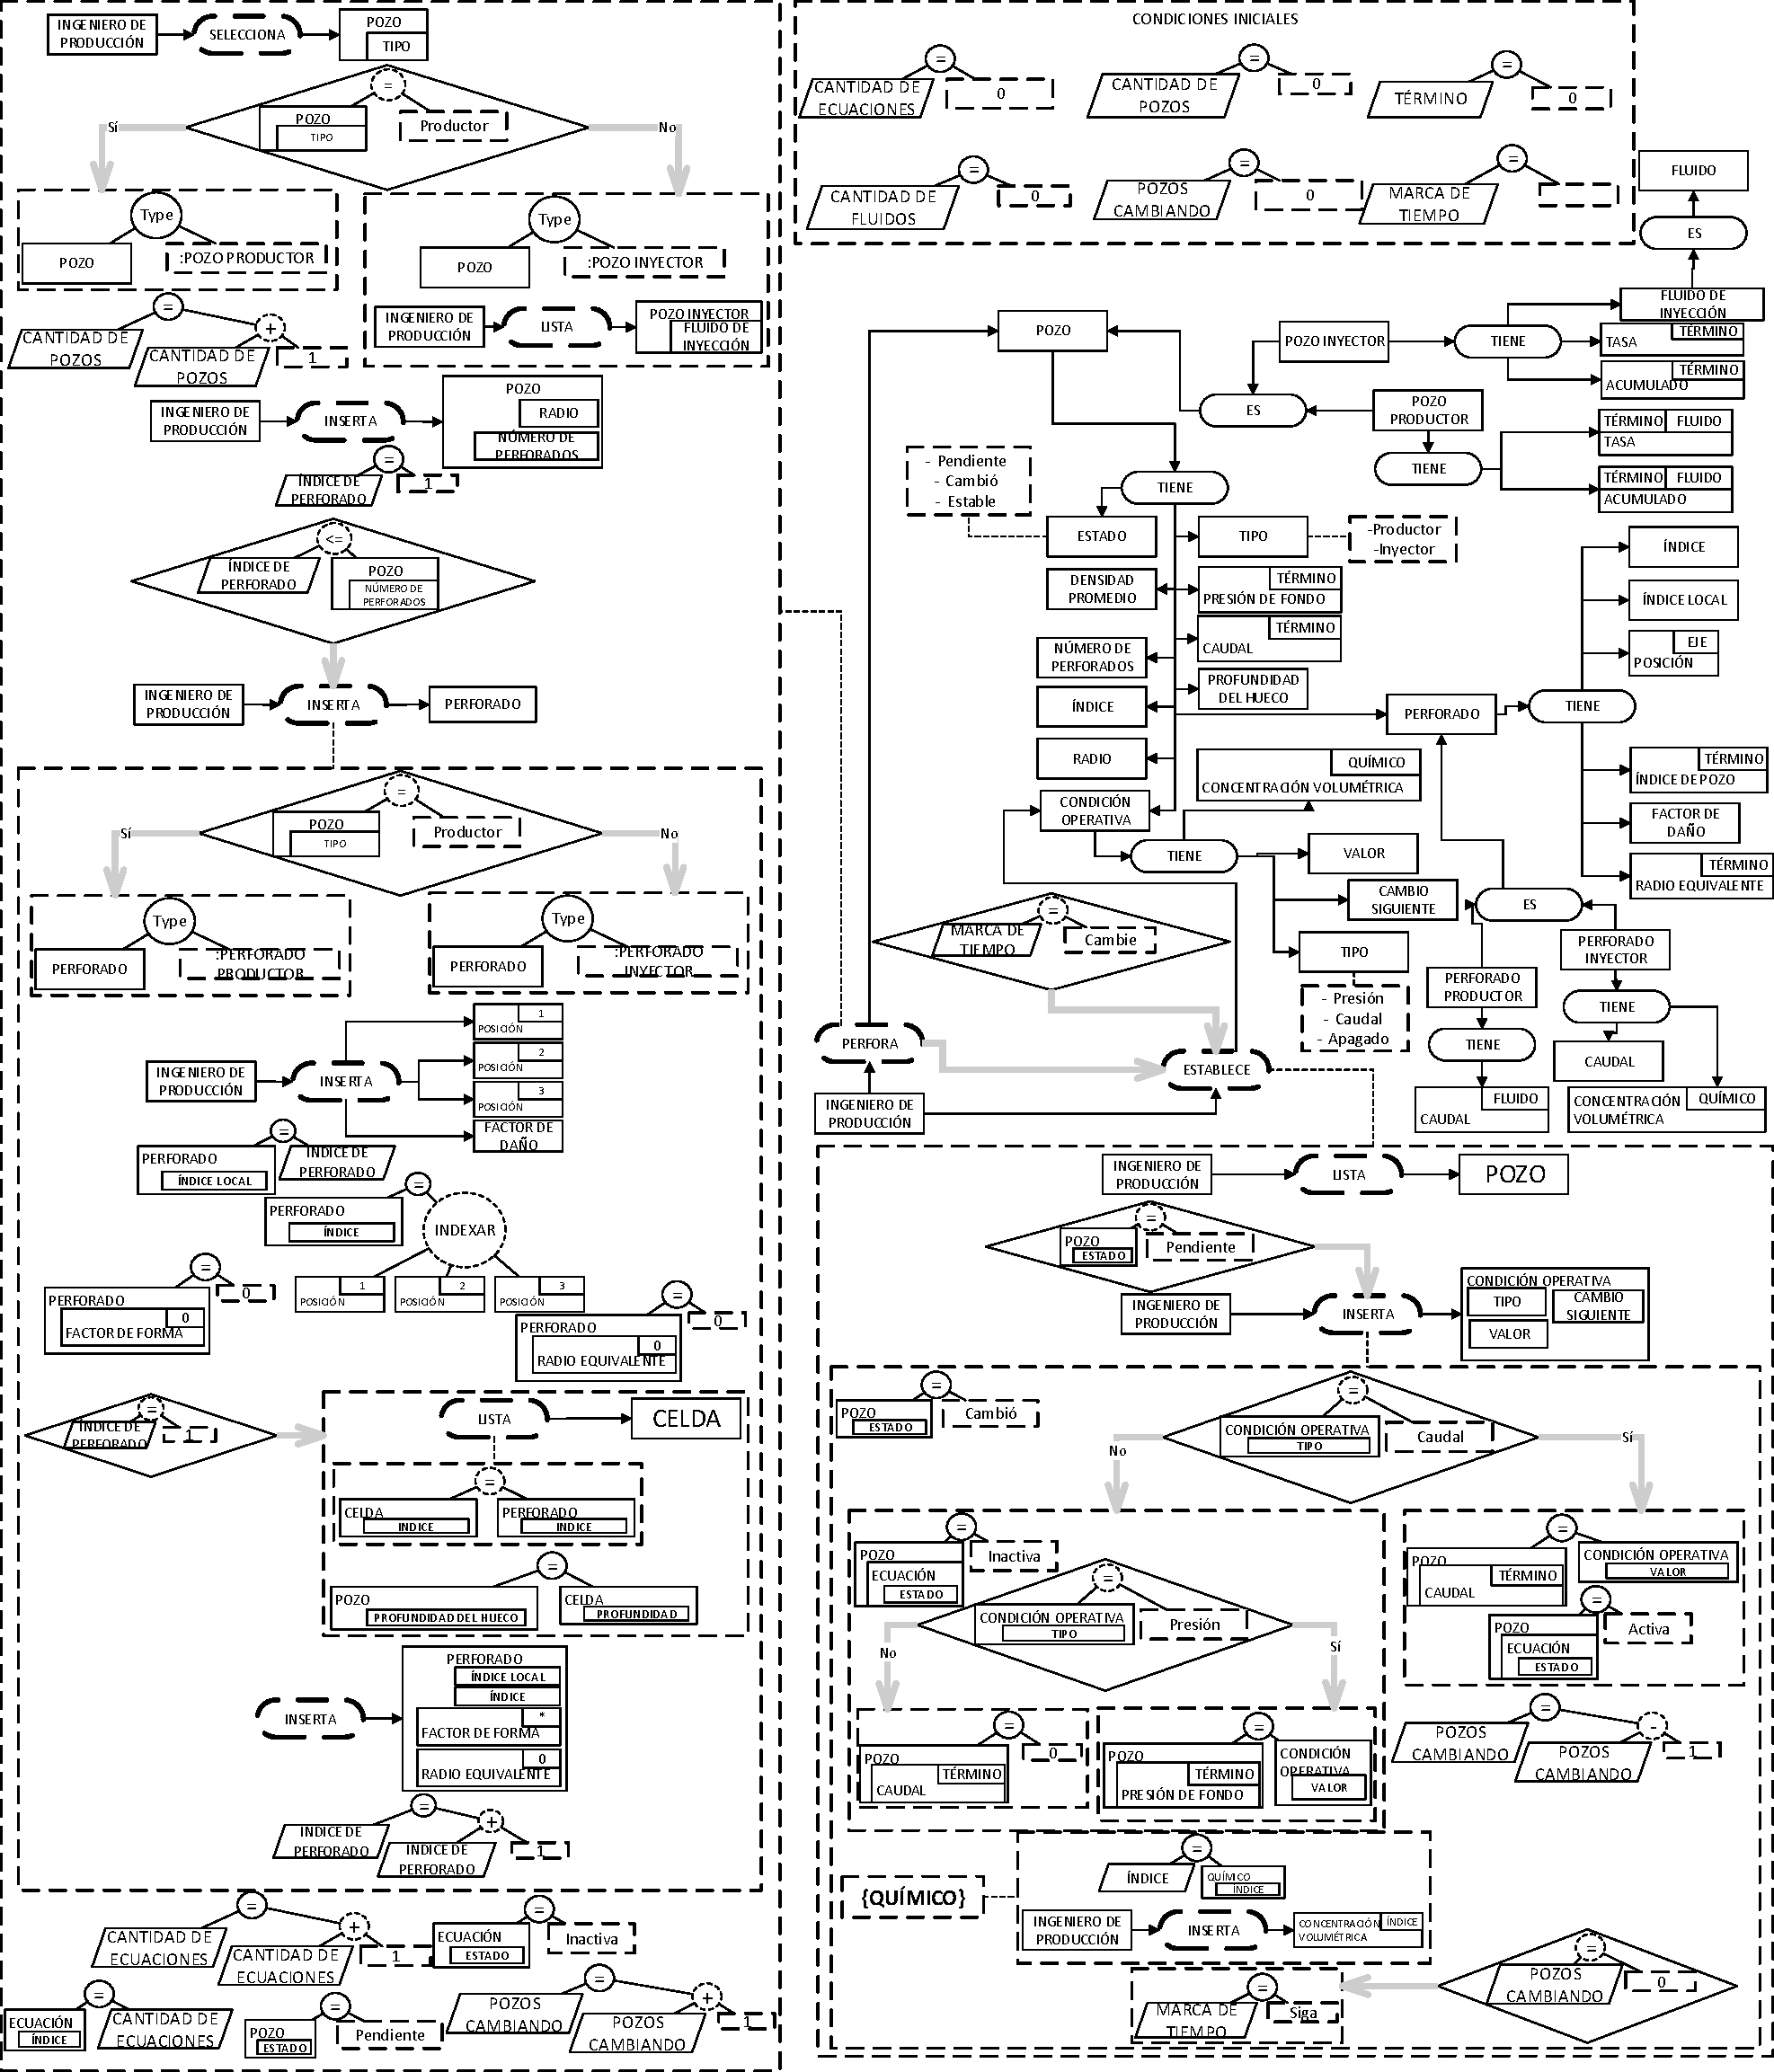
\includegraphics[width=0.9\linewidth]{Fig/Pozo.pdf}%
	\caption[Perforación de Pozos.]{Perforación de Pozos. Los autores.} \label{fig:Well}
\end{figure}

La principal diferencia entre los pozos productores e inyectores radica en que el pozo inyector tiene un ``fluido de inyección''. Además, la ``tasa'' y el ``acumulado'' del pozo inyector sólo dependen de este fluido, mientras que para el pozo productor dependerá de la cantidad de fluidos caracterizados. Estos pozos están sujetos a la restricción de no cambiar su tipo, además para un pozo productor, su conjunto de perforados corresponderá también a perforados productores. Así, para los pozos inyectores serán perforados inyectores.\\

Los pozos funcionan bajo una ``condición operativa'', que permite regular la presión o el caudal al que estos inyectan o producen fluido. Estas condiciones definen, si un pozo genera una ecuación, o si su caudal se puede resolver directamente usando la presión de fondo. Por otro lado, las condiciones operativas pueden variar en el tiempo. Por esto, se requiere calcular o resolver el atributo que no está sujeto a la condición operativa cada que se establezca un cambio en la condición.

\subsection{Químico}\label{subsec:PS_Chemical}
El ``químico'' como concepto comprende un conjunto de ``transferencias'' en las que se describen las cinéticas en no-equilibrio entre dos fluidos que pueden acarrear tal químico\footnote{Todas las transferencias del químico, en esta Tesis de Maestría, se consideran en no-equilibrio.}. Una transferencia es unidireccional\footnote{En el caso de las cinéticas reversibles o bidireccionales, se consideran dos transferencias.}, por lo que existe una cantidad de químico (``cantidad transferida'') que se transfiere de un ``fluido de origen'' a un ``fluido de destino'' y la ``cantidad transferida'' se calcula por medio de una ``función''.\\

La ``presencia'' de un químico en un fluido que lo acarrea, implica que se genere una ``afectación'' de las propiedades de tal ``fluido de acarreo''. Esta afectación se aplica por medio de una ``función'' en la que se calcula una ``modificación'', la modificación corresponde a una corrección que se aplica sobre el cálculo de la propiedad que se afecta. Con esta representación del químico es posible considerar múltiples productos químicos con los que se generan afectaciones en diferentes fluidos, pudiendo ser tanto de incremento como reducción, a la viscosidad de los mismos o a su permeabilidad relativa. En la Figura \ref{fig:Chemical} se presenta la representación del químico.\\

\begin{figure}[h]
	\centering%
	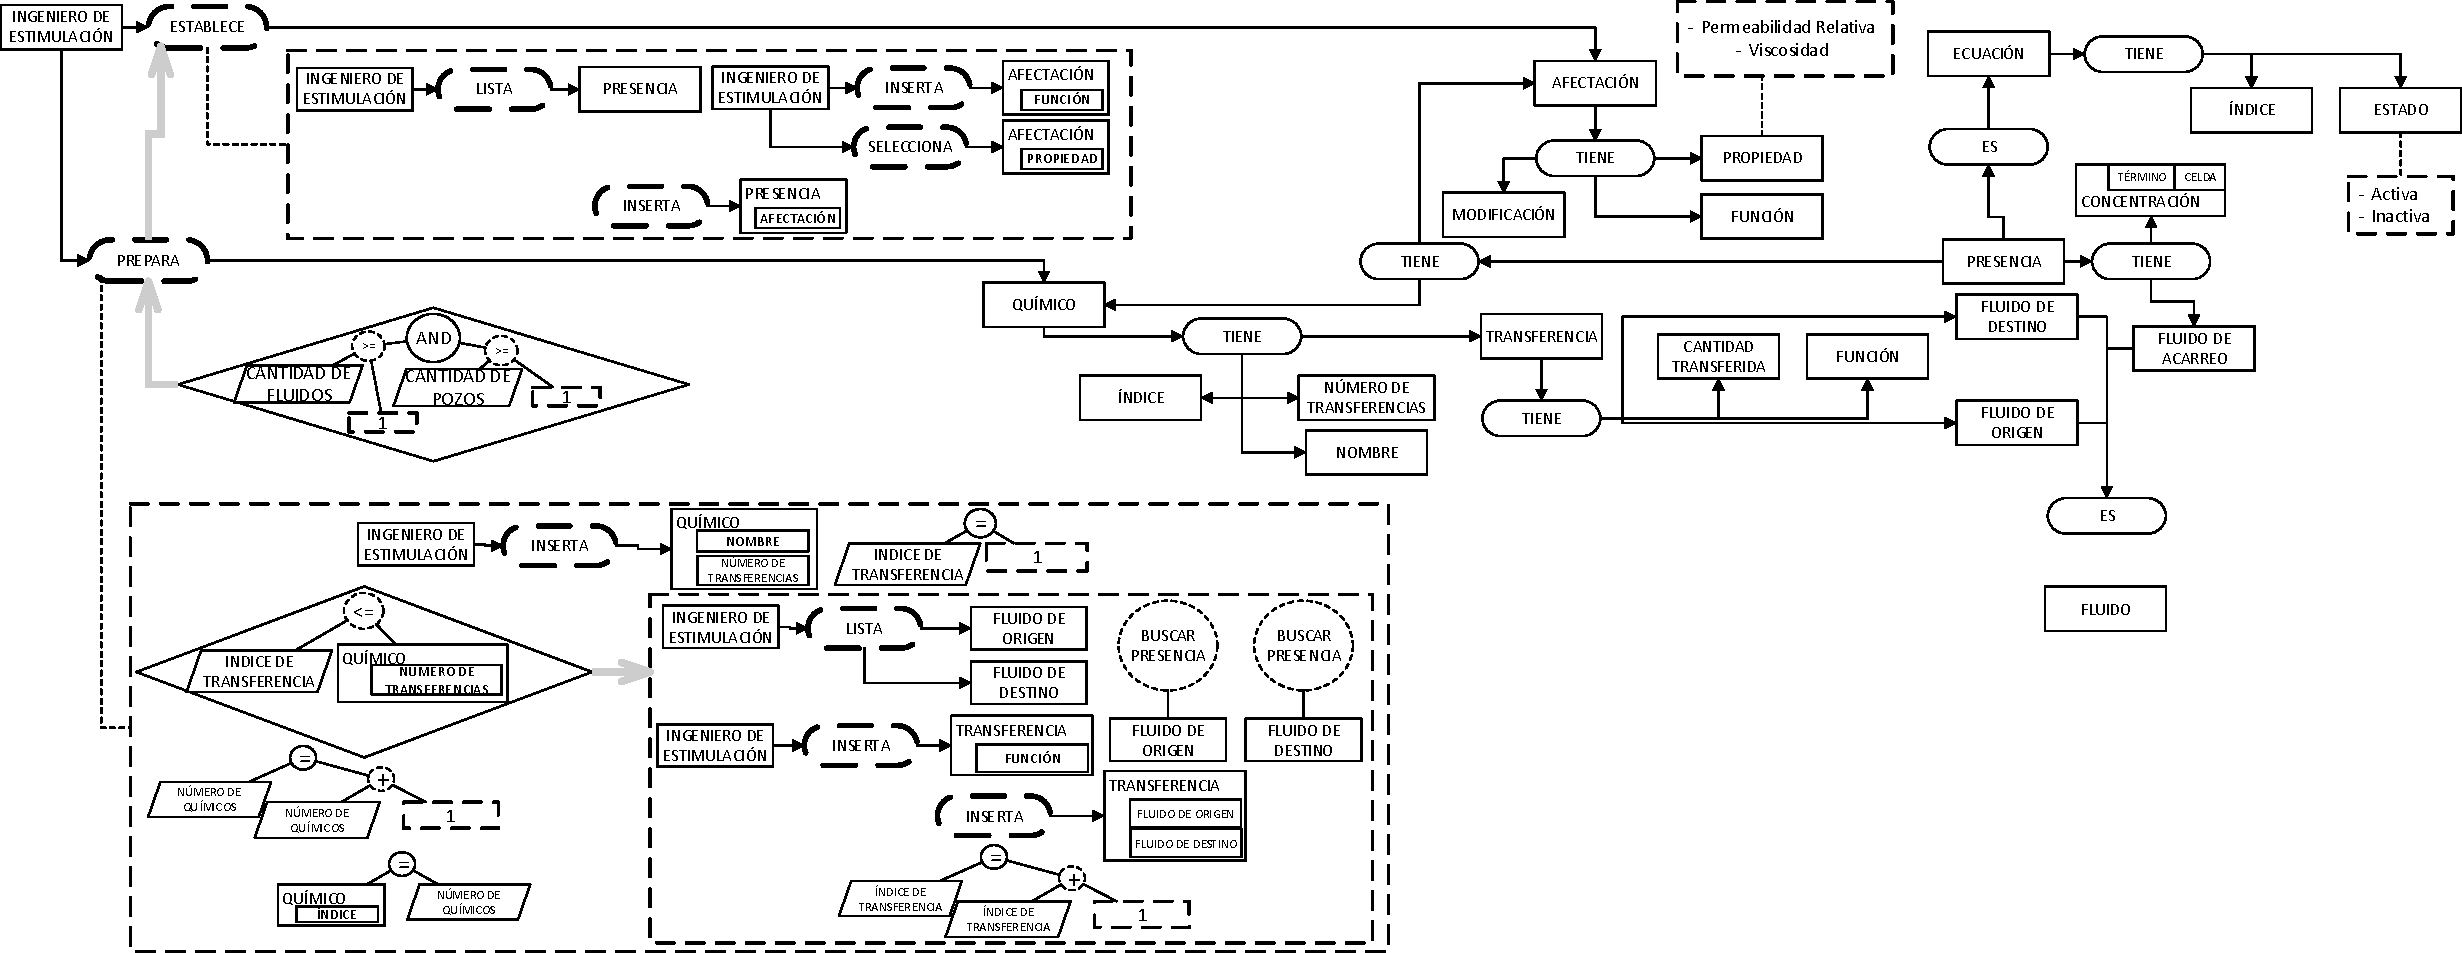
\includegraphics[width=0.9\linewidth]{Fig/QuimicoStruct.pdf}%
	\caption[Preparación del Químico.]{Preparación del Químico. Los autores.} \label{fig:Chemical}
\end{figure}

En la relación dinámica ``Ingeniero de estimulación prepara químico'' el ``Ingeniero de estimulación'' caracteriza todas las transferencias que puede tener el químico, indicando en cada una la expresión matemática, en la que se describe la ``función'' a evaluar, para calcular la ``cantidad transferida''. Así mismo, caracteriza las afectaciones que se generan, considerando que no todas las presencias del químico pueden verse afectadas por el mismo, y de manera análoga a la transferencia, indica la expresión matemática o ``función'' para calcular la ``modificación''. Posteriormente, el ``Ingeniero de estimulación'' indica unas condiciones iniciales del químico en el yacimiento, es decir, para todas las celdas de la malla al tiempo inicial o tiempo cero. 

\subsection{Ecuación}\label{subsec:PS_Equation}
La ecuación es un concepto abstracto que sirve como agrupador. Tanto el fluido, como el pozo, o presencia de un químico en un fluido\footnote{Esto debido a que todas las transferencias o cinéticas se consideran en no-equilibrio.}, son ecuaciones. Este concepto sirve para iterar sobre todos los conceptos que generan un residual en el método de Newton. Tienen un índice y estado. Este último permite activar o desactivar la solución de ecuaciones, lo cual sirve para gestionar la solución de pozos involucrando cambios de condición operativa.
%Poner ecuación acá con Volumen de celda ya como concepto


%\section{PS Representation of Enhanced Oil Recovery Simulation}\label{sec:PS_EOR}
\section{Funciones y eventos para la simulación de procesos EOR}\label{subsec:PS_EOR}
En el esquema \ref{fig:PSComplete} se evidencia la solución del BOM discretizado usando volúmenes finitos en una malla cartesiana ortogonal. El paso a paso en la ejecución de los eventos se muestra en \ref{fig:EventsInteraction}.  En el evento ``Presión del fluido varía'' se desarrollan las iteraciones del método de Newton-Raphson e internamente las iteraciones sobre las celdas requeridas para solucionar el sistema algebraico resultante de la discretización. En las secciones siguientes se explica el EP elaborado en las respectivas porciones correspondientes a eventos, subrutinas y funciones que procesan la simulación de procesos EOR. Para el correcto desarrollo de la simulación, se establecen las siguientes \textbf{precondiciones}: existe una única malla y una única roca. En el caso de una simulación de dos fluidos debe existir una única interacción entre fluidos. En el caso de tres fluidos deben existir exactamente dos interacciones entre fluidos.



%In this section we propose a PS representation for enhanced oil recovery simulation, we couple a black oil model discretized using finite volumes method with the theoretical framework developed the previous chapter. We mapped each term in the resultant equations to their respective concepts and how they are linked together. The complete representation is shown in \ref{fig:PSComplete}.\\
\begin{figure}[h]
\centering%
\includegraphics[width=1\linewidth]{Fig/EPConQuimico.pdf}%
%\caption{Complete PS Representation for EOR Processes} \label{fig:PSComplete}
\caption[Representación en EP de la simulación de procesos EOR.]{Representación en EP de la simulación de procesos EOR. Los autores.} \label{fig:PSComplete}
\end{figure}

\begin{figure}[h]
	\centering%
	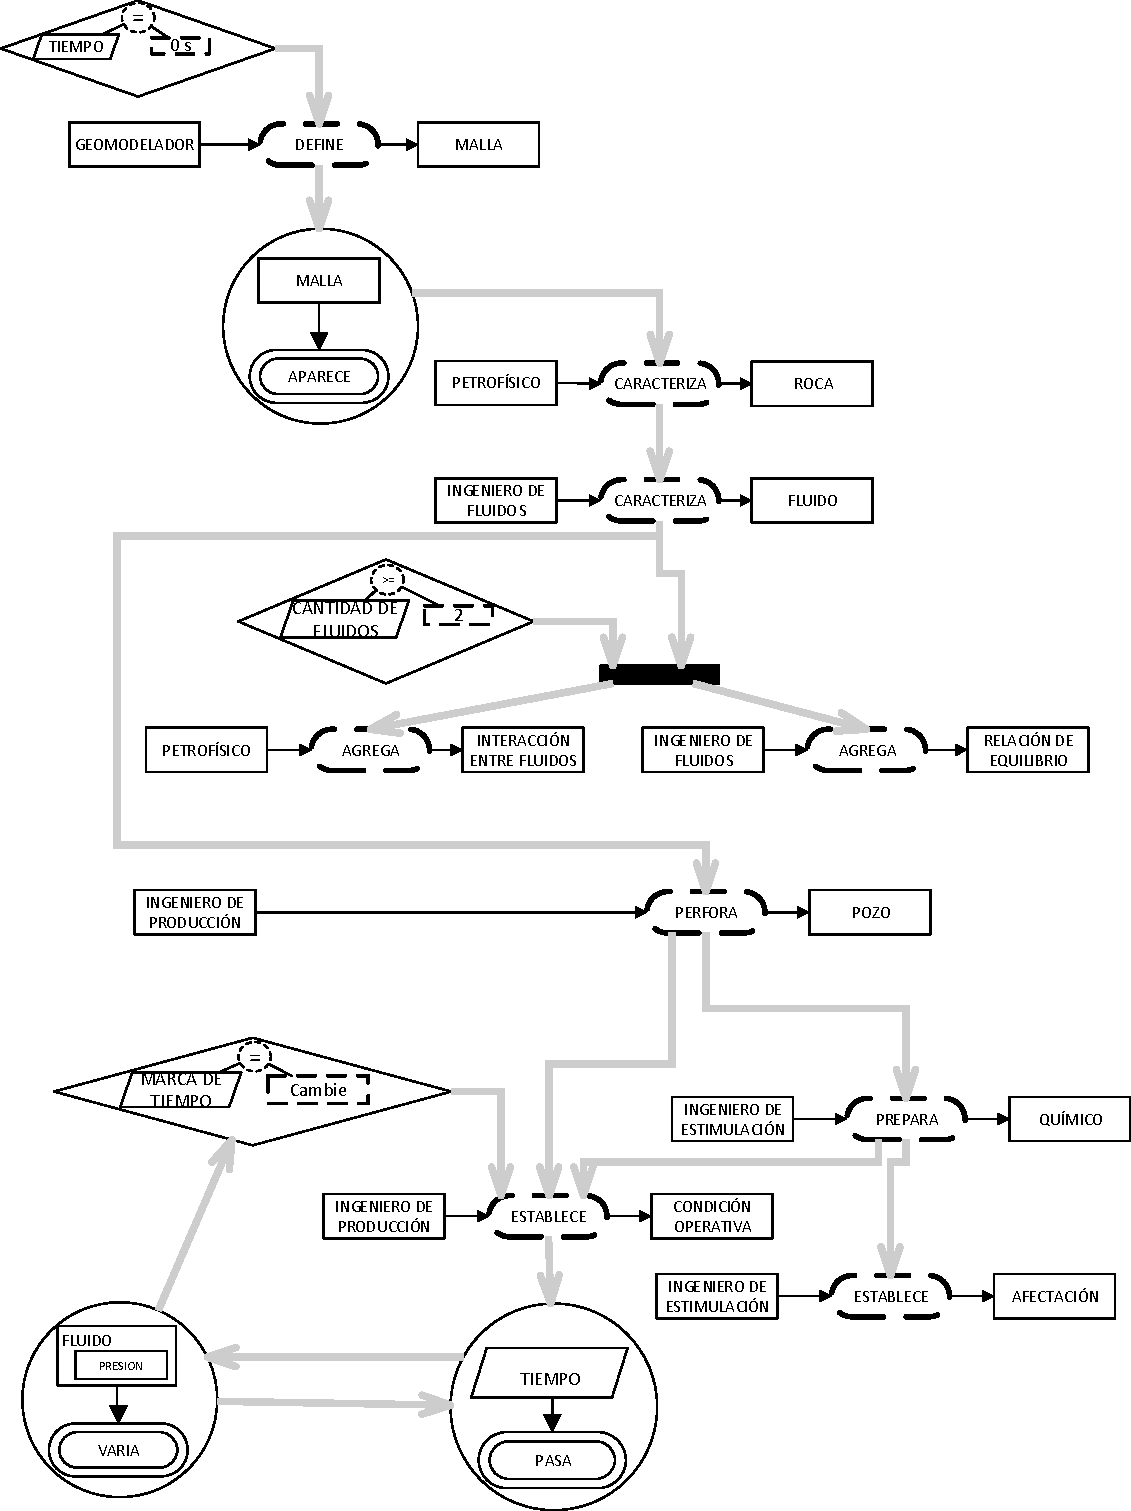
\includegraphics[width=0.9\linewidth]{Fig/FlujoDeEventos.pdf}%
	%\caption{Complete PS Representation for EOR Processes} \label{fig:PSComplete}
	\caption[Diagrama basado en el grafo de interacción de eventos.]{Diagrama basado en el grafo de interacción de eventos. Los autores basados en \cite{zapata2013Eventos}.} \label{fig:EventsInteraction}
\end{figure}
%The rest of this section is as follows: In section \ref{sec:PS_Mesh} we present the Mesh concept as a collection of cells with additional elements needed for calculating the attributes of each cell. Furthermore, we develop the dynamical relationship ``Geomodeler defines Mesh'' as an interaction of the role ``Geomodeler'' with atomic\footnote{atomic as is stated by \cite{AG01} (Aca debe ir Zapata)} dynamical relationships. In section \ref{sec:PS_Rock} we present the Rock concept with its attributes and initial characterization. In section \ref{sec:PS_Phase} ... In section \ref{sec:PS_Interphase} ... In section \ref{sec:PS_Equilibrium} we define the partition coefficients as relations between two phases, one contributing mass and another receiving mass in the mass balance equation. In section \ref{sec:PS_Well}

\subsection{Cálculo de propiedades}\label{subsec:PS_PropertyCalc}
En la subrutina ``Calcular propiedades'' se engloba el cálculo de propiedades que dependen de las incógnitas principales de la simulación (véase \ref{subsec:BOM}, ecuaciones constitutivas). En esta subrutina se itera sobre todos los fluidos y, para el fluido principal, calcula su saturación y su permeabilidad relativa (véase \ref{subsec:PS_Interphase}), en función de la saturación de los fluidos no principales. Además, para los fluidos no principales, calcula su presión con base en la presión del fluido principal y la presión capilar a la saturación del fluido de referencia. Una vez se tienen las presiones de todos los fluidos en el sistema, es posible interpolar sus factores volumétricos y viscosidad en términos de su presión. Adicionalmente, se calculan sus densidades, usando la formulación que se propone en la Ecuación \ref{ec:generaldensity}, para todas las relaciones de equilibrio existentes.  En la Figura \ref{fig:PropertyCalculation} se muestra la representación de la subrutina ``Calcular Propiedades''.\\

\begin{figure}[h]
	\centering%
	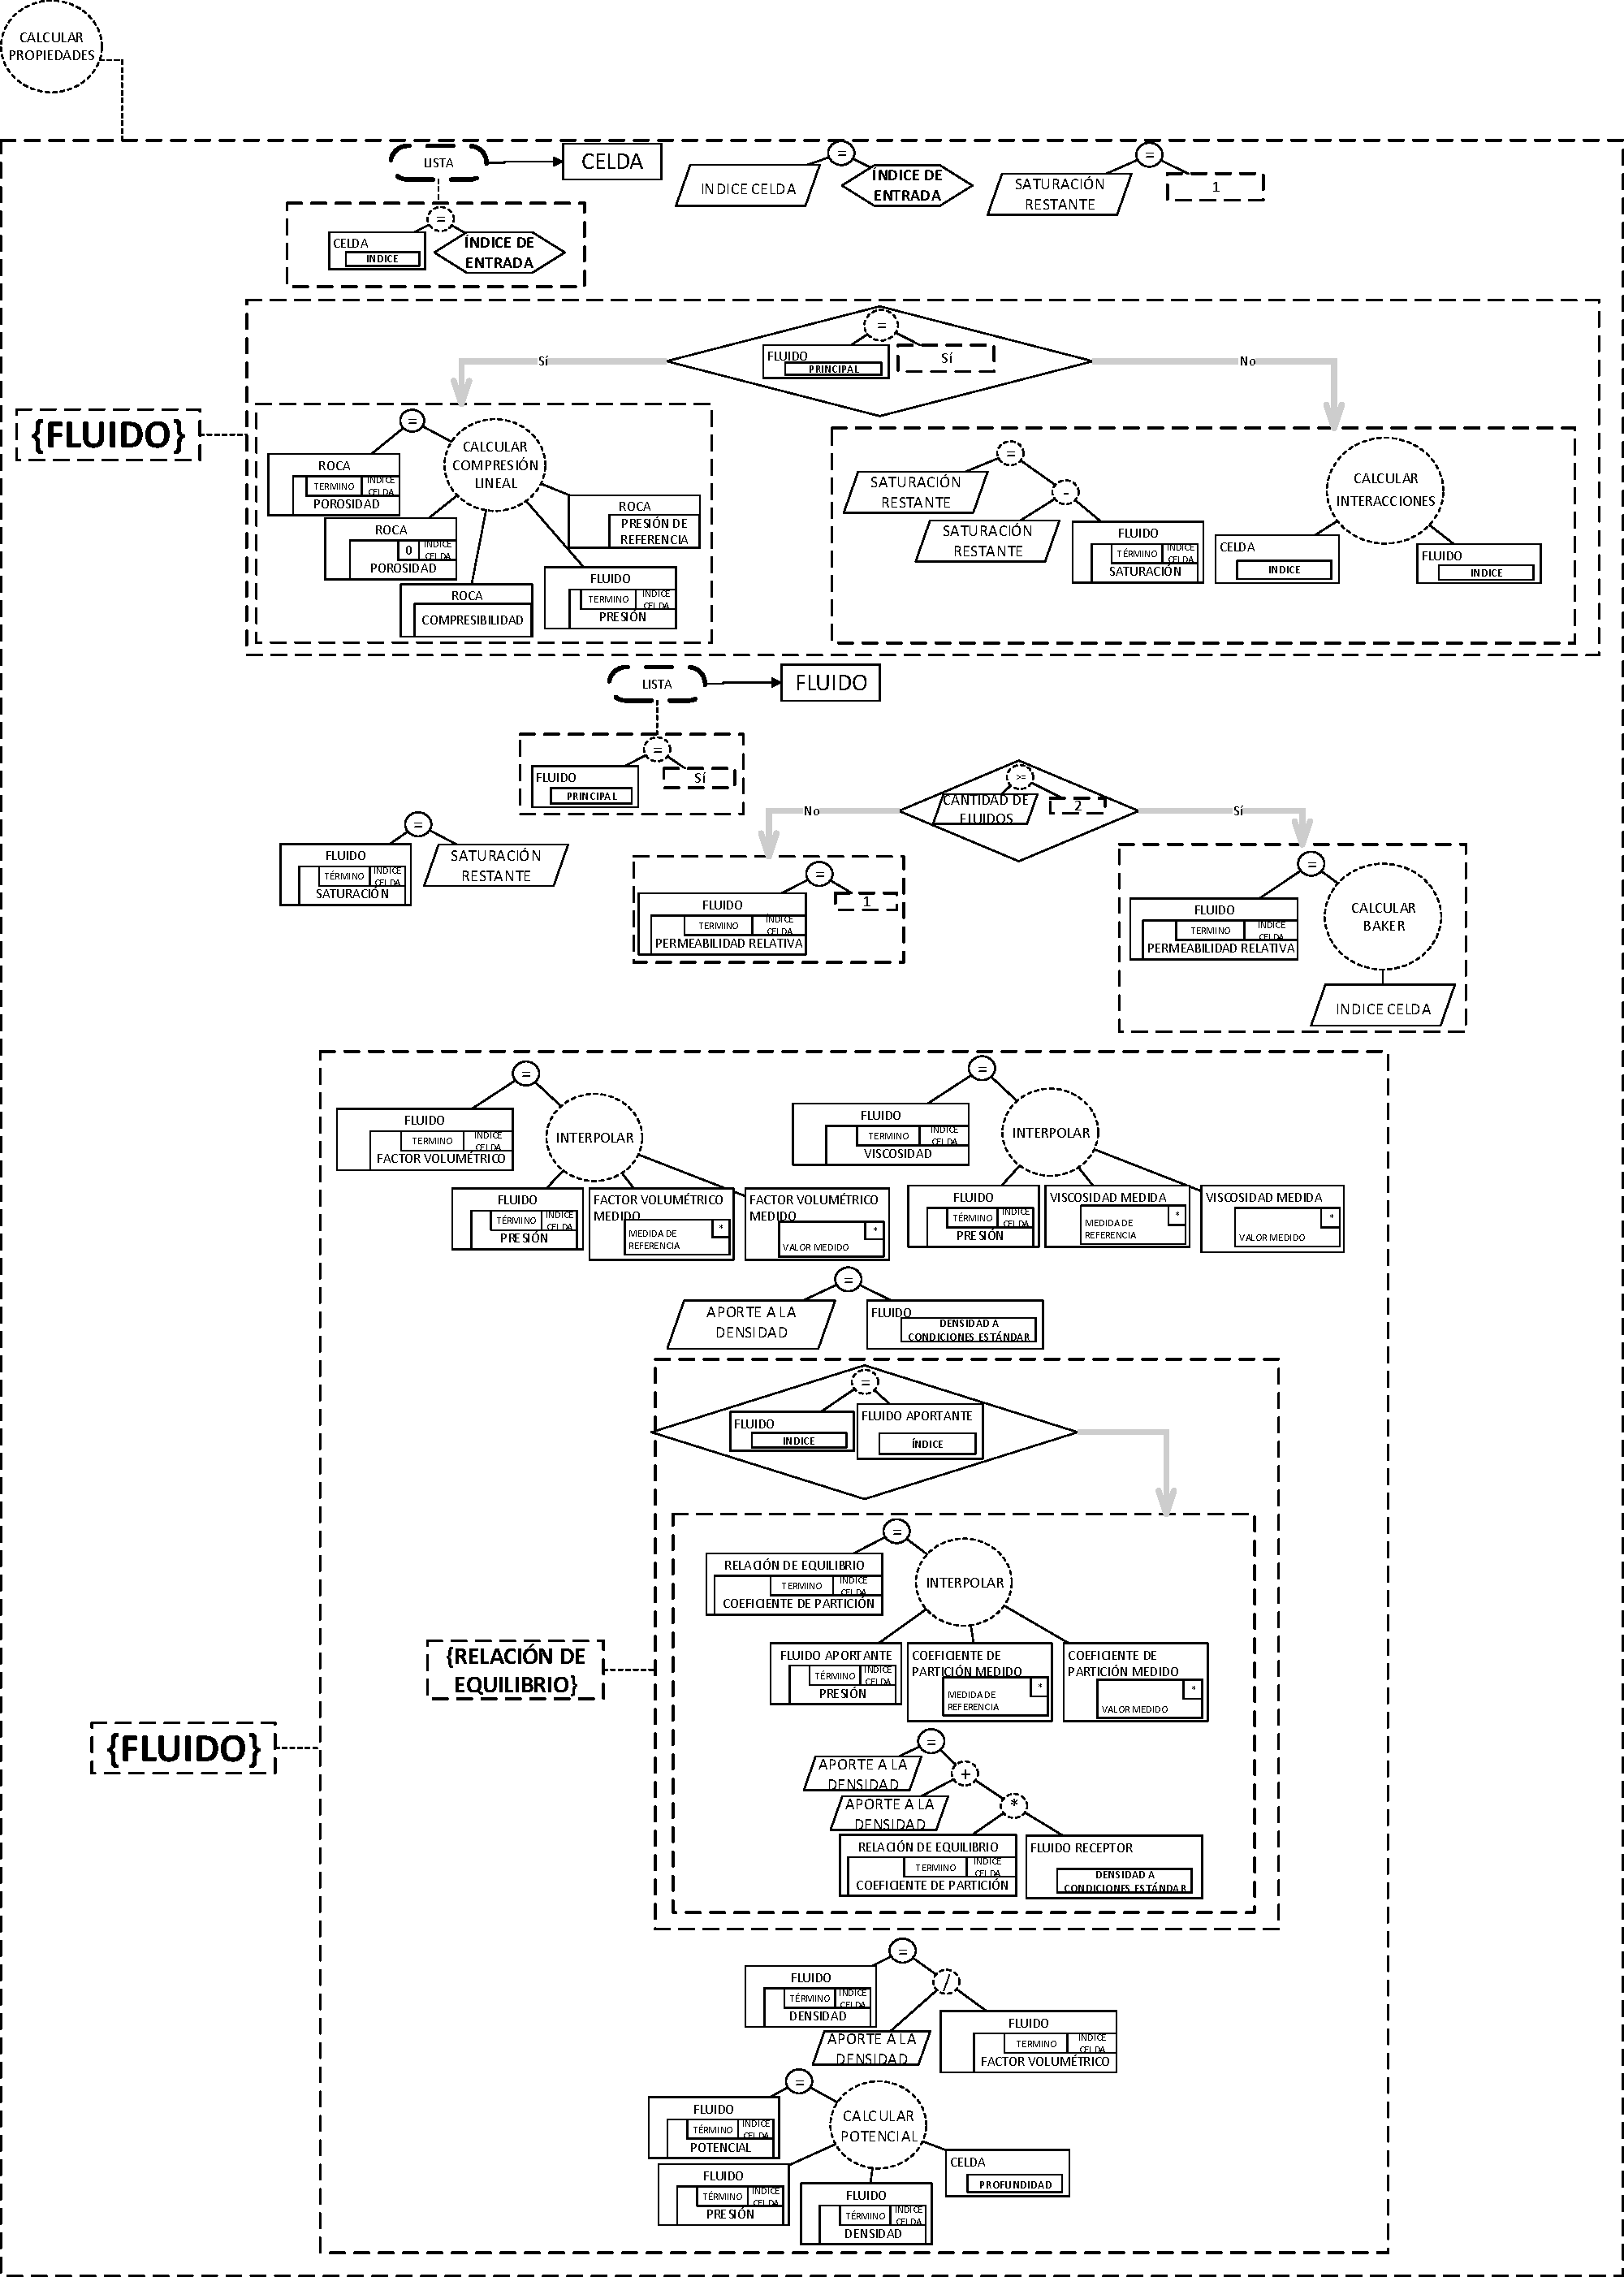
\includegraphics[width=0.9\linewidth]{Fig/CalculoPropiedades.pdf}%
	%\caption{Complete PS Representation for EOR Processes} \label{fig:PSComplete}
	\caption[Subrutina ``Calcular propiedades''.]{Subrutina ``Calcular propiedades''. Los autores.}
	\label{fig:PropertyCalculation}
\end{figure}

En la Figura \ref{fig:CapillaryPressure} se muestra la representación de la subrutina ``Calcular interacciones'' para el cálculo de presiones de los fluidos que no son principales. En esta subrutina se calculan las presiones capilares a la saturación del respectivo fluido de referencia, el cual corresponde a uno de los fluidos no principales, y con esta presión capilar, se calcula la presión del fluido, usando la Ecuación \ref{ec:presioncapilar}. Adicionalmente, se interpolan las permeabilidades relativas de los fluidos no principales, asumiendo que sólo dependen de su respectiva saturación.

\begin{figure}[h]
	\centering%
	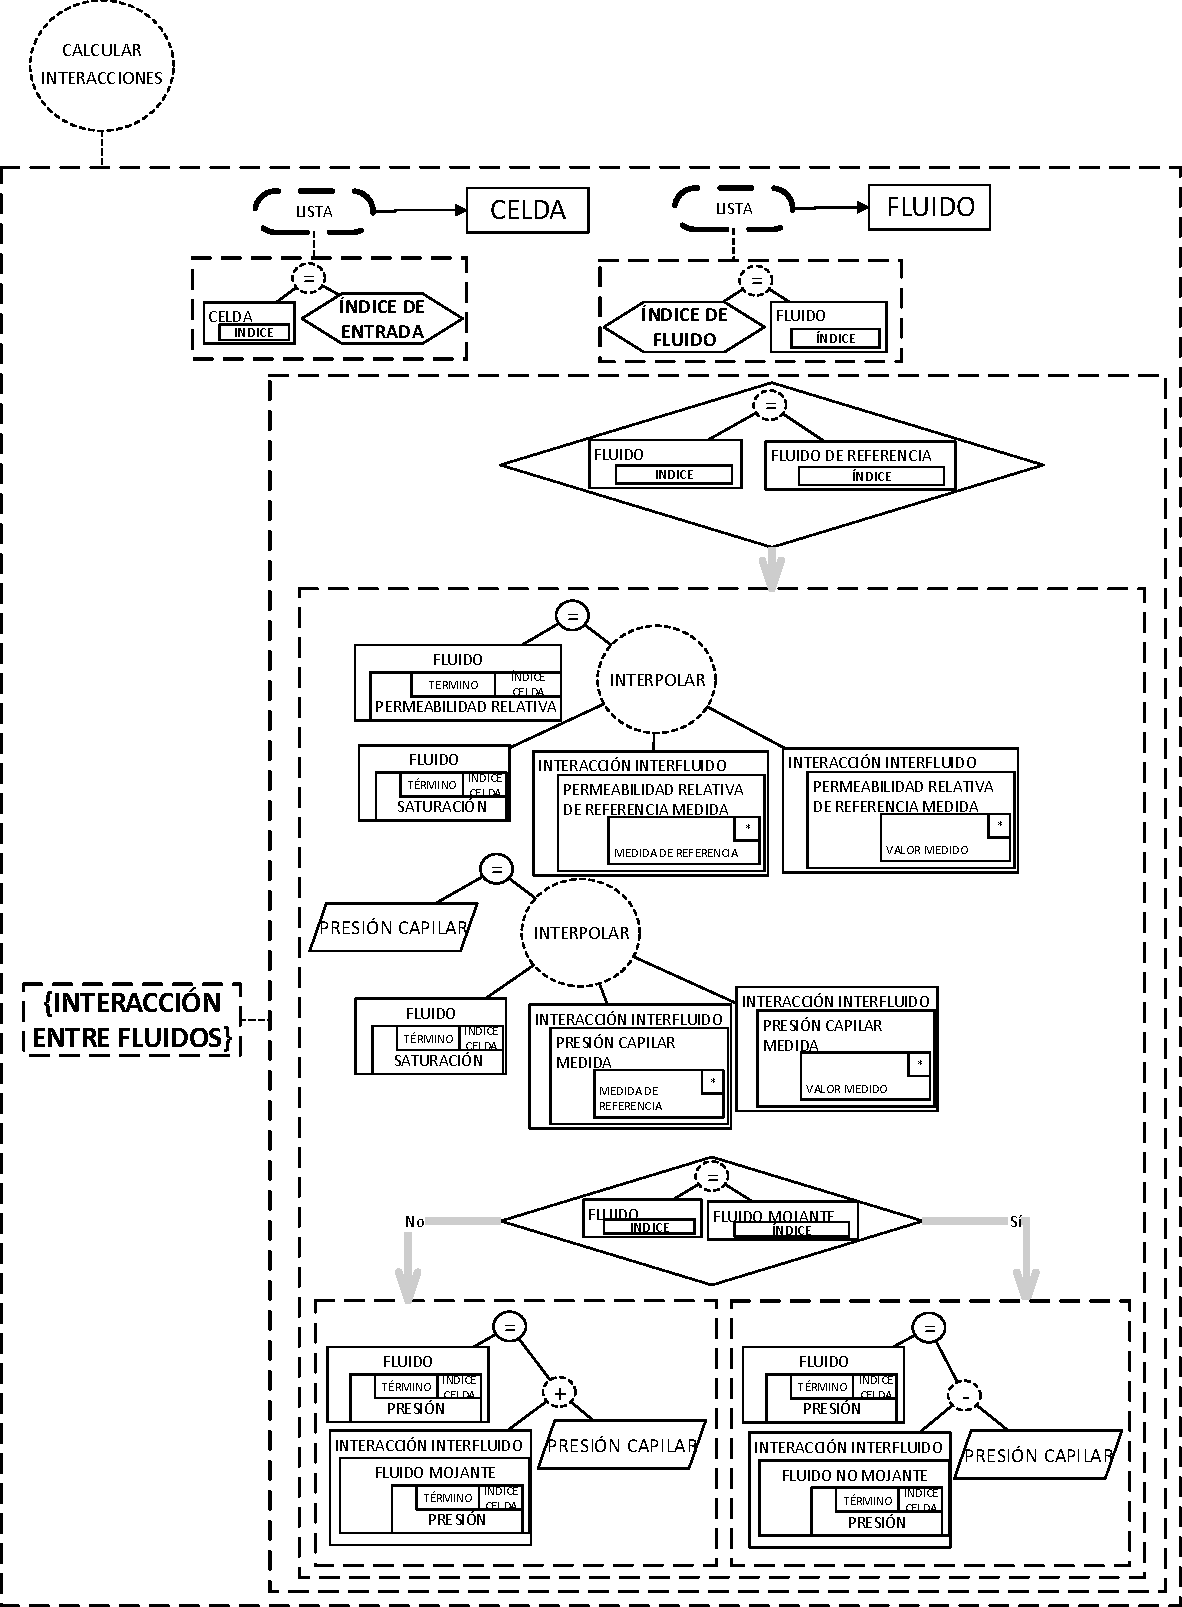
\includegraphics[width=0.9\linewidth]{Fig/CalcularInteracciones.pdf}%
	%\caption{Complete PS Representation for EOR Processes} \label{fig:PSComplete}
	\caption[Subrutina ``Calcular interacciones''.]{Subrutina ``Calcular interacciones''. Los autores.}
	\label{fig:CapillaryPressure}
\end{figure}

\subsection{Funciones y subrutinas de pozo}\label{subsec:PS_WellFunctions}
Los pozos tienen su ecuación sujeta a su condición operativa, requiriendo calcular el caudal en el pozo a una presión de fondo fija, o requiriendo estimar la presión de fondo para una condición de caudal fijo. Para esto se definen dos subrutinas: ``Estimar presión pozo'' y ``Calcular pozo''. En la primera, se despeja la presión de fondo del pozo, a partir de su respectiva ecuación de Peaceman \citep{peaceman1983interpretation}, usando la condición operativa de caudal fijo. En la segunda, se calcula la ecuación de \cite{peaceman1983interpretation} para todos los perforados, usando la presión de fondo fija, y se suman para así obtener el caudal. En la Figura \ref{fig:EstimatePwf} se presenta la subrutina ``Estimar presión pozo'' y en la Figura \ref{fig:CalculateFlow} se muestra la subrutina ``Calcular pozo''. Cabe notar que la subrutina ``Calcular pozo'' depende de la subrutina ``Calcular perforado'' y ``Calcular perforado'' requiere, a su vez, de ``Calcular Peaceman Productor'' y ''Calcular Peaceman Inyector''. 

\begin{figure}[h]
	\centering%
	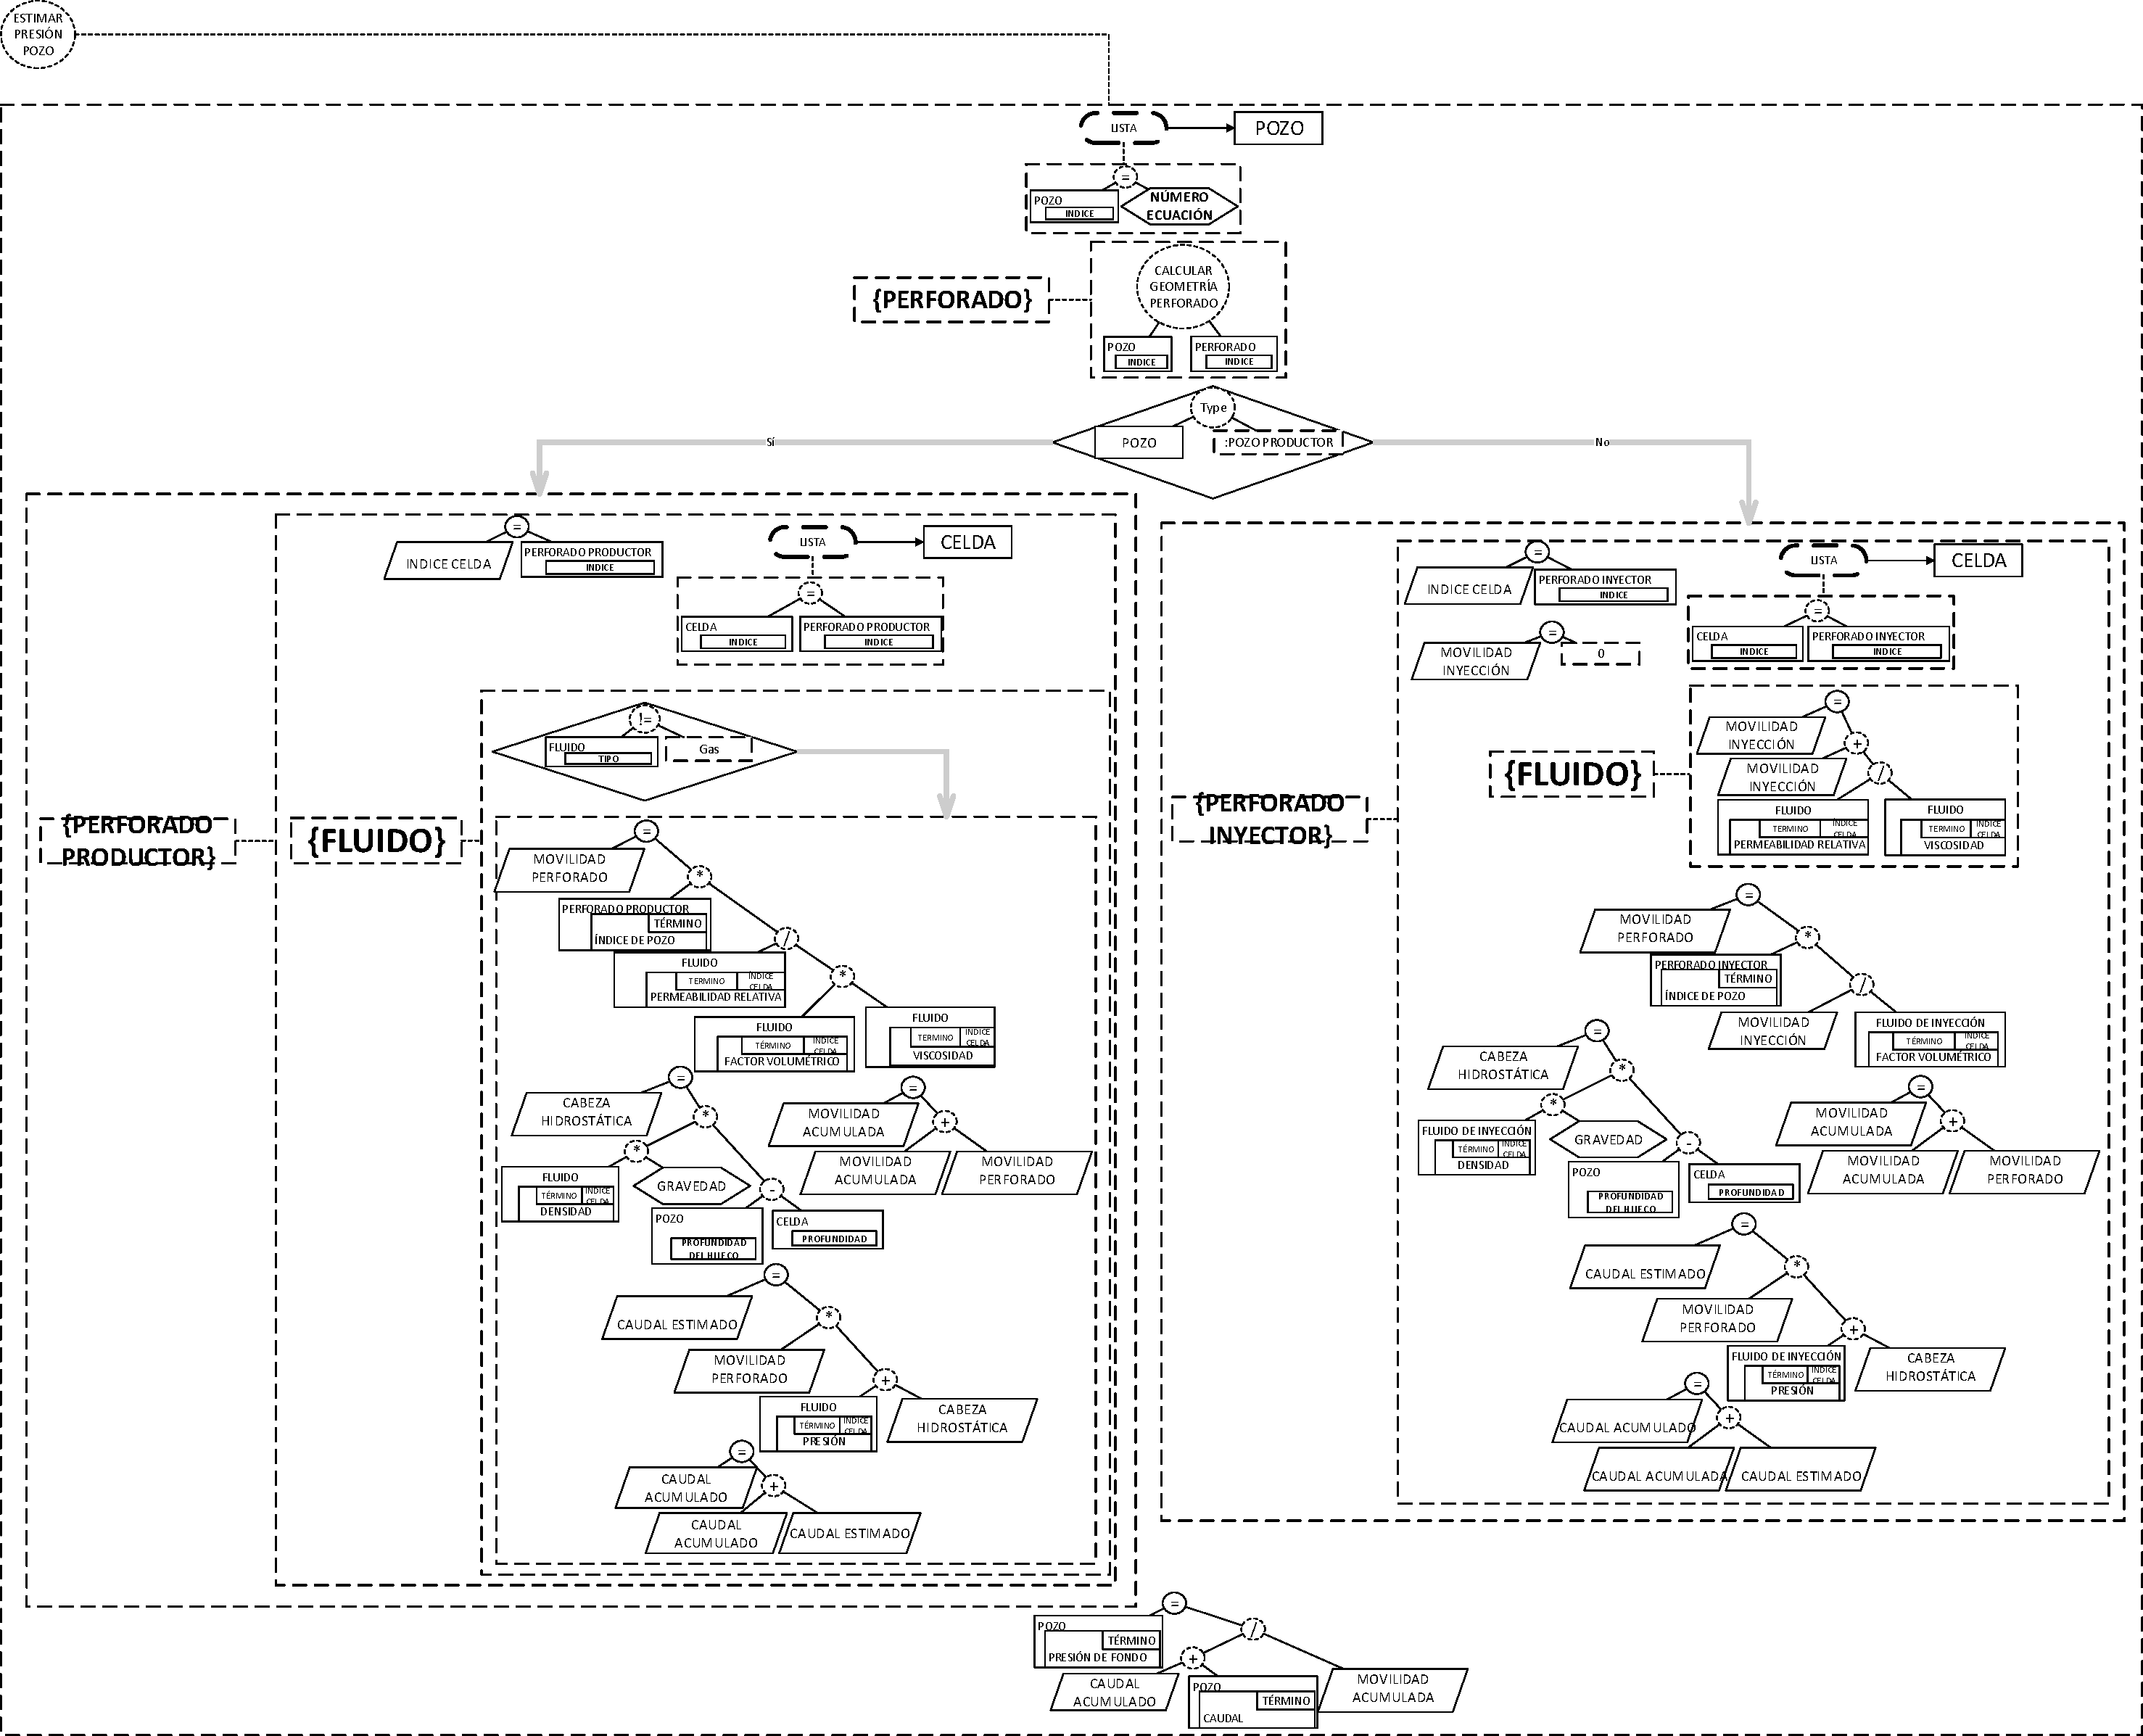
\includegraphics[width=1\linewidth]{Fig/EstimarPwf.pdf}%
	%\caption{Complete PS Representation for EOR Processes} \label{fig:PSComplete}
	\caption[Subrutina ``Estimar presión pozo''.]{Subrutina ``Estimar presión pozo''. Los autores.}
	\label{fig:EstimatePwf}
\end{figure}

\begin{figure}[h]
	\centering%
	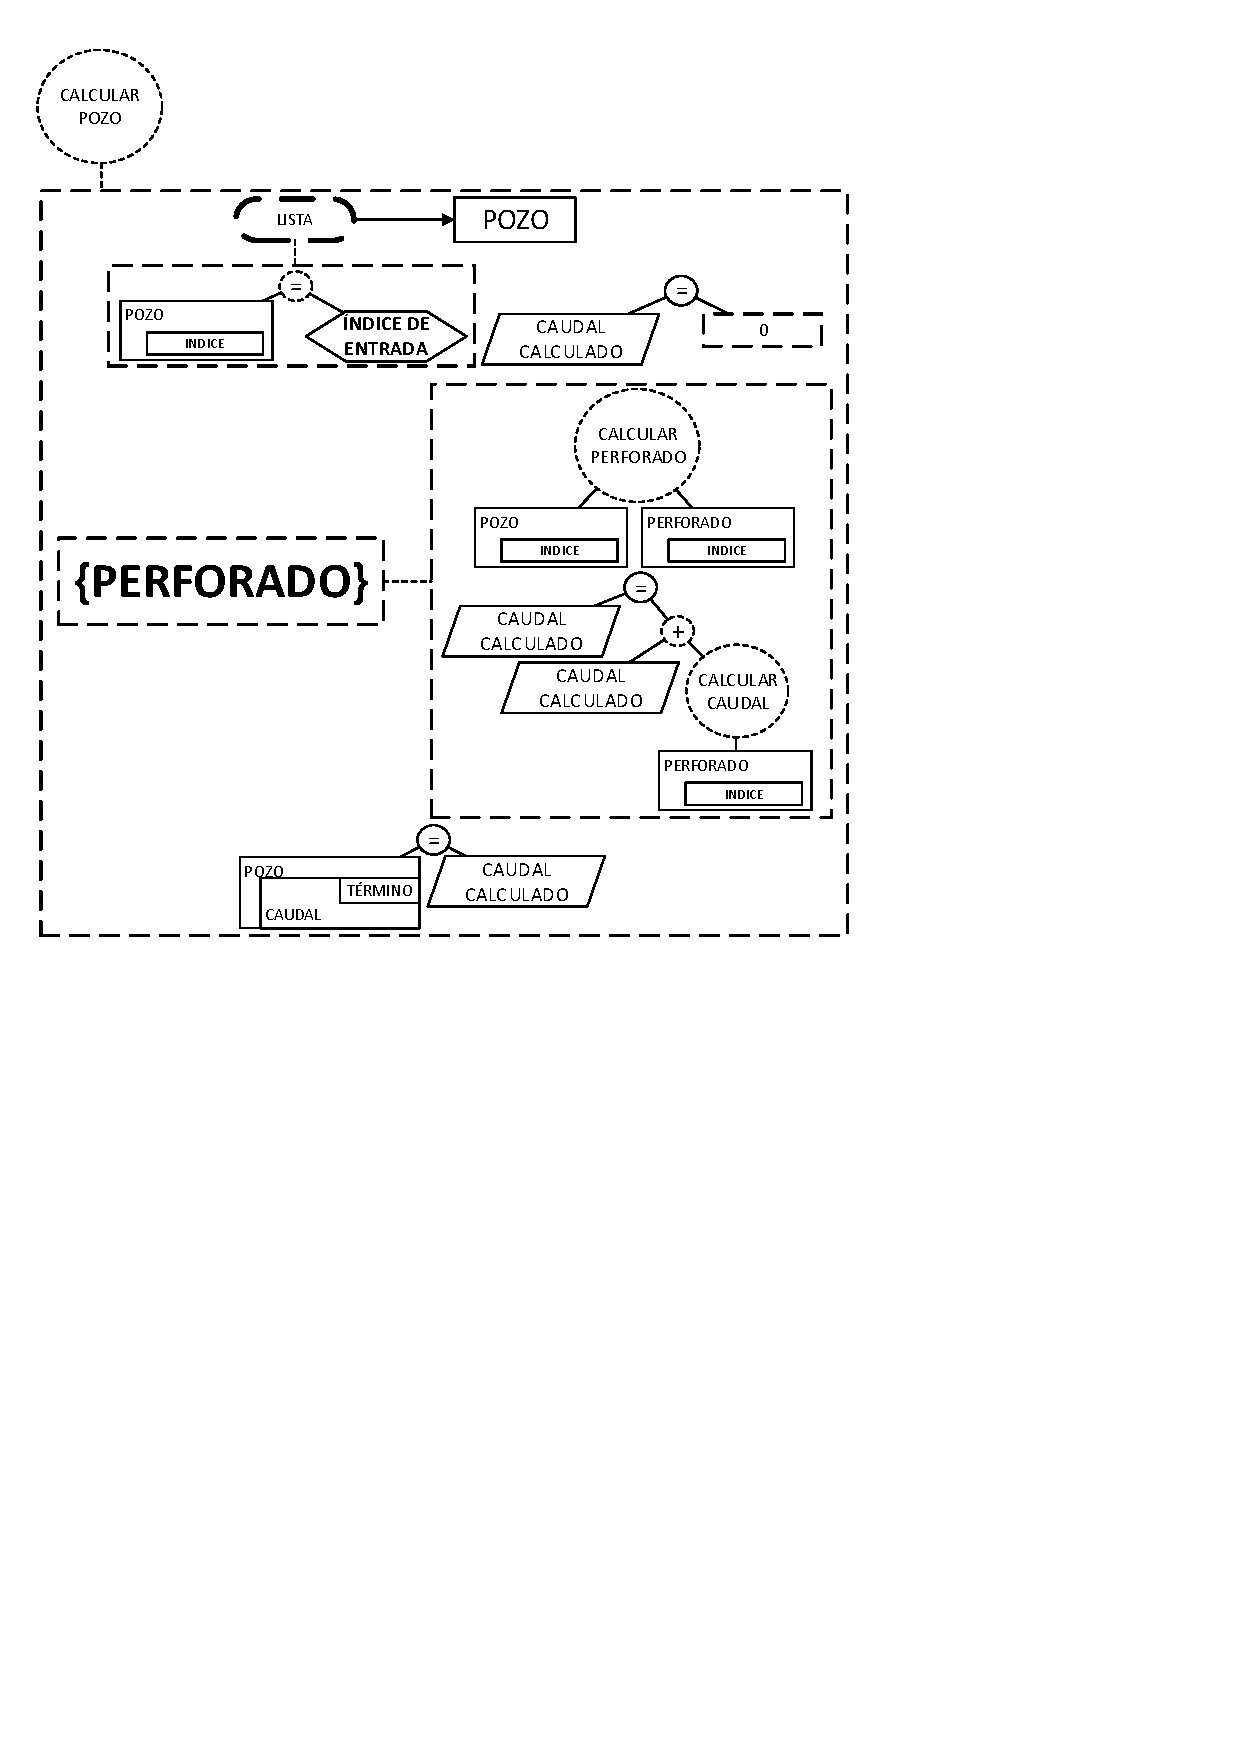
\includegraphics[width=1\linewidth]{Fig/CalcularPozo.pdf}%
	%\caption{Complete PS Representation for EOR Processes} \label{fig:PSComplete}
	\caption[Subrutina ``Calcular pozo''.]{Subrutina ``Calcular pozo''. Los autores.}
	\label{fig:CalculateFlow}
\end{figure}

\subsection{Tiempo pasa}\label{sec:PS_TimePasses}
El evento ``Tiempo pasa'' se dispara en el momento en que se tienen las suficientes realizaciones de los conceptos para ejecutar la simulación, es decir, se ejecutaron las mínimas relaciones dinámicas para poder disparar el evento, como se ve en la figura \ref{fig:TimePasses}. En este evento se procesa el inicio y el final de la simulación, incrementando el ``tiempo'' y ``término'' al que se van a calcular las propiedades de los conceptos principales.\\

Se puede observar también que, en este evento se realiza el cálculo de las propiedades iniciales para toda la malla. Debido a que, al término cero, sólo se tienen las propiedades que se insertan en las relaciones dinámicas ejecutadas previamente. las demás propiedades deben ser calculadas como se presenta en la figura \ref{fig:Concepts}, puesto que se requieren para el término de acumulación en las ecuaciones de transporte para todos los fluidos existentes.

\begin{figure}[h]
	\centering%
	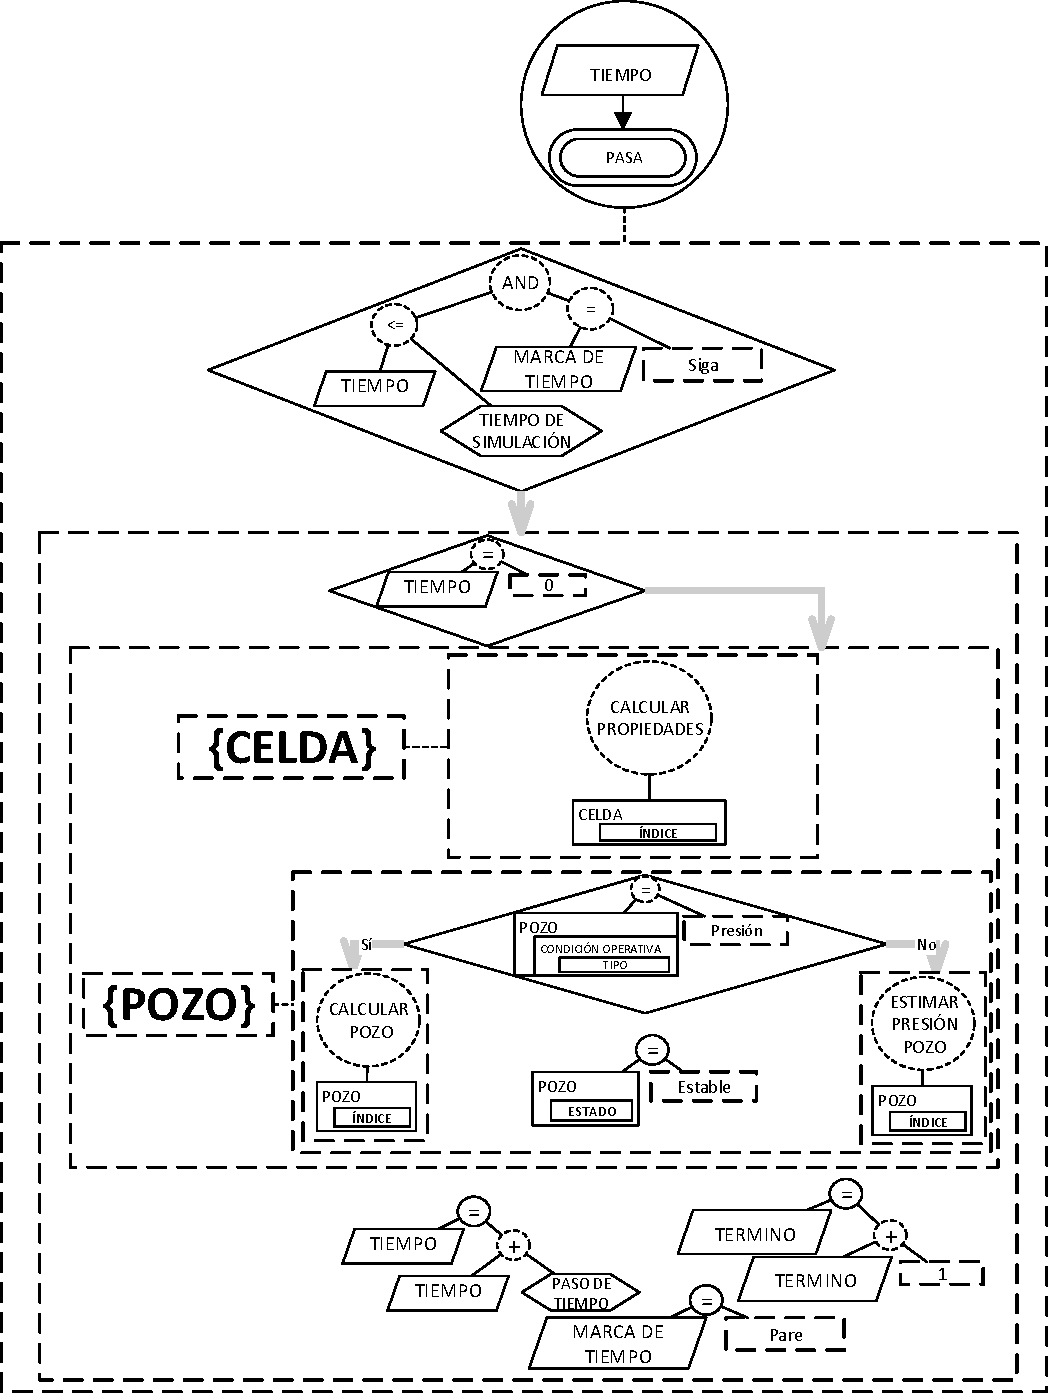
\includegraphics[width=0.7\linewidth]{Fig/TiempoPasa.pdf}%
	%\caption{Complete PS Representation for EOR Processes} \label{fig:PSComplete}
	\caption[Representación del paso del tiempo.]{Representación del paso del tiempo. Los autores.} \label{fig:TimePasses}
\end{figure}


\subsection{Presión del Fluido varía}\label{sec:PS_FluidVaries}
En el evento ``Presión del Fluido varía'' se procesa el núcleo de la simulación. En éste, se llevan a cabo las iteraciones del método de Newton-Raphson para converger al próximo paso de tiempo. La especificación de este evento consta de cinco procesos principales: La actualización de propiedades al término actual, el recálculo de las mismas, el cálculo de los residuales en cada iteración, el cálculo de la matriz jacobiana y la actualización de las incógnitas. Dentro de estos procesos principales se realizan, también, los correspondientes cálculos del transporte del químico. La especificación del evento ``Presión del Fluido varía'' se presenta en la figura \ref{fig:FluidPressureVaries}.\\

\begin{figure}[h]
	\centering%
	\includegraphics[width=0.9\linewidth]{Fig/PresionVaria.pdf}%
	%\caption{Complete PS Representation for EOR Processes} \label{fig:PSComplete}
	\caption[Especificación del evento Presión del fluido varía.]{Especificación del evento Presión del fluido varía. Los autores.} \label{fig:FluidPressureVaries}
\end{figure}

\subsubsection{Actualización de arreglos de propiedades}\label{subsec:PS_DefVars}
En la actualización de propiedades al término actual, se hace un incremento de tamaño y asignación del estimado inicial para el método de Newton-Raphson para todas las celdas de la malla, fluidos y propiedades dependientes del tiempo. Lo mismo sucede para los pozos y cada uno de sus perforados. La actualización de propiedades se expone en la figura \ref{fig:UpdateProperties}. 

\begin{figure}[h]
	\centering%
	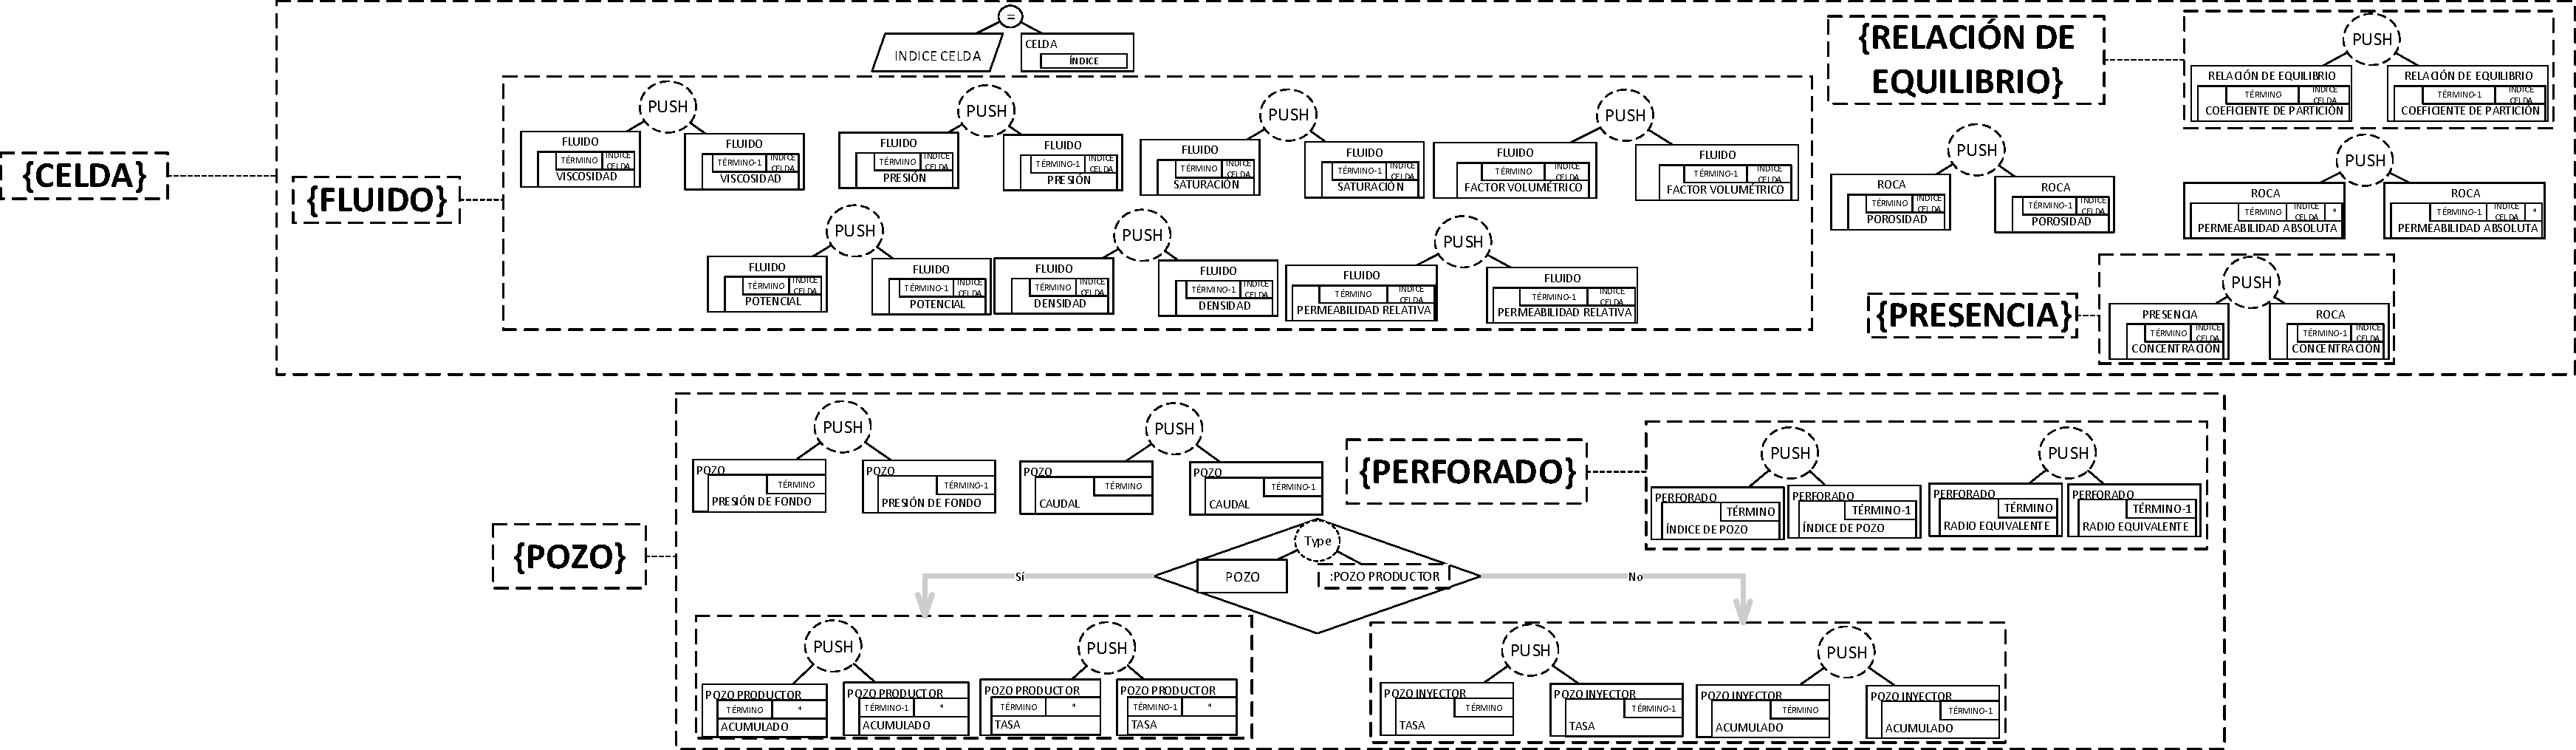
\includegraphics[width=\linewidth]{Fig/ActualizacionDeVariables.pdf}%
	%\caption{Complete PS Representation for EOR Processes} \label{fig:PSComplete}
	\caption[Actualización de propiedades al término actual.]{Actualización de propiedades al término actual. Los autores.} \label{fig:UpdateProperties}
\end{figure}


\subsubsection{Recálculo de propiedades de los fluidos}\label{subsec:PS_TimeK}
Posteriormente, en la Figura \ref{fig:TimeK} se muestra el recálculo de las propiedades de los fluidos para cada celda. Como el sistema que se resuelve tiene por incógnitas la presión del fluido principal y la saturación de los demás fluidos, es necesario calcular el resto de las propiedades de los fluidos como funciones de la presión y las saturaciones. \\%Time K

Una vez se calculan las propiedades de los fluidos caracterizados, se calculan las afectaciones que puedan generar los químicos existentes en los fluidos de acarreo, para esto, en cada presencia (químico-fluido) se recorren las afectaciones y se evalúa la función respectiva. La variable independiente es la concentración del químico en la presencia. Posteriormente se suma la modificación a la propiedad correspondiente del fluido de acarreo, tal como se muestra en la Figura \ref{fig:CalcularAfectaciones}.

\begin{figure}[h]
	\centering%
	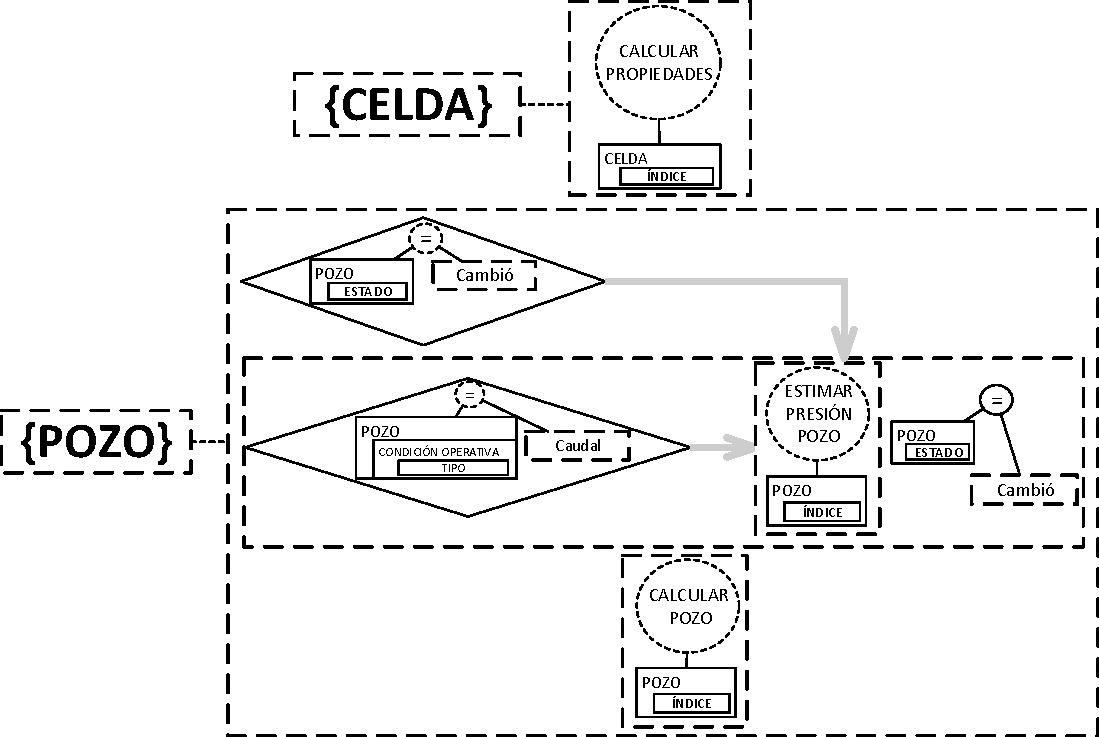
\includegraphics[width=\linewidth]{Fig/TiempoK.pdf}%
	%\caption{Complete PS Representation for EOR Processes} \label{fig:PSComplete}
	\caption[Recálculo de Propiedades al término actual para la iteración.]{Recálculo de Propiedades al término actual para la iteración. Los autores.} \label{fig:TimeK}
\end{figure}

\begin{figure}[h]
	\centering%
	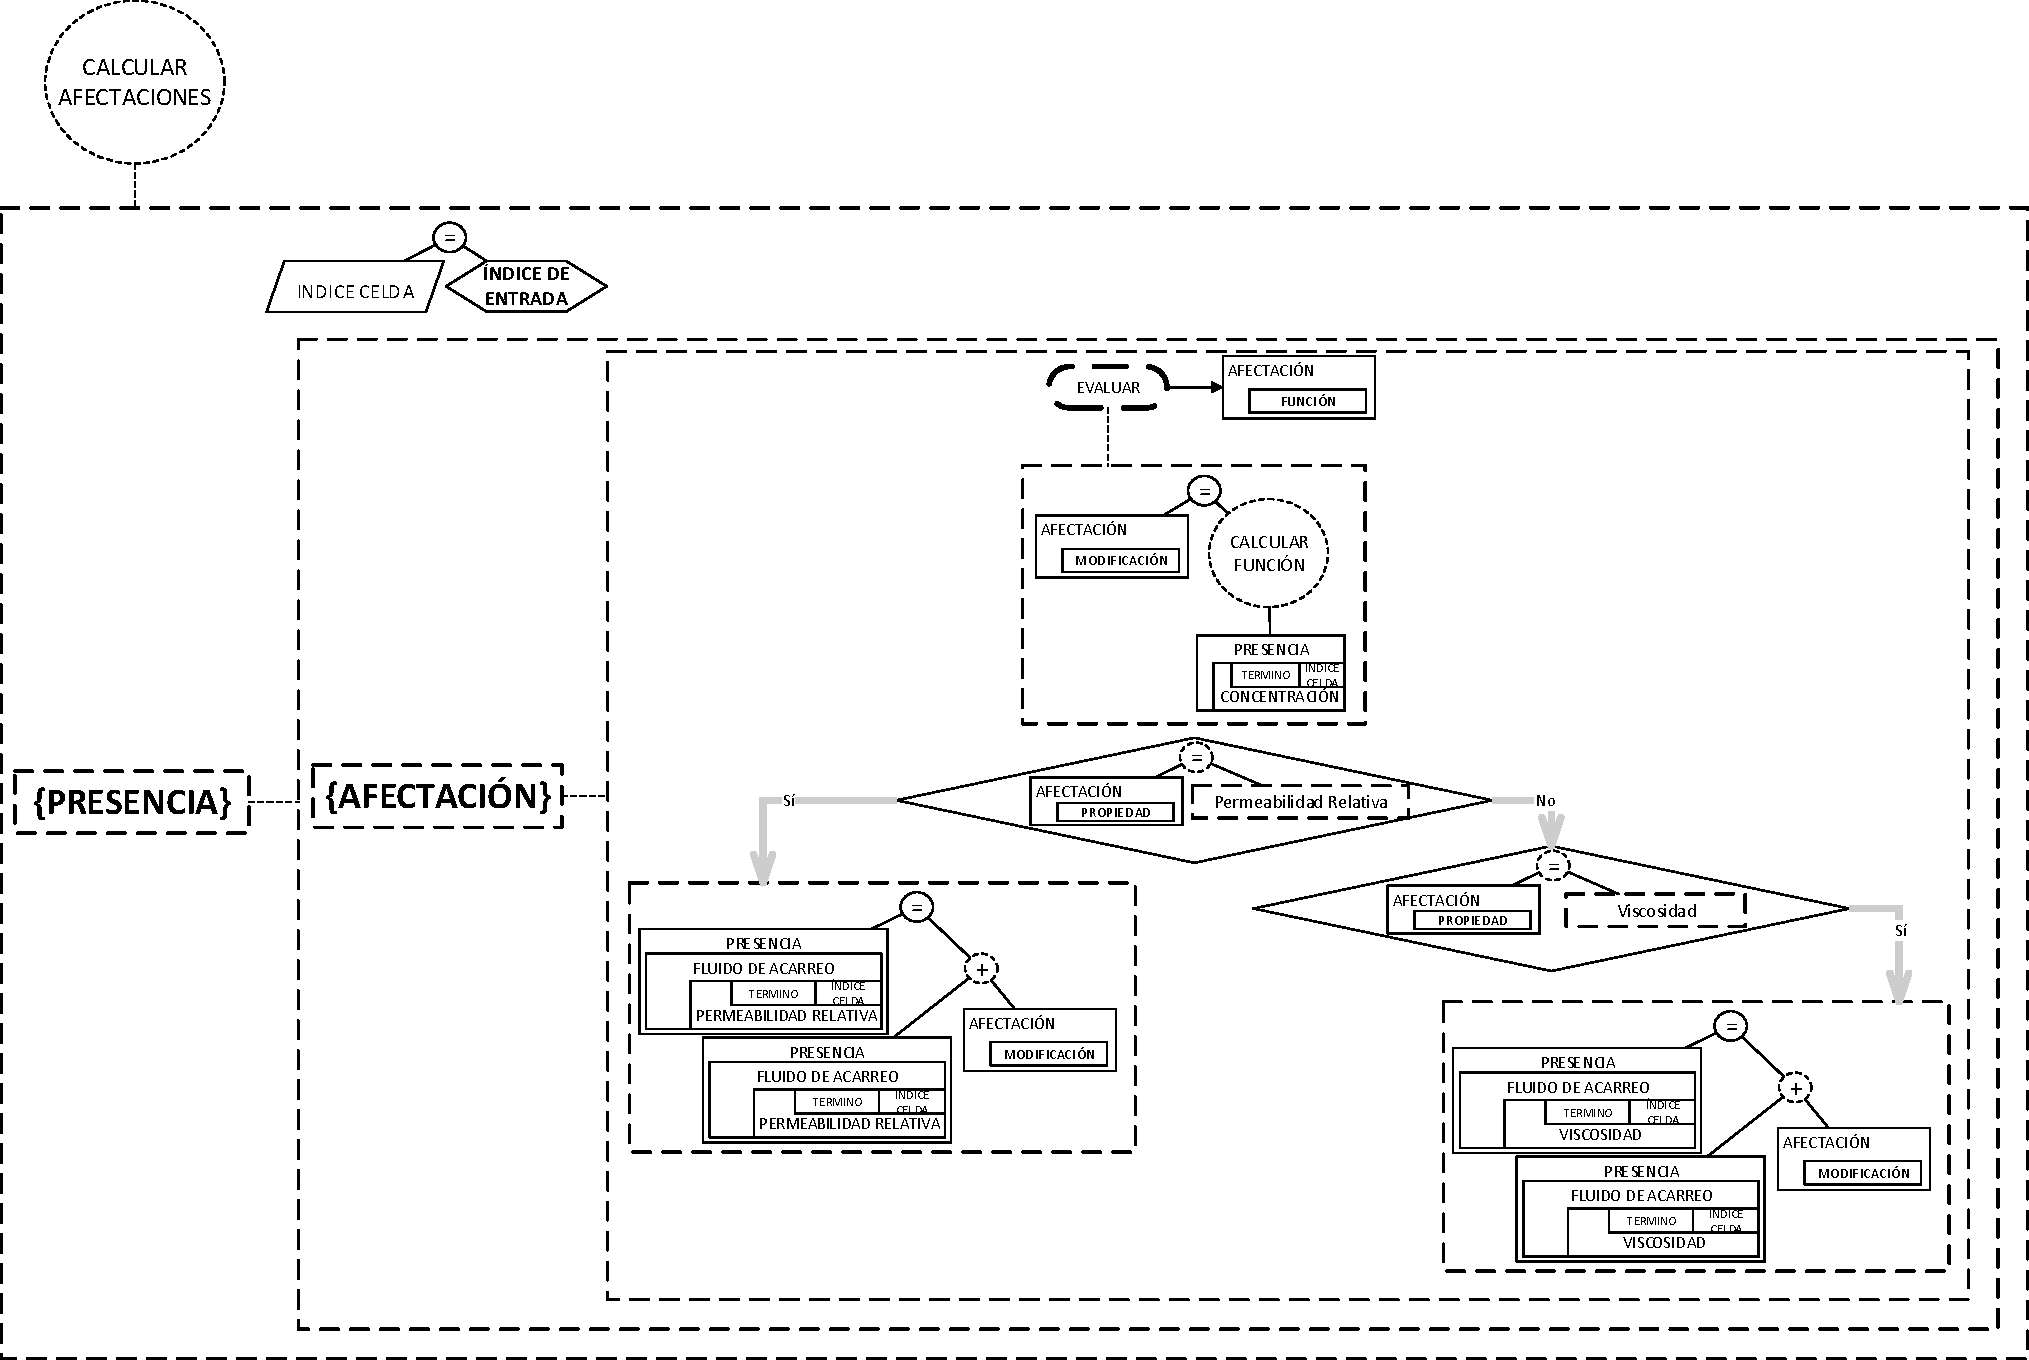
\includegraphics[width=\linewidth]{Fig/CalcularAfectaciones.pdf}%
	%\caption{Complete PS Representation for EOR Processes} \label{fig:PSComplete}
	\caption[Función calcular afectaciones.]{Función calcular afectaciones. Los autores.} \label{fig:CalcularAfectaciones}
\end{figure}

\subsubsection{Cálculo de Residuales}\label{subsec:Residual}
En el cálculo de residuales se reúnen las ecuaciones de conservación de volumen del fluido, las ecuaciones para los químicos en cada una de sus presencias, y las ecuaciones de caudal de peaceman multiperforado para pozos. El armado del vector residual para el método de Newton se calcula de manera iterativa, realizando un ciclo sobre el concepto ecuación y calculando dependiendo de si la ecuación es de tipo fluido, presencia o de tipo pozo, cabe aclarar que sólo las ecuaciones de tipo pozo pueden tener como estado ``Inactivas''. Las ecuaciones de tipo fluido y presencia, se procesan del mismo modo, pero difieren en el cálculo del residual.\\

Las ecuaciones de cada presencia del químico y de los fluidos se evalúan en todas las celdas, mientras que las ecuaciones de cada pozo se evalúan únicamente en las celdas con perforaciones o ``perforados'', por lo tanto se requiere diferenciar su cálculo de residual según el tipo. Para obtener la ubicación del residual en su correspondiente vector, se requiere conocer el tipo de ecuación que se está calculando. Adicionalmente se emula una sobre-escritura u \textit{override} de los residuales de químico y de fluido, generando una función intermedia ``calcular residual'' en la que se define si se ejecuta ``calcular residual fluido'' o ``calcular residual químico''. Esto permite generalizar el cálculo del residual para una ecuación que se evalúe en toda la malla. La función ``calcular residual'' se muestra en la Figura \ref{fig:CalResidual}.\\

Es importante notar también, que la función ``ubicar'' se encarga de calcular la posición correspondiente en el vector residual que agrupa todas las incógnitas a resolver. El proceso de cálculo de residuales se muestra en la Figura \ref{fig:Residual}. El residual de fluidos, de presencias, al igual que de pozos, se muestran en las Figuras \ref{fig:ResidualFluid}, \ref{fig:ResidualChemical} \ref{fig:ResidualWell}. Las funciones de flujo y acumulación, que corresponden a las ecuaciones discretizadas generalizadas del fluido en la Subsección \ref{subsec:PS_Equilibrium}, se muestran en las Figuras \ref{fig:Accumulation} y \ref{fig:Flow}. Las ecuaciones discretizadas del químico se muestran en las Figuras \ref{fig:ChemicalAccumulation}, \ref{fig:ChemicalFlow}, \ref{fig:ChemicalTransferences}.\\ % Residual

\begin{figure}[h]
	\centering%
	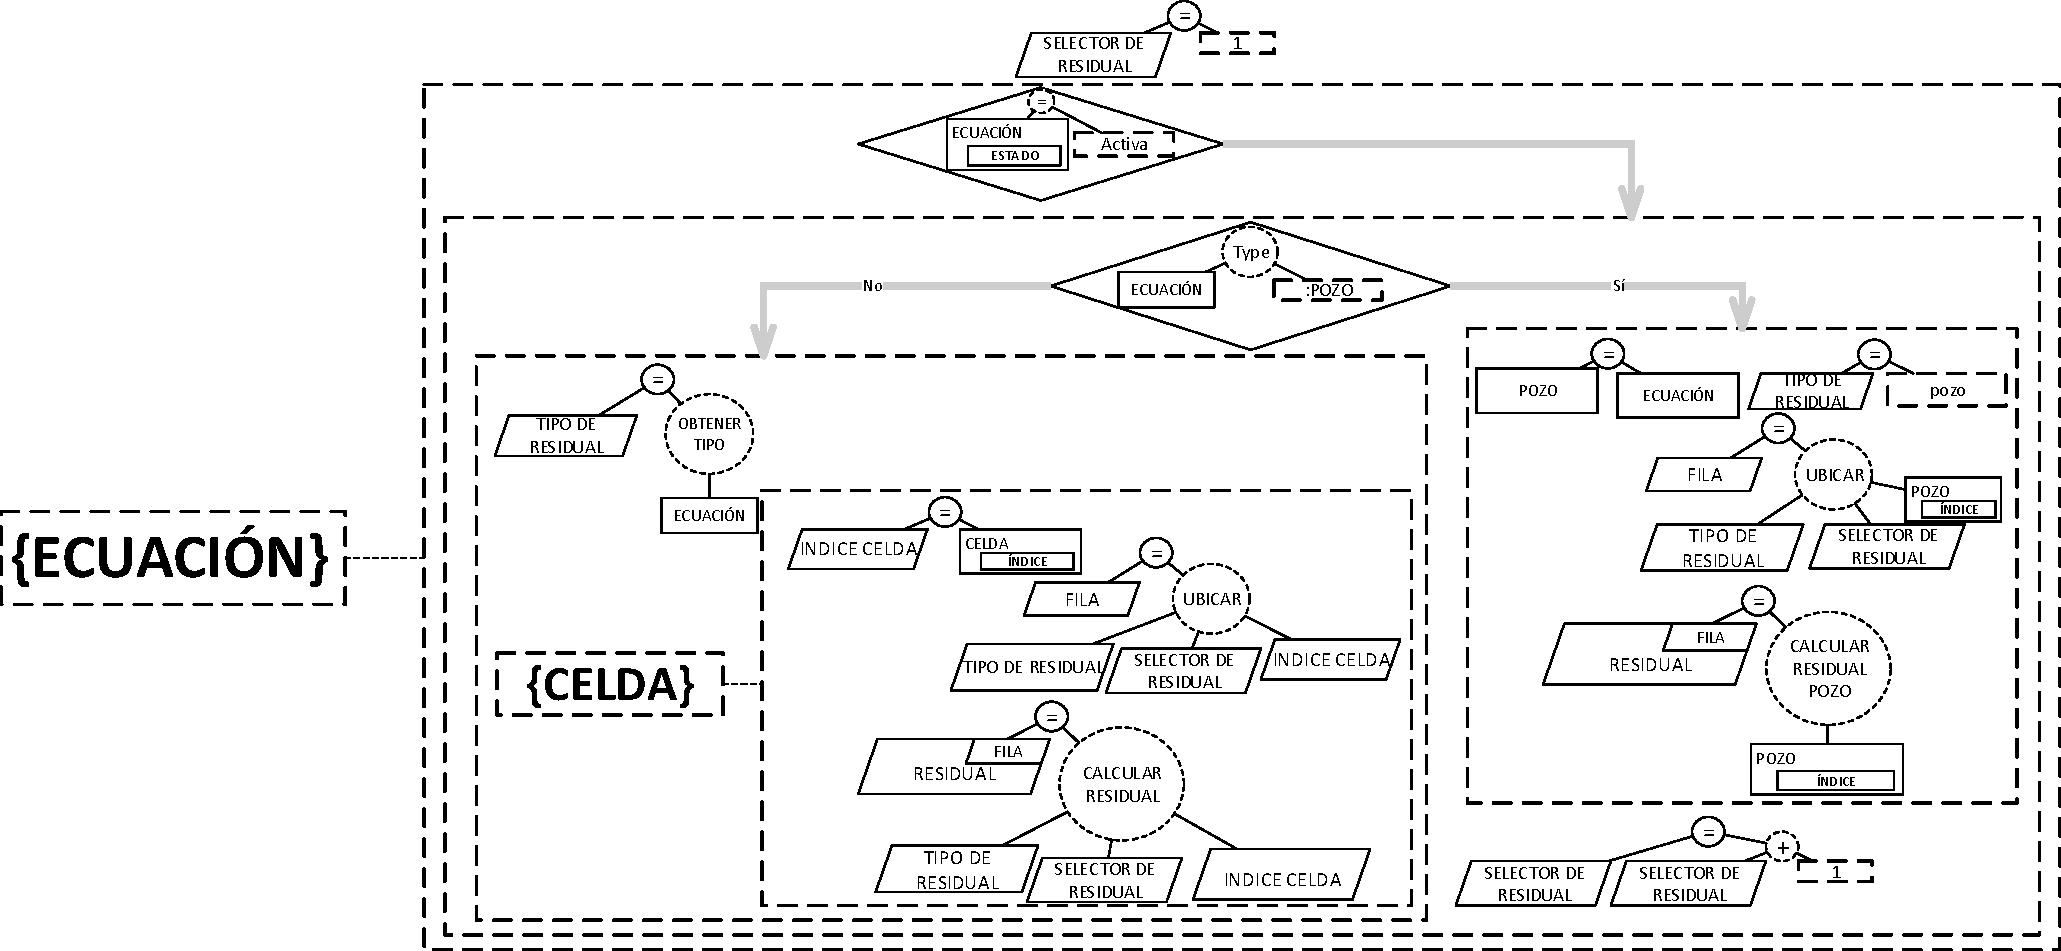
\includegraphics[width=\linewidth]{Fig/Residual.pdf}%
	%\caption{Complete PS Representation for EOR Processes} \label{fig:PSComplete}
	\caption[Cálculo de residual para la iteración.]{Cálculo de residual para la iteración. Los autores.} \label{fig:Residual}
\end{figure}


\begin{figure}[h]
	\centering%
	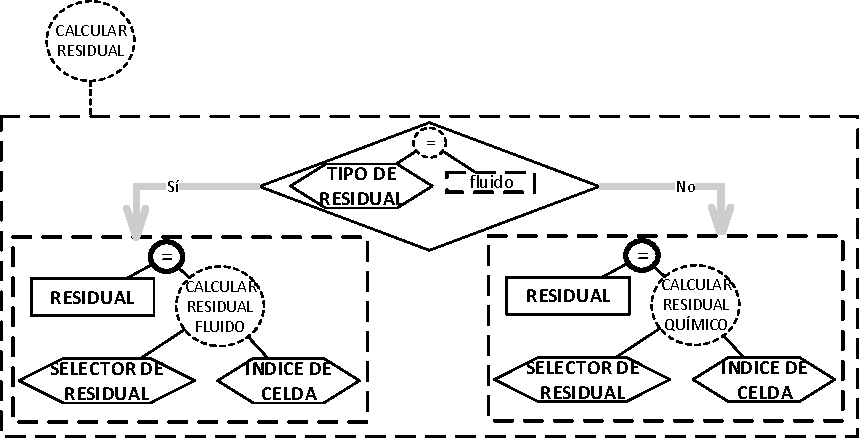
\includegraphics[width=0.7\linewidth]{Fig/CalcularResidual.pdf}%
	%\caption{Complete PS Representation for EOR Processes} \label{fig:PSComplete}
	\caption[Cálculo de residual por tipo.]{Cálculo de residual por tipo. Los autores.} \label{fig:CalResidual}
\end{figure}

\begin{figure}[h]
	\centering%
	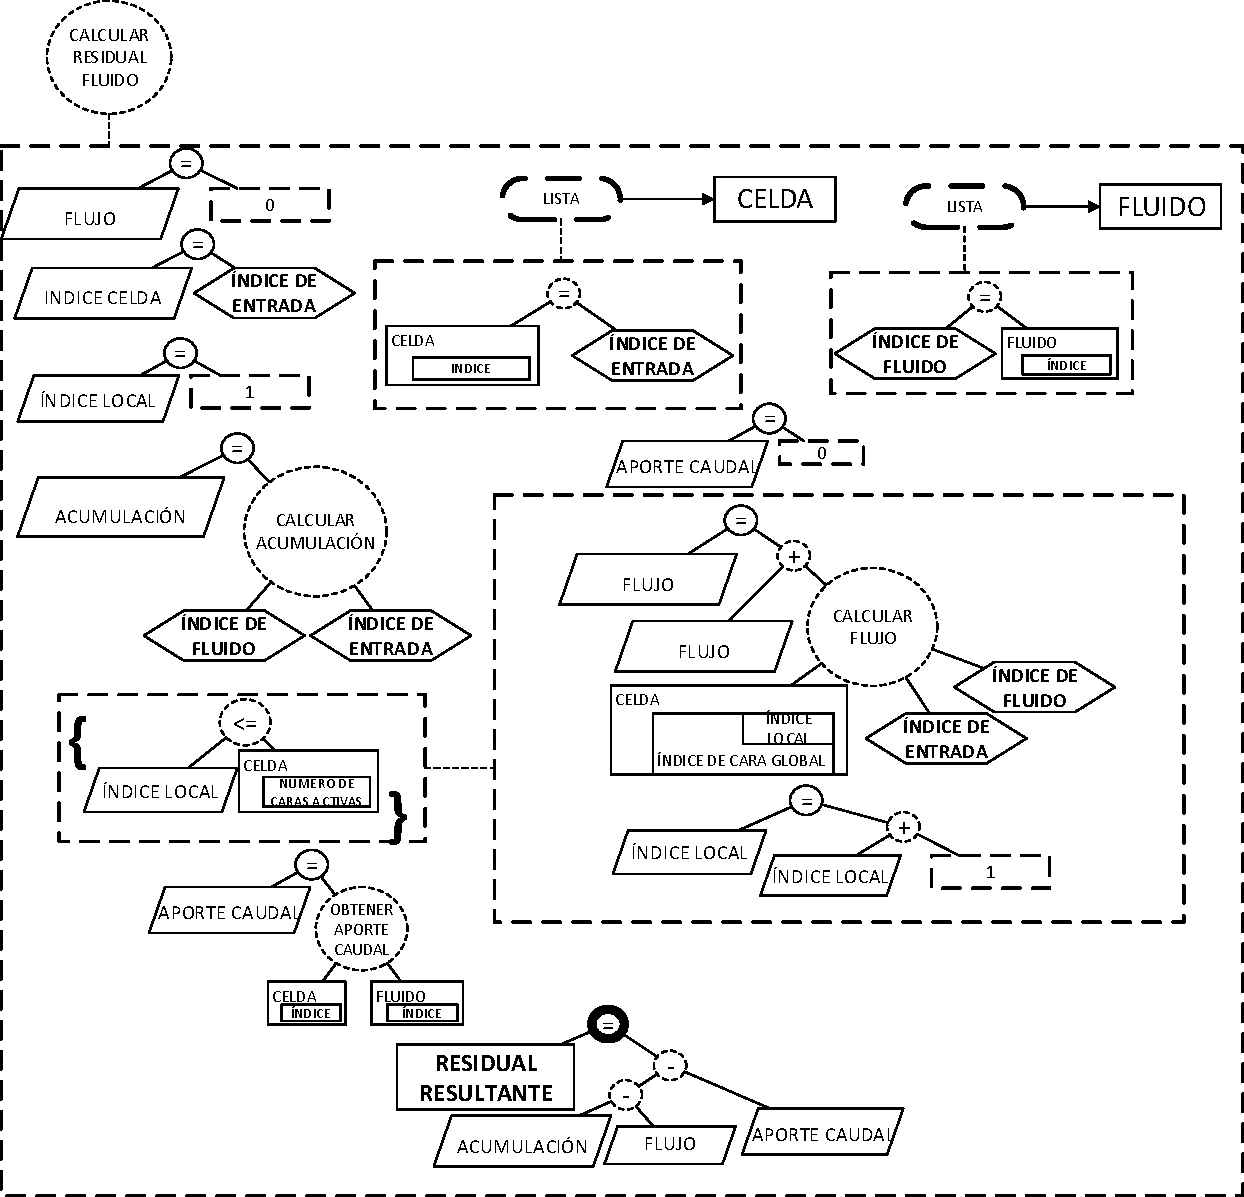
\includegraphics[width=0.9\linewidth]{Fig/CalcularResidualFluido.pdf}%
	%\caption{Complete PS Representation for EOR Processes} \label{fig:PSComplete}
	\caption[Cálculo de residual de un fluido.]{Cálculo de residual de un fluido. Los autores.} \label{fig:ResidualFluid}
\end{figure}

\begin{figure}[h]
	\centering%
	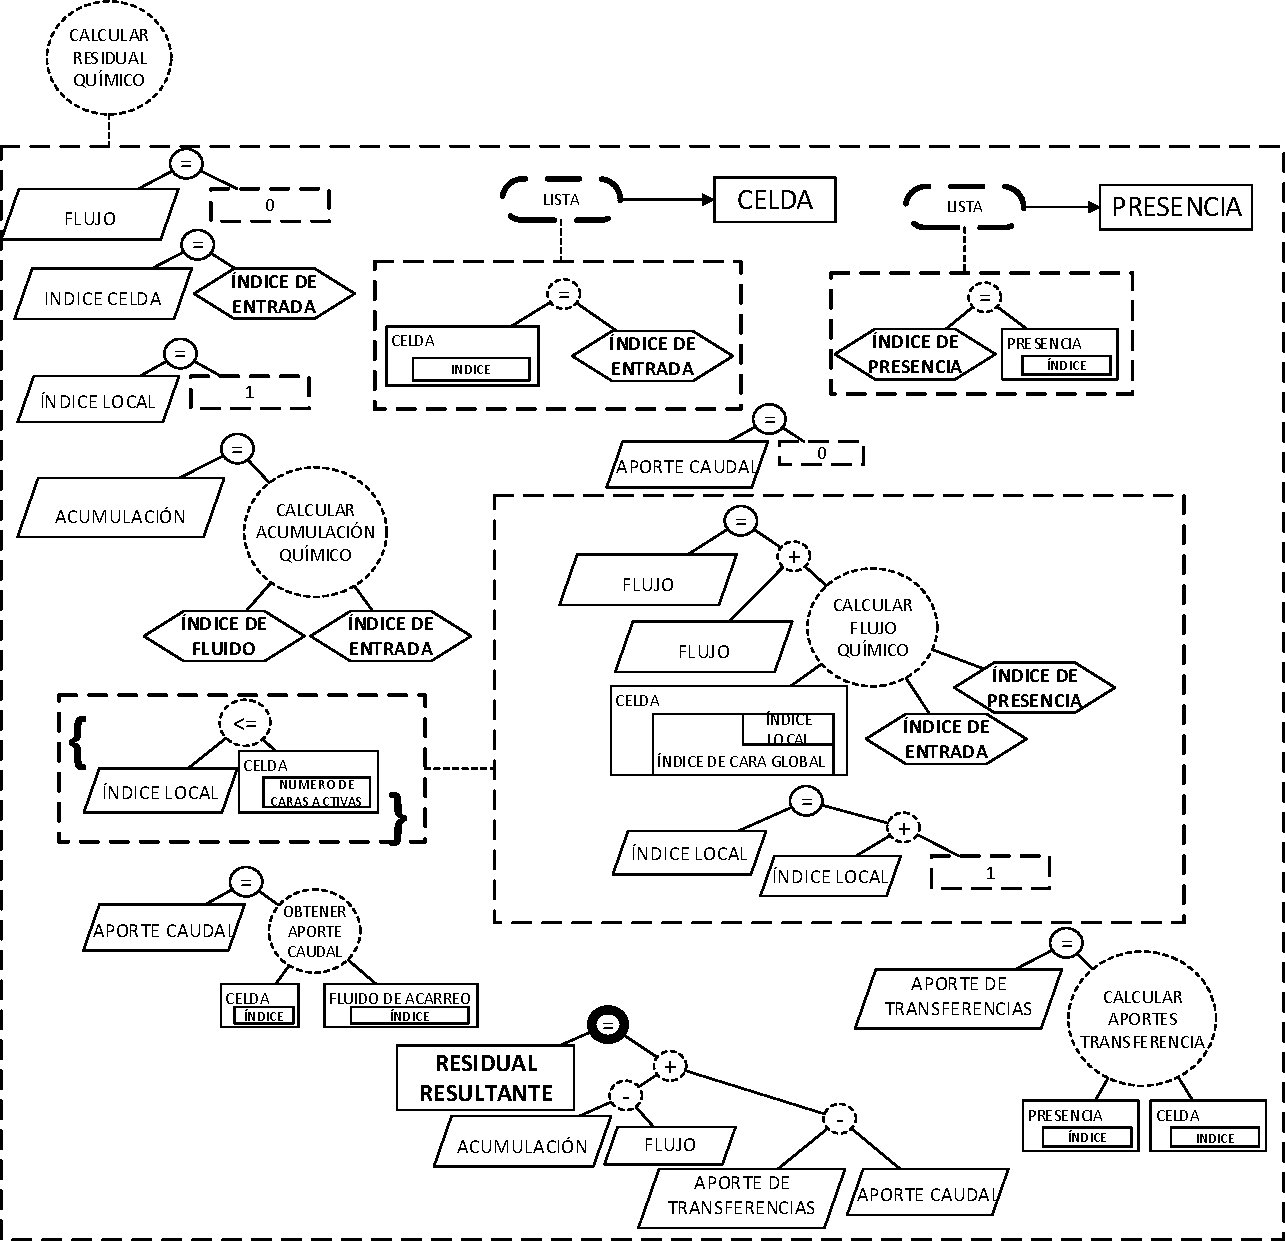
\includegraphics[width=0.9\linewidth]{Fig/CalcularResidualQuimico.pdf}%
	%\caption{Complete PS Representation for EOR Processes} \label{fig:PSComplete}
	\caption[Cálculo de residual de una presencia.]{Cálculo de residual de una presencia (Químico-Fluido). Los autores.} \label{fig:ResidualChemical}
\end{figure}

\begin{figure}[h]
	\centering%
	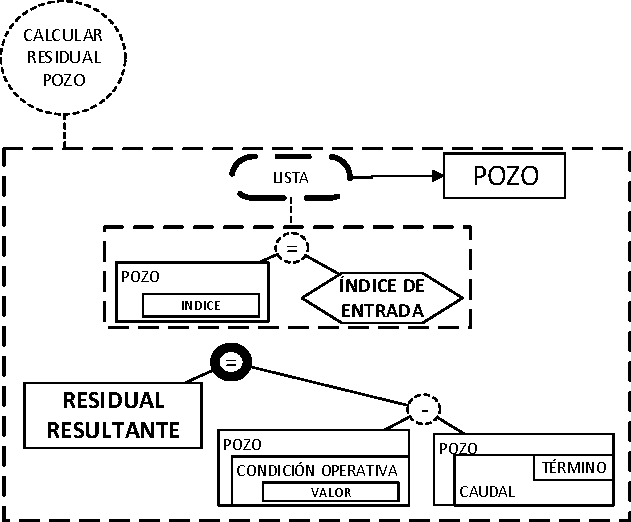
\includegraphics[width=0.7\linewidth]{Fig/CalcularResidualPozo.pdf}%
	%\caption{Complete PS Representation for EOR Processes} \label{fig:PSComplete}
	\caption[Cálculo de residual de pozo.]{Cálculo de residual de pozo. Los autores.} \label{fig:ResidualWell}
\end{figure}
\begin{figure}[h]
	\centering%
	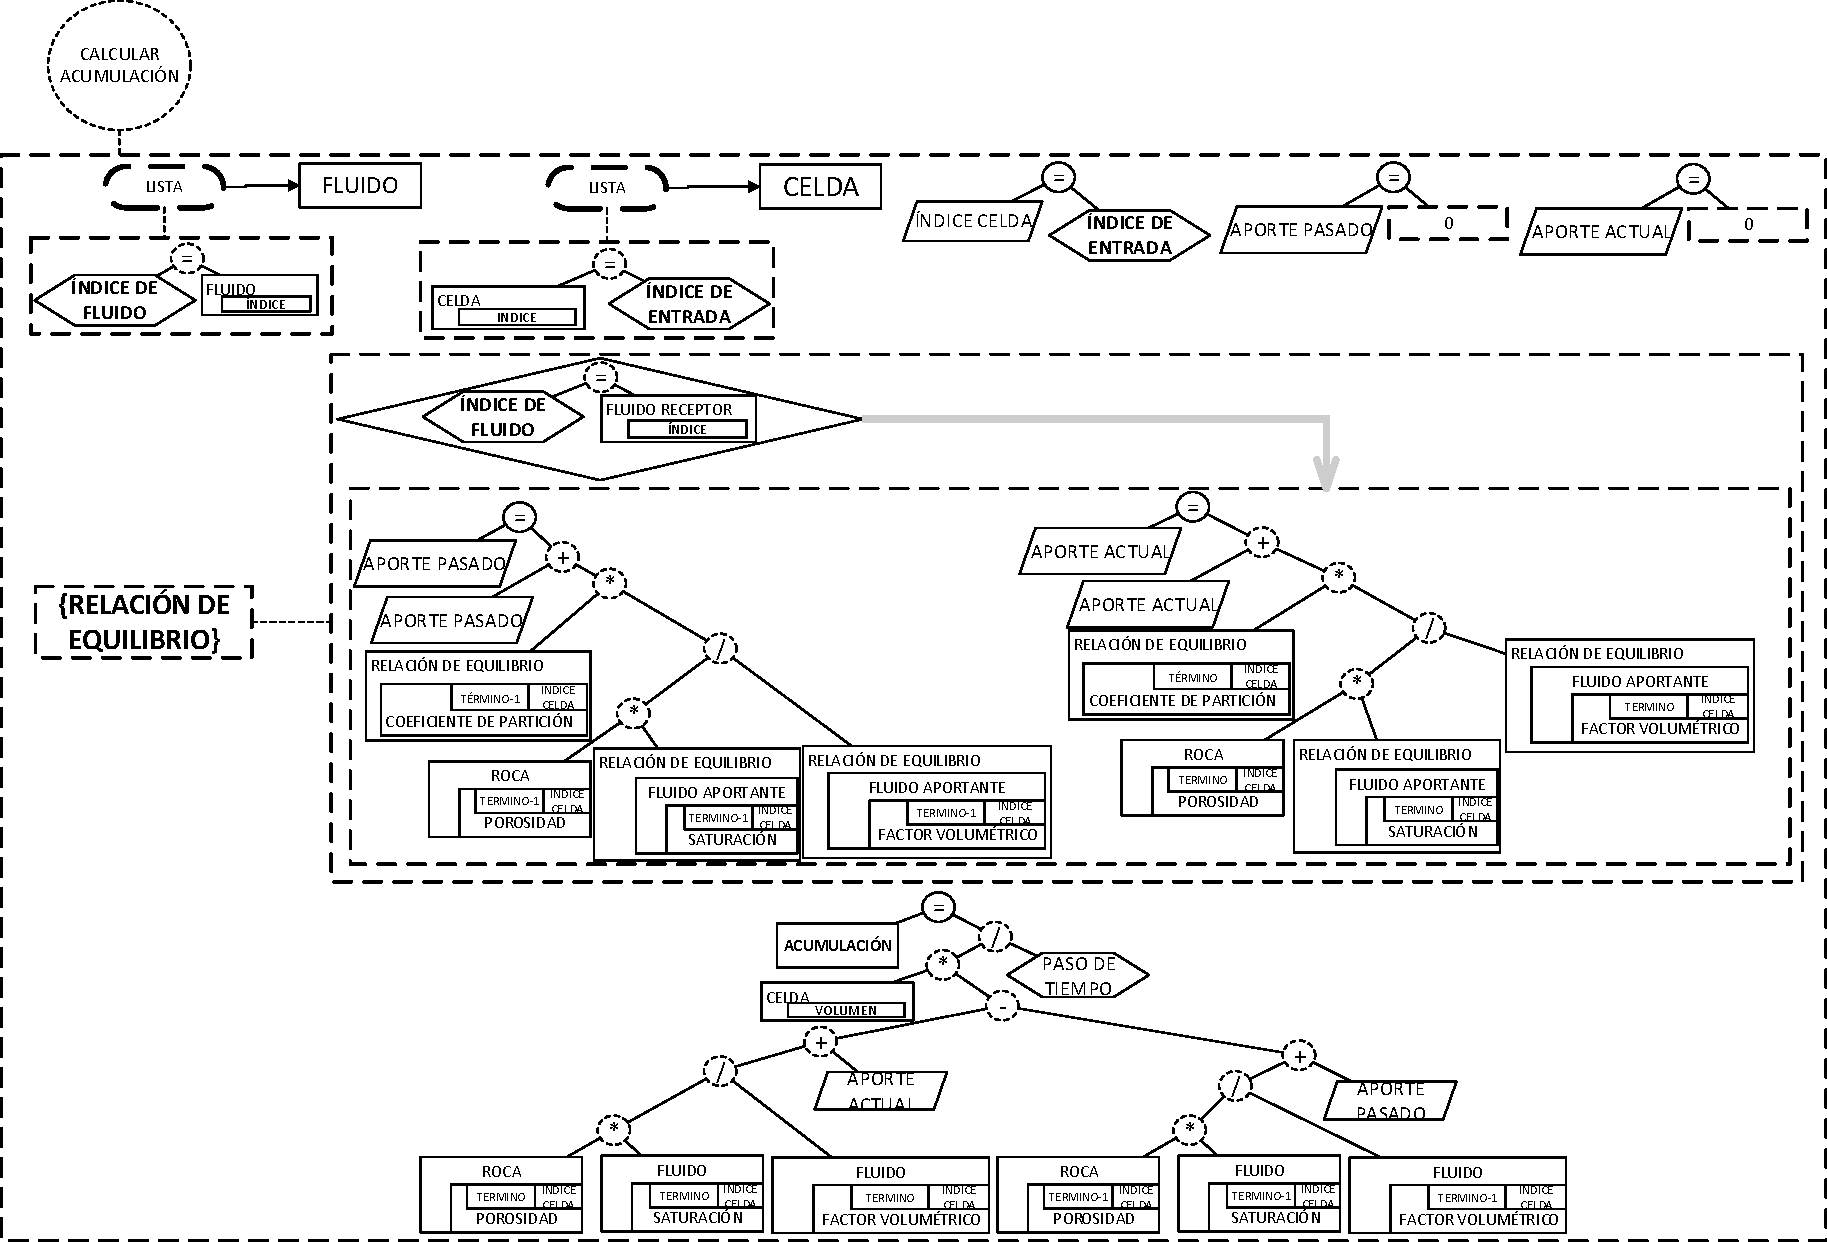
\includegraphics[width=0.9\linewidth]{Fig/CalcularAcumulacion.pdf}%
	%\caption{Complete PS Representation for EOR Processes} \label{fig:PSComplete}
	\caption[Cálculo de acumulación generalizado.]{Cálculo de acumulación generalizado. Los autores.} \label{fig:Accumulation}
\end{figure}
\begin{figure}[h]
	\centering%
	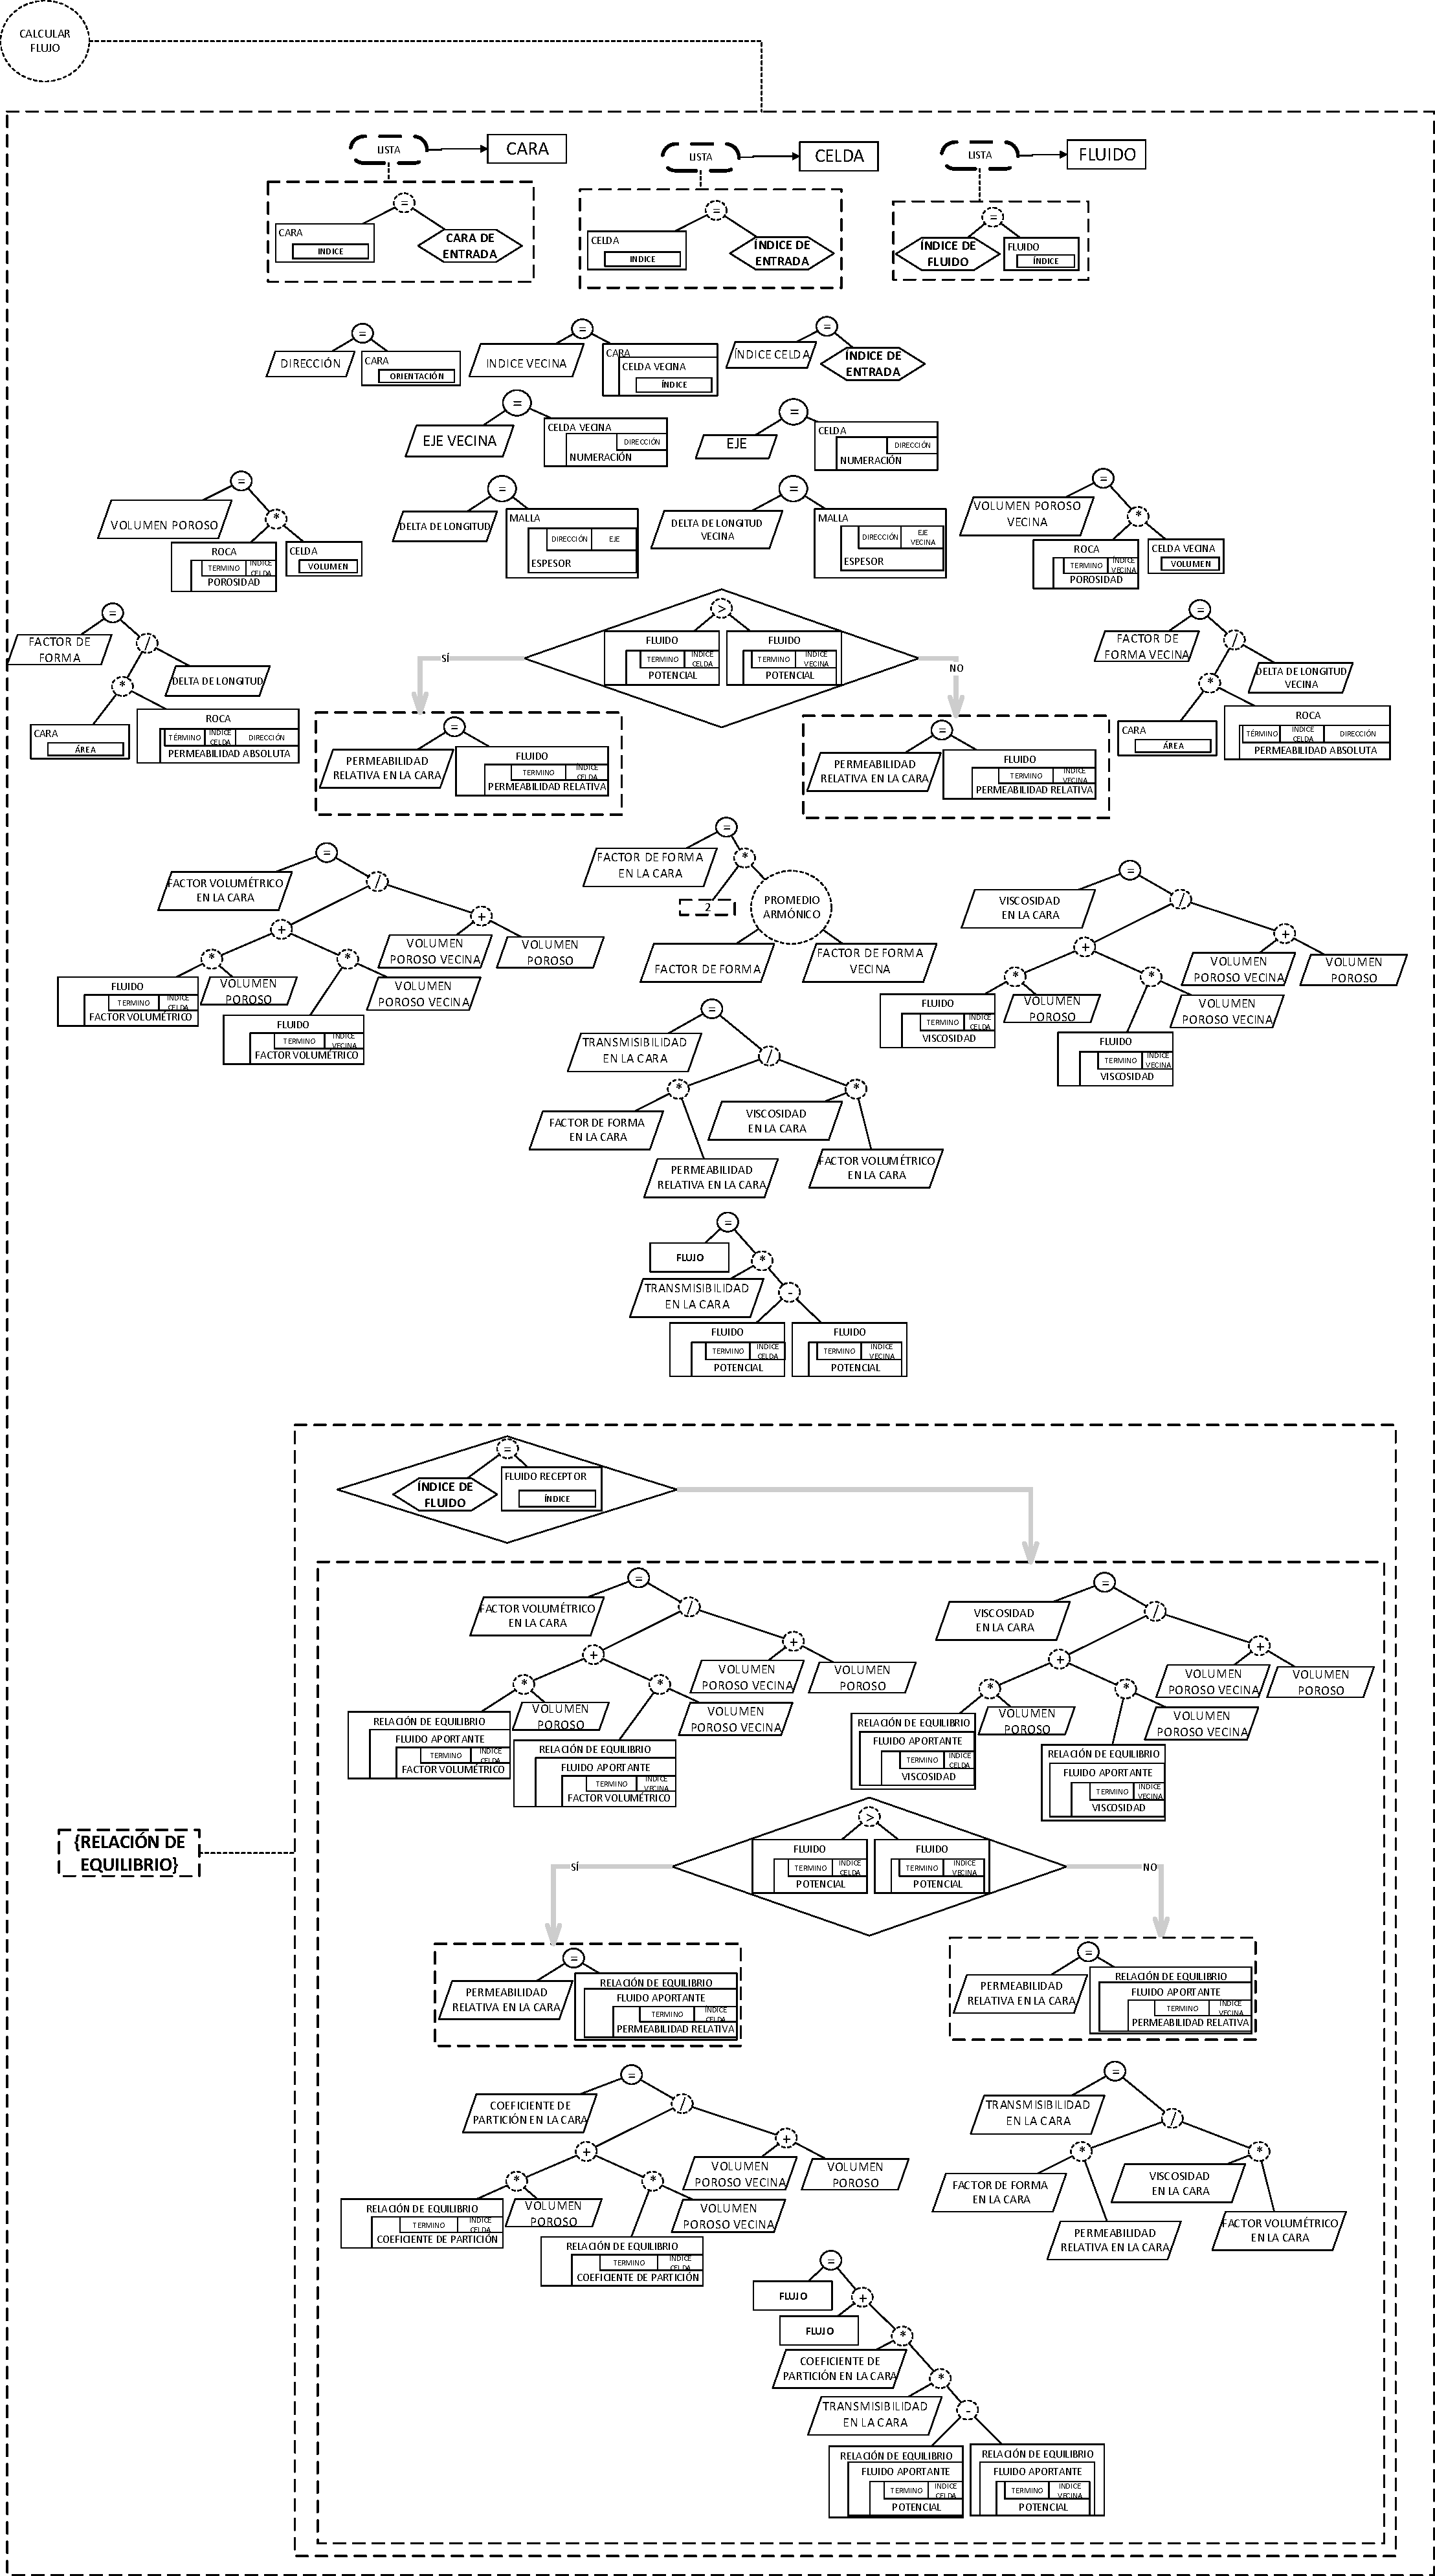
\includegraphics[height=0.9\textheight]{Fig/CalcularFlujo.pdf}%
	%\caption{Complete PS Representation for EOR Processes} \label{fig:PSComplete}
	\caption[Cálculo de flujo generalizado.]{Cálculo de flujo generalizado. Los autores.} \label{fig:Flow}
\end{figure}

\begin{figure}[h]
	\centering%
	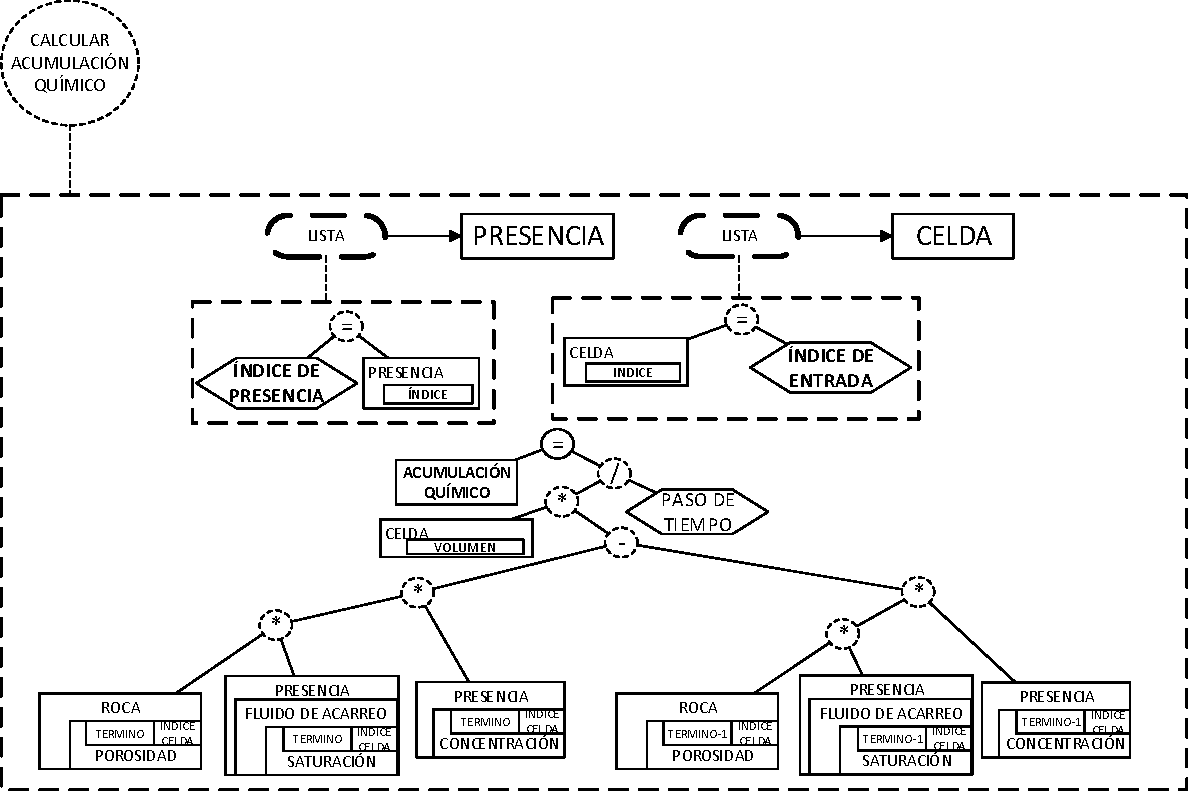
\includegraphics[width=0.7\linewidth]{Fig/CalcularAcumulacionQuimico.pdf}%
	%\caption{Complete PS Representation for EOR Processes} \label{fig:PSComplete}
	\caption[Cálculo de acumulación para el químico.]{Cálculo de acumulación para el químico. Los autores.} \label{fig:ChemicalAccumulation}
\end{figure}

\begin{figure}[h]
	\centering%
	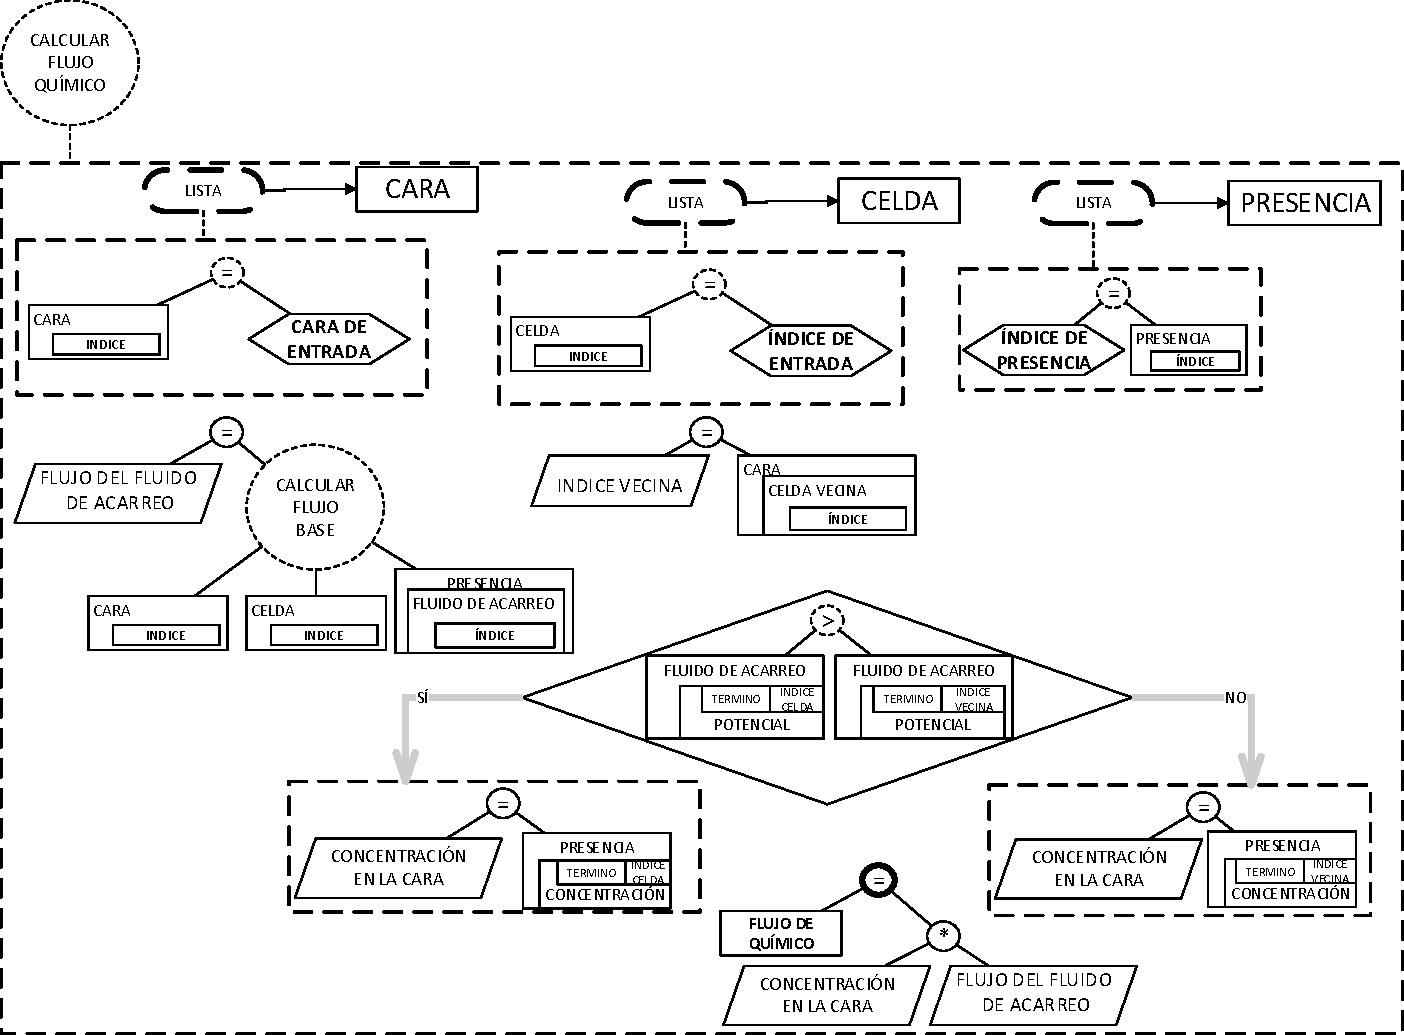
\includegraphics[width=0.9\linewidth]{Fig/CalcularFlujoQuimico.pdf}%
	%\caption{Complete PS Representation for EOR Processes} \label{fig:PSComplete}
	\caption[Cálculo de flujo para el químico.]{Cálculo de flujo para el químico. Los autores.} \label{fig:ChemicalFlow}
\end{figure}

\begin{figure}[h]
	\centering%
	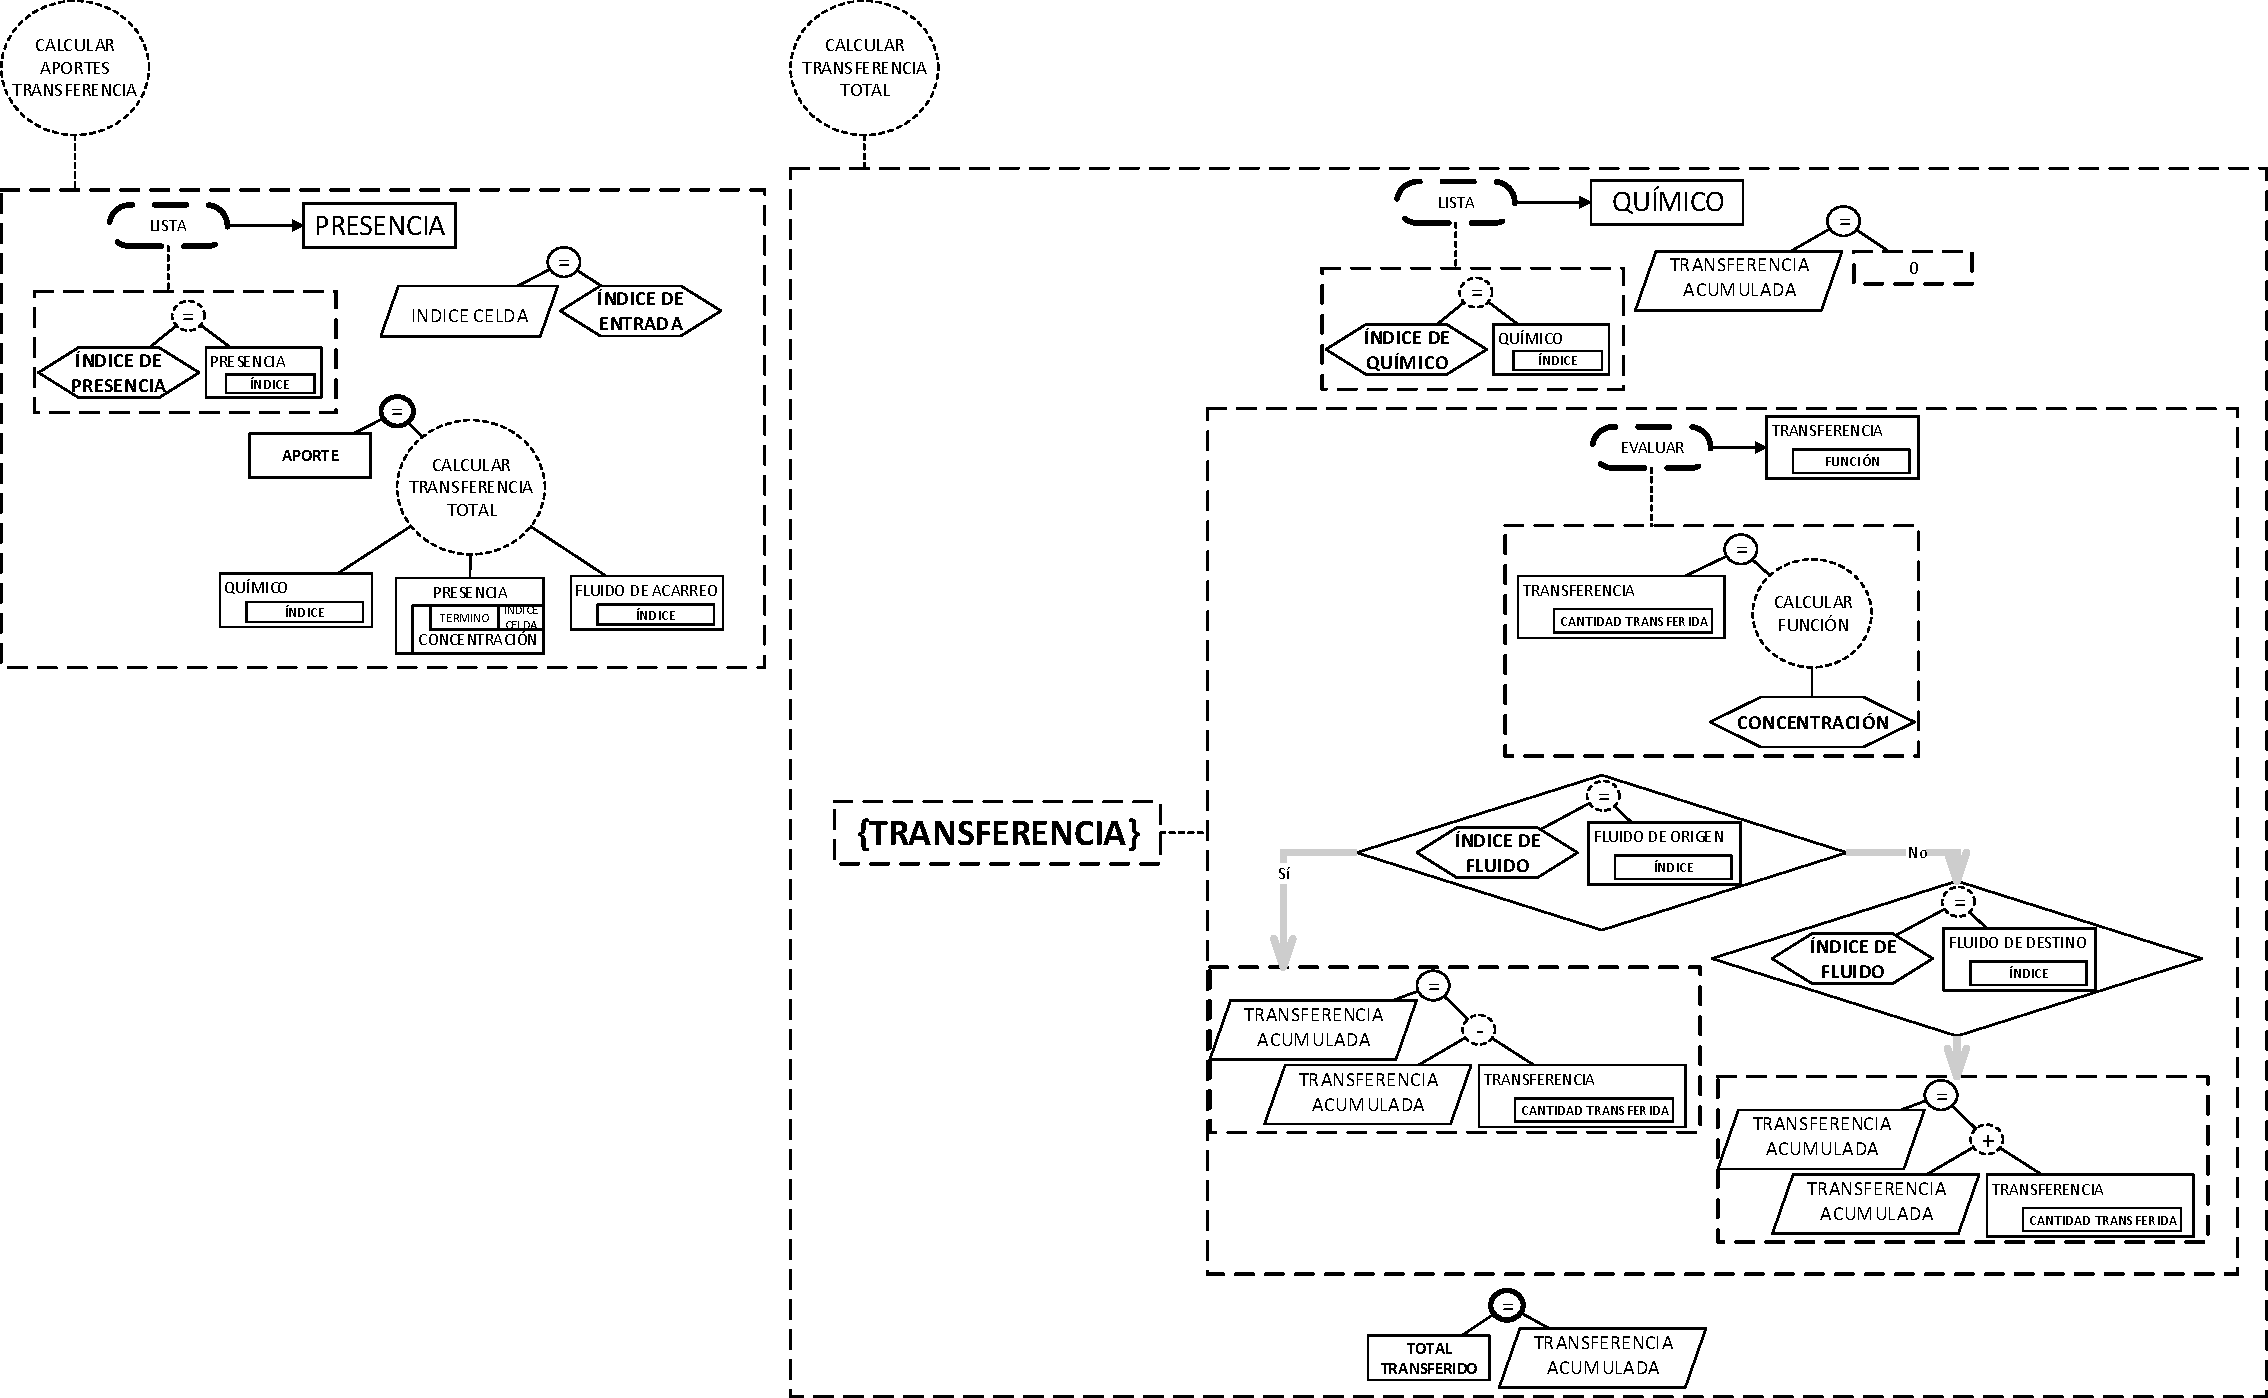
\includegraphics[width=0.9\linewidth]{Fig/CalcularTransferencias.pdf}%
	%\caption{Complete PS Representation for EOR Processes} \label{fig:PSComplete}
	\caption[Cálculo de la masa total transferida desde la presencia.]{Cálculo de la masa total transferida desde la presencia. Los autores.} \label{fig:ChemicalTransferences}
\end{figure}

Se puede notar que, a pesar de que, la representación del flujo del fluido y del químico tiene elementos en común, es necesario representarlos aparte, puesto que la ecuación discretizada del flujo del químico en los distintos fluidos no considera relaciones de equilibrio. Adicionalmente, en las ecuaciones del químico se considera transferencias de masa entre diferentes fluidos.

\subsubsection{Cálculo de la función Jacobiana}
El armado de la matriz jacobiana consiste de dos ciclos anidados, donde el primer ciclo corresponde al recorrido por residuales, y el segundo a la variable respecto a la cuál se deriva. Se recorren las ecuaciones para modificar la variable principal de cada ecuación, sea fluido, presencia o de pozo, y calcular el correspondiente residual. Este cálculo está presente en la Figura \ref{fig:FluidPressureVaries}.

\subsubsection{Solución del sistema lineal y actualización de incógnitas}
Por último una vez se tiene la matriz del jacobiano construida se soluciona usando el operador ``Bigradiente conjugado estabilizado", proveniente de alguna librería, que resuelve el sistema: $Jacobiano*DeltaDeSolucion = -Residual$ como se observa en la Figura \ref{fig:LinearSystem}. Posteriormente, se actualizan las incógnitas sumándoles el delta de solución de manera acorde al cálculo del residual. Esto se presenta en la Figura \ref{fig:UpdateVariables}.

\begin{figure}[h]
	\centering%
	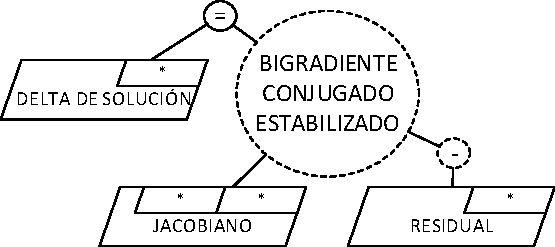
\includegraphics[scale=1]{Fig/SistemaLineal.pdf}%
	%\caption{Complete PS Representation for EOR Processes} \label{fig:PSComplete}
	\caption[Sistema lineal resultante del método de Newton-Raphson.]{Sistema lineal resultante del método de Newton-Raphson. Los autores.} \label{fig:LinearSystem}
\end{figure}

\begin{figure}[h]
	\centering%
	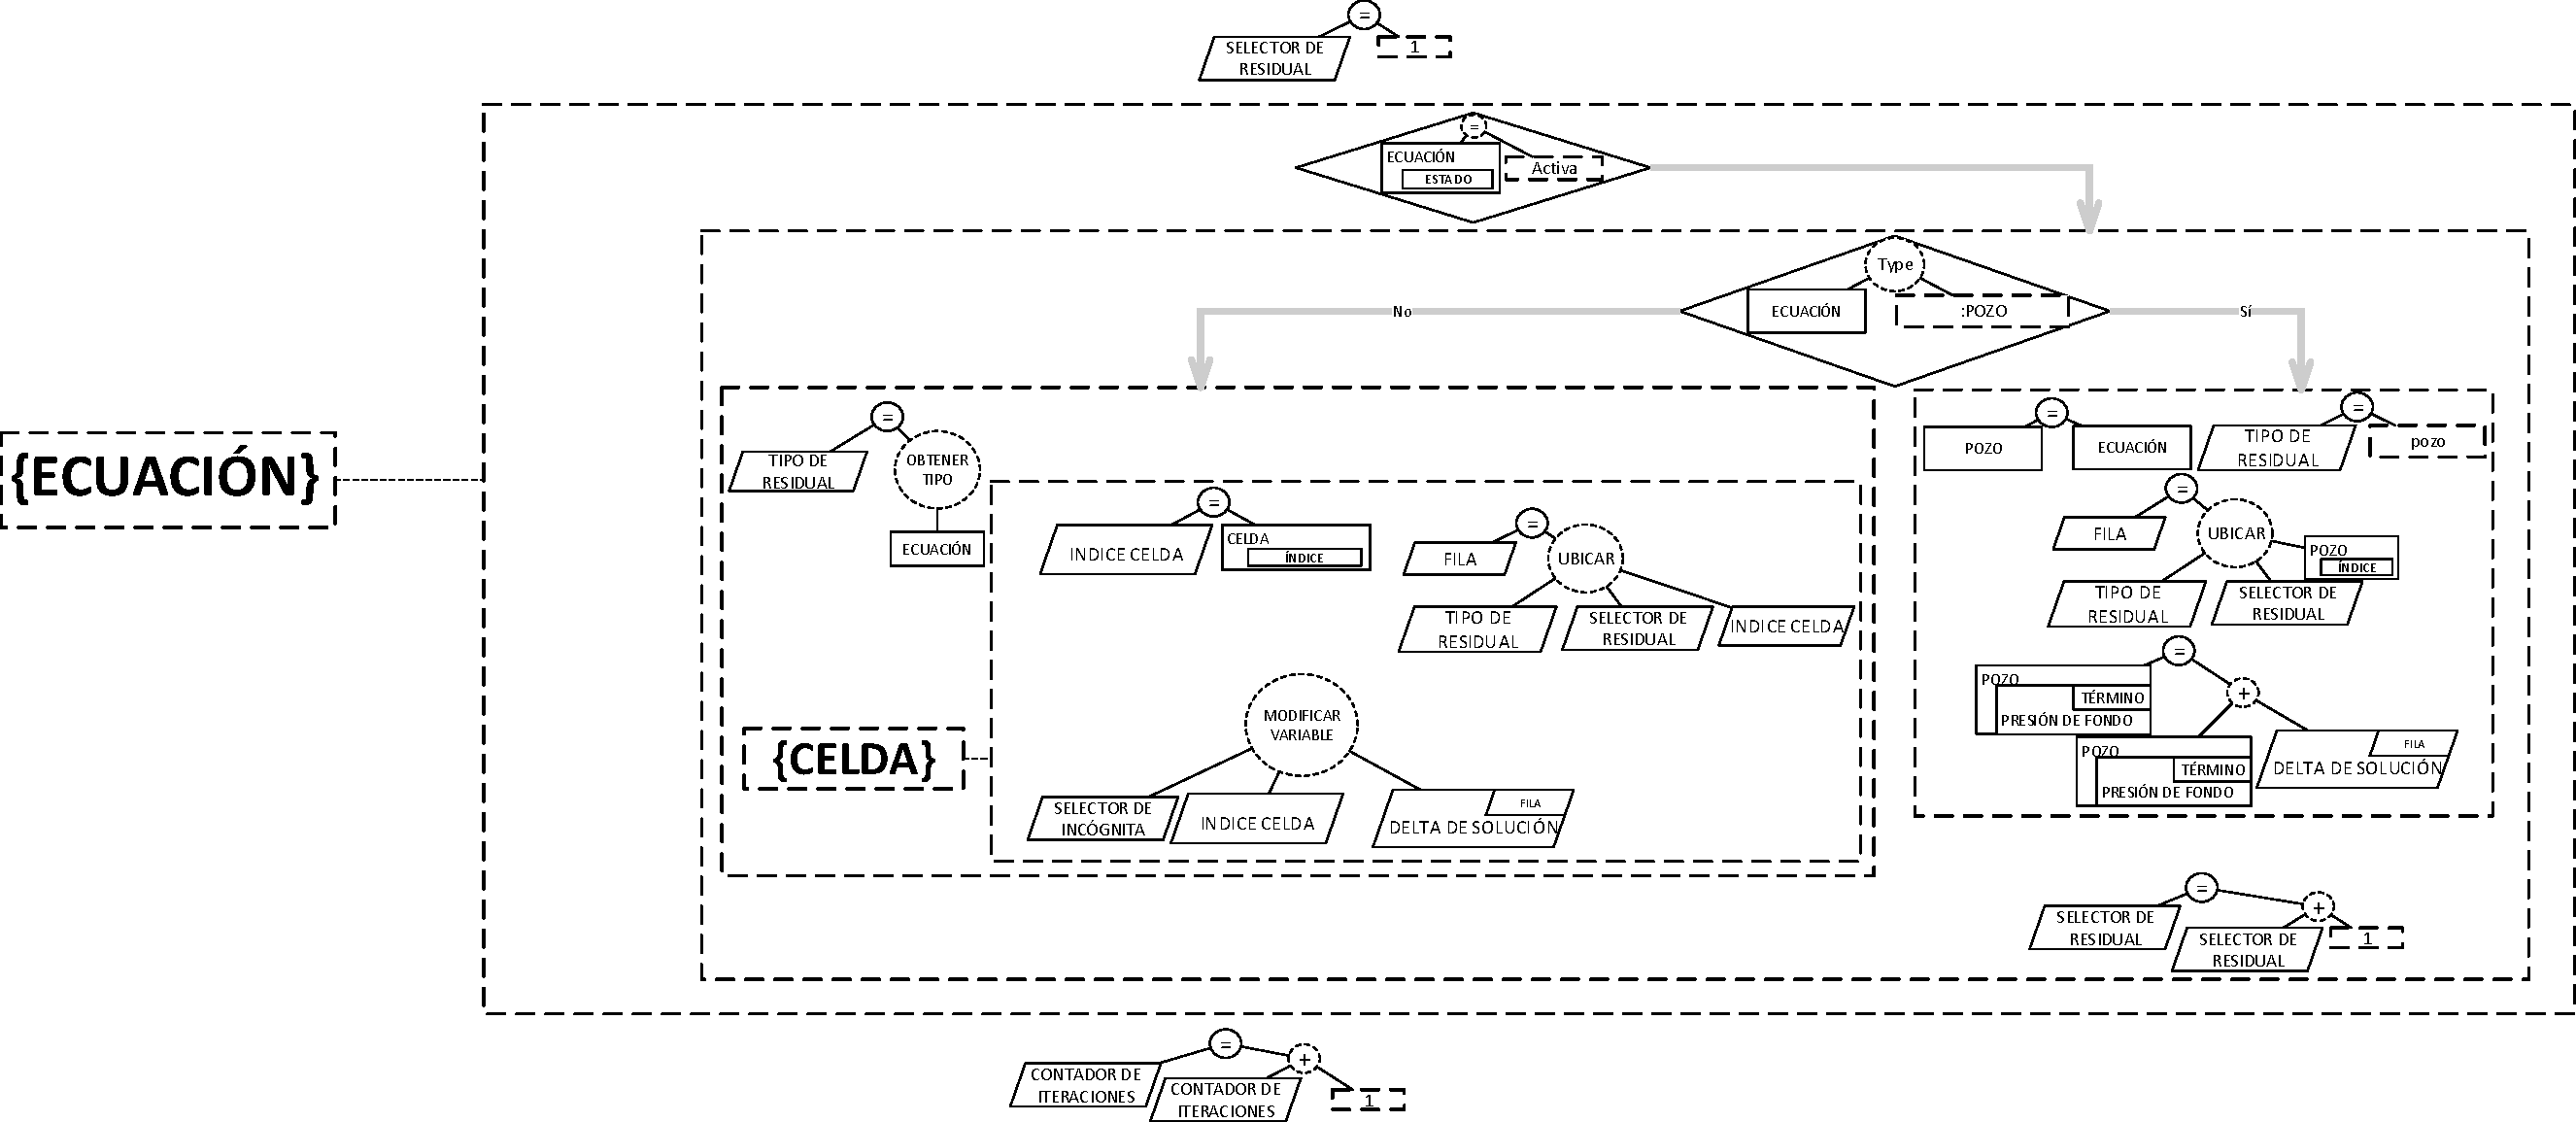
\includegraphics[width=\linewidth]{Fig/ActualizacionDeIncognitas.pdf}%
	%\caption{Complete PS Representation for EOR Processes} \label{fig:PSComplete}
	\caption[Recálculo de Propiedades al término actual para la iteración.]{Recálculo de Propiedades al término actual para la iteración. Los autores.} \label{fig:UpdateVariables}
\end{figure}
%includefigure{Graphical Representation of subroutine}

%includegraphic{Code Translation}

%Se deben incluir tantos cap\'{\i}tulos como se requieran; sin embargo, se recomienda que la tesis  o trabajo de investigaci\'{o}n tenga un m\'{\i}nimo 3 cap\'{\i}tulos y m\'{a}ximo de 6 cap\'{\i}tulos (incluyendo las conclusiones).\\